%%%%%%%%%%%%%%%%%%%%%%%%%%%%%%%%%%%%%%%%%%%%%%%%%%%%%%%%%
% Niniejszy plik przedstawia przykładowy skład pracy dyplomowej na Wydziale Matematyki PWr. 
% 
% Autorzy: Damian Fafuła, Michał Kijaczko, Jakub Michalczak, Maciej Miśta Dagmara Nowak, Tomasz Skalski, Wojciech Słomian
% Data utworzenia: 8.05.2018
%
% Zmodyfikowane przez: Jakuba Ślęzaka 
% Data utworzenia aktualnej wersji: 28.01.2025 
% Numer wersji: 1.1
%
% Poniższą formatkę można rozpowszechniać i edytować pod warunkiem zachowania numeru wersji, 
% informacji o autorach i dodaniu informacji o wprowadzonych zmianach.
%
%                          OPCJE
%%%%%%%%%%%%%%%%%%%%%%%%%%%%%%%%%%%%%%%%%%%%%%%%%%%%%%%%%

% Następna linia zaczyna kolejne rozdziały od stron nieparzystych
\def\rodzialyOdNieparzystych {wybrane}
% zakomentować ją, jeżeli rozdziały są krótkie i nie jest to wskazane.

% Następna linia zaznacza kolorami interaktywne linki w pliku pdf
\def\koloroweLinki {wybrane}
% zakomentować ją, aby były czarno białe, np. do druku

% Opcje strony tytułowej:
% Domyślną opcją jest: praca magisterska, język polski.
% W przypadku pracy pisanej w języku angielskim dodajemy opcję [english].
% Dla pracy licencjackiej dodajemy opcję [licencjacka].
% Dla pracy inżynierskiej dodajemy opcję [inzynierska].
% Dopuszczalne są podwójne opcje, np. [licencjacka, english].
% Opcje dodajemy w kwadratowym nawiasie przy \documentclass.
%
%
%%%%%%%%%%%%%%%%%%%%%%%%%%%%%%%%%%%%%%%%%%%%%%%%%%%%%%%%%


\documentclass[english]{pwr_wmat_praca_dyplomowa}
\usepackage{bbm}

\usepackage{color}
\usepackage{todonotes}
\usepackage{marginnote}
\newcommand{\lefttodo}[2][]{{%
 \let\marginpar\marginnote
 \reversemarginpar
 \renewcommand{\baselinestretch}{0.8}%
 \todo[#1]{#2}}}
\usepackage{framed}
\colorlet{shadecolor}{gray!20}


\definecolor{ts}{RGB}{0,0,255}
\newcommand{\ts}[1]{\textcolor{ts}{\bf #1}}
\newcommand{\tsm}[1]{\marginpar{\scriptsize \textcolor{ts}{#1}}}
\newcommand{\tsmm}[1]{\todo[color=ts!20]{#1}}
\newcommand{\mmts}[1]{\lefttodo[color=ts!20]{#1}}

%                       DANE DO PRACY
%%%%%%%%%%%%%%%%%%%%%%%%%%%%%%%%%%%%%%%%%%%%%%%%%%%%%%%%%

% W przypadku pracy dyplomowej w języku angielskim nie jest konieczne 
% wypełnianie pól: \tytul{}, \kierunek{}, \specjalnosc{}, \streszczenie{}, \slowakluczowe{}.
%
% Imię i nazwisko autora
\autor{Jakub Kempa}
%
% Tytuł pracy dyplomowej 
\tytulang{Selected statistical methods in fMRI image denoising}
%
% Tytuł / stopień / imię i nazwisko opiekuna
\opiekun{dr Tomasz Skalski}

% Kierunek studiów po angielsku
\kierunekstudiowang{Applied Mathematics}

% Specjalność w języku angielskim
\specjalnoscang{Modelling, Simulation and Optimization} 

% Krótkie streszczenia po polsku i angielsku, nie dłuższe niż 530 znaków.
\streszczenieang{The thesis focuses on the comparison of selected statistical methods in functional magnetic resonance imaging (fMRI) images denoising. The work focuses on proper data acquisition, correct implementation of methods and accurate comparison of results using metrics commonly used in the field of fMRI. The goal is to find strengths and weaknesses of each method.}
%
% Podajemy najważniejsze słowa kluczowe po polsku i angielsku, w obu przypadkach, max 150 znaków.
\slowakluczoweang{fMRI, denoising, statistical modeling, general linear model, principal component analysis, independent component analysis, cross-validation}
%
%
%%%%%%%%%%%%%%%%%%%%%%%%%%%%%%%%%%%%%%%%%%%%%%%%%%%%%%%%%

% Definicje komend tworzących twierdzenia, definicje, itd, można zmienić wedle uznania.
\newtheorem{theorem}{Theorem}[section]
\newtheorem{proposition}[theorem]{Proposition}
\newtheorem{lemma}[theorem]{Lemma}

\theoremstyle{definition}
\newtheorem{definition}[theorem]{Definition}

\theoremstyle{remark}
\newtheorem{remark}[theorem]{Remark}


%%%%%%%%%%%%%%%%%%%%%%%%%%%%%%%%%%%%%%%%%%%%%%%%%%%%%%%%%%%%%%%%%
\begin{document}
\frontmatter
\maketitle
\mainmatter
\tableofcontents
%\listoffigures
%\listoftables


%%%%%%%%%%%%%%%%%%%%%%%%%%%%%%%%%%%%%%%%%%%%%%%%%%%%%%%%%%%%%%%%%
\chapter{Introduction}

\section{Motivation}

Modern science combines a wide range of engineering and scientific methods to study processes occurring in the human brain. The development of Magnetic Resonance Imaging (MRI), together with methods for measuring changes related to brain activity, led to Functional Magnetic Resonance Imaging (fMRI).

MRI uses the magnetic properties of hydrogen nuclei, which are present in water and other molecules in the human body. A strong static magnetic field partially aligns the nuclear spins. Radio-frequency pulses then disturb this alignment, and after the pulse is switched off, the nuclei slowly return to their rest state. During this process, they generate signals that can be detected by receiver coils. Magnetic field gradients and image reconstruction algorithms are then used to determine the spatial origin of these signals and form an image of the body \cite{fmri}.

However, both biological components and imaging are humanly imperfect. As a result, fMRI data contain several types of noise sources. These make it more difficult to estimate brain responses related to the studied experiments. Therefore, researchers have developed a plethora of methods for reducing noise and improving the task-related Blood-Oxygen-Level-Dependent (BOLD) signals. 

The BOLD signal is related to changes in blood oxygenation caused by the brain's response to neural activity, called haemodynamic response \cite{fmri}. When neural activity increases in a given area, it is then followed by changes in local blood flow, blood volume, and oxygen consumption. These processes directly influence the measured MR signal. The BOLD response is not a one-to-one measurement of neural activity. Rather it is an indirect and delayed physiological response, but its changes can still be used to study how the brain responds to experimental conditions \cite{bold-response, fmri}.

The main sources of unwanted variability include:
\begin{itemize}[itemsep=1pt, topsep=1pt]
    \item scanner- and acquisition-related noise, such as thermal noise, electronic noise, low-frequency signal drift;
    \item motion-related effects, particularly those caused by head movement in brain imaging;
    \item physiological noise caused by natural processes in the human body, including respiration and cardiac activity;
    \item preprocessing and image-processing artifacts, which are introduced during motion correction, registration, etc.
\end{itemize}
A detailed discussion of these sources is provided in \cite[Chapter 7]{fmri}.

Several families of methods have been developed for reducing noise in fMRI data:
\begin{itemize}[itemsep=1pt]
    \item regression-based methods \cite{denoising-methods};
    \item component-based methods \cite{denoising-methods};
    \item frequency-domain methods \cite{denoising-methods};
    \item wavelet-based methods \cite{denoising-methods, wavelet-denoising};
    \item spatial and temporal regularization methods \cite{regularization-denoising};
    \item machine-learning methods \cite{deep-learning-denoising}.
\end{itemize}

In practice, fMRI preprocessing and denoising procedures often combine several methods because different procedures address different sources of noise. The appropriate combination of methods needs to be well documented and explained, since overly aggressive denoising may remove part of the task-related signal. The effectiveness of a denoising method must therefore be considered together with the risk of signal loss and model overfitting \cite{denoising-methods,glm-denoise}.

\section{Aim and scope of the thesis}

This thesis focuses solely on statistical methods. The mathematical models and methods utilized in this thesis are:

\begin{itemize}[itemsep=1pt]
    \item the General Linear Model (GLM);
    \item Feasible Generalized Least Squares (FGLS);
    \item a first-order autoregressive model, AR(1), for temporal covariance estimation;
    \item Principal Component Analysis (PCA);
    \item Independent Component Analysis (ICA).
\end{itemize}

The denoising procedures will be using above-mentioned methods in different combination in order to compare approaches, methodologies and analyze them in the context of one-back repetition-detection task fMRI dataset, further described in Chapter~\ref{chapter:dataset}. These approaches are further described in Chapters~\ref{chapter:glm}~and~\ref{chapter:ica} and are as follows:
\begin{itemize}[itemsep=1pt]
    \item standard nuisance GLM;
    \item PCA-assisted GLM;
    \item ICA-based denoising.
\end{itemize}

The main reason for considering these approaches is that they can be described using related linear-algebraic frameworks. Crucially however, they differ in their assumptions about the structure of the data, the construction of the model and the properties of underlying components. Nonetheless, the use of these methods allows for a common mathematical evaluation framework to be used in order to assess the results.

This choice was made because methods based on wavelet transforms, partial differential equations, or other methods require different mathematical tools, methodological formulations and possibly additional evaluation measures. Including them would considerably broaden the scope of the thesis and could weaken the main line of comparison.

The aim of the thesis is not to determine which statistical method is universally the best, since such a conclusion would strongly depend on the dataset, experiments being carried~out, noise structure, parameter selection, and evaluation criteria. Instead, the thesis investigates how selected regression- and component-based methods influence denoising quality. Particular attention is given to how the assumptions made by GLM-based approaches, PCA, and ICA, affect signal preservation and noise removal.

The conclusions are therefore restricted to the analyzed dataset and implementation and should not be interpreted as establishing a universally optimal fMRI denoising method.


\section{Selected methods and their common mathematical framework}

PCA originated from Karl Pearson in 1901 \cite{pca-first} and was subsequently independently developed by Harold Hotelling in 1936 \cite{pca-second}. The technique of ICA was developed through works on blind source separation, notably by Bernard Ans, Jeanny H\'{e}rault, and Christian Jutten in \cite{ica-first} and was firstly named Independent Component Analysis by Pierre Comon in 1991 \cite{ica-second}. The General Linear Model has a longer history, originating from the developments on the least squares method \cite{glm-ls}. Subsequent developments in linear regression and error analysis, including the development of analysis of variance (ANOVA) and the formulation of these methods in unified matrix notation, contributed to the modern General Linear Model \cite{glm-ls}.

An important motivation for selecting these methods is that fMRI noise may have temporal and spatial structure. Noise patterns may be correlated across time points, voxels, or both. Therefore, the data should not always be treated as a collection of completely independent measurements. The selected approaches use relationships between observations, regressors, or latent components to estimate task-related signal and unwanted variability.

This thesis focuses on methods that can be described using statistical models and matrix operations. The main interest is the estimation or separation of signal and noise components. Although the methods differ in their assumptions and objectives, they can be discussed using a related mathematical language.

The fMRI data are originally represented as a four-dimensional array, with one temporal and three spatial dimensions, as described in detail in Section~\ref{section:fmri-acquisition}. For the statistical methods considered in this thesis, the data are reshaped into the matrix form

\begin{equation}
    \mathbf{Y} \in \mathbb{R}^{t \times v}, \qquad t = n_T, \qquad v = n_X \cdot n_Y \cdot n_Z.
\end{equation}

Here $t$ denotes the number of time points, $v$ denotes the number of units of brain tissue and $n_X, n_Y, n_Z$ are the numbers of voxels along the $X$, $Y$, and $Z$ spatial axes, respectively. The spatial elements represented by the indices $X$, $Y$, and $Z$ are referred to as \textit{voxels} throughout this thesis.

The possibility of describing the selected methods within a related mathematical framework is one of the main reasons for their selection. Their comparison allows the following aspects to be studied:
\begin{itemize}[itemsep=0pt, parsep=0pt, topsep=2pt]
    \item the role of the design matrix;
    \item the role of nuisance regressors;
    \item dimensionality reduction;
    \item separation of signal and noise.
\end{itemize}


\section{Structure of the thesis}

The thesis is organized into chapters describing the dataset, the mathematical foundations and implementation of the selected denoising methods, their evaluation, and the resulting conclusions. The introductory chapter motivates the problem of fMRI denoising, defines the scope of the thesis, and introduces the selected methods together with their common mathematical framework.

Chapter~\ref{chapter:dataset} describes the structure of the analyzed dataset and its experimental paradigm. It introduces the relevant neuroimaging nomenclature, describes the acquisition and organization of the data, and discusses additional caveats associated with the dataset. It~also explains how the relevant parts of the dataset are used in the subsequent analysis.

The next two chapters describe the three denoising approaches analyzed in this thesis.

Chapter~\ref{chapter:glm} introduces the General Linear Model (GLM) and its application to fMRI data. It presents the derivation of the Feasible Generalized Least Squares estimator, the estimation of the autoregressive temporal covariance structure, and the construction of the design matrix. The chapter then extends the standard GLM by introducing Principal Component Analysis (PCA) for deriving additional nuisance regressors, resulting in the PCA-assisted GLM. These constitute the first two denoising approaches considered in the thesis. The chapter also introduces the inner cross-validation procedure used to select the number of PCA-derived nuisance regressors. Both GLM-based approaches are subsequently evaluated within the outer cross-validation framework, which is used for the final comparison. The mathematical development is based primarily on the regression framework presented in \cite{agresti} and is subsequently connected with the PCA formulation.

Chapter~\ref{chapter:ica} introduces Independent Component Analysis (ICA) and formulates it as a blind source separation problem. The chapter presents the ICA model and its main assumptions, followed by the probabilistic ICA framework used for dimensionality reduction and model-order selection. The number of retained components is estimated using a Bayesian model-order selection procedure. The FastICA algorithm is then introduced for estimating the independent components. Finally, the estimated components are classified into task-related and nuisance, allowing the data to be reconstructed after removal of the nuisance contribution. The resulting ICA-based denoising procedure is incorporated into the common outer cross-validation framework used for model evaluation.

Chapter~\ref{chapter:evaluation} evaluates and compares the three denoising approaches within a leave-one-run-out outer cross-validation framework. The comparison considers prediction accuracy, the stability of task-related coefficient estimates, spatial beta and contrast maps, and computational runtime. The chapter presents the obtained results and discusses possible explanations for the observed differences between the methods, as well as limitations of the analysis.

Finally, Chapter~\ref{chapter:conclusions} summarizes the methodology and the main experimental findings. It draws conclusions regarding the relative performance and properties of the considered denoising approaches and discusses the main limitations of the study.


%%%%%%%%%%%%%%%%%%%%%%%%%%%%%%%%%%%%%%%%%%%%%%%%%%%%%%%%%%%%%%%%%
\newpage
\chapter{Dataset overview}
\label{chapter:dataset}

\section{Dataset description and experimental framework}

\subsection{Dataset description}
\label{section:dataset-description}

The dataset used in this thesis is the \textit{Visual Object Recognition fMRI dataset}, available through OpenNeuro under accession number \texttt{ds000105} (formerly \texttt{ds105}). The version considered here is snapshot 3.0.0 \cite{MAIN_DATASET}. The dataset contains functional and high-resolution anatomical images, together with event files describing the presented stimuli, their durations, and their onset times. The anatomical images were defaced to reduce the risk of participant re-identification \cite{MAIN_DATASET}.

The data were used in three related studies concerning the representation of faces and objects in the ventral temporal cortex of the human brain. The first study investigated whether viewing different object categories produced distinct patterns of fMRI activity \cite{dataset-cit1}. The second study examined this distributed representation hypothesis using a neural network \cite{dataset-cit2}. The third study investigated whether similarities between neural response patterns reflected visual similarities between the presented images \cite{dataset-cit3}. Taken together, these studies aimed to characterize object representations in the ventral temporal cortex as distributed and overlapping rather than restricted to separate regions for individual object categories.

The dataset contains measurements from six participants, including five females and one male. Twelve functional runs were acquired for each participant, with one exception: one run was deemed faulty during data acquisition for subject 5. This run is absent in the final dataset, bringing the number of runs for subject 5 from 12 to 11. The absence of this run does not justify discarding valid runs from the remaining subjects. Therefore, subject 5 is analyzed using 11 runs, while all other subjects are analyzed using 12 runs.

\subsection{Experimental task and design}
\label{section:experiment}

During fMRI data acquisition, the participants' task was to watch a sequence of greyscale images and respond whenever the current stimulus was of the same visual category as the preceding stimulus. This type of task is called a one-back repetition-detection task. The images belonged to the following visual categories: faces, houses, cats, bottles, scissors, shoes, chairs, and nonsense images.

Examples of the presented stimuli are shown in Figure~\ref{fig:objects-shown}, which is taken from the original paper \cite{dataset-cit1}.

\begin{figure}[ht]
    \centering
    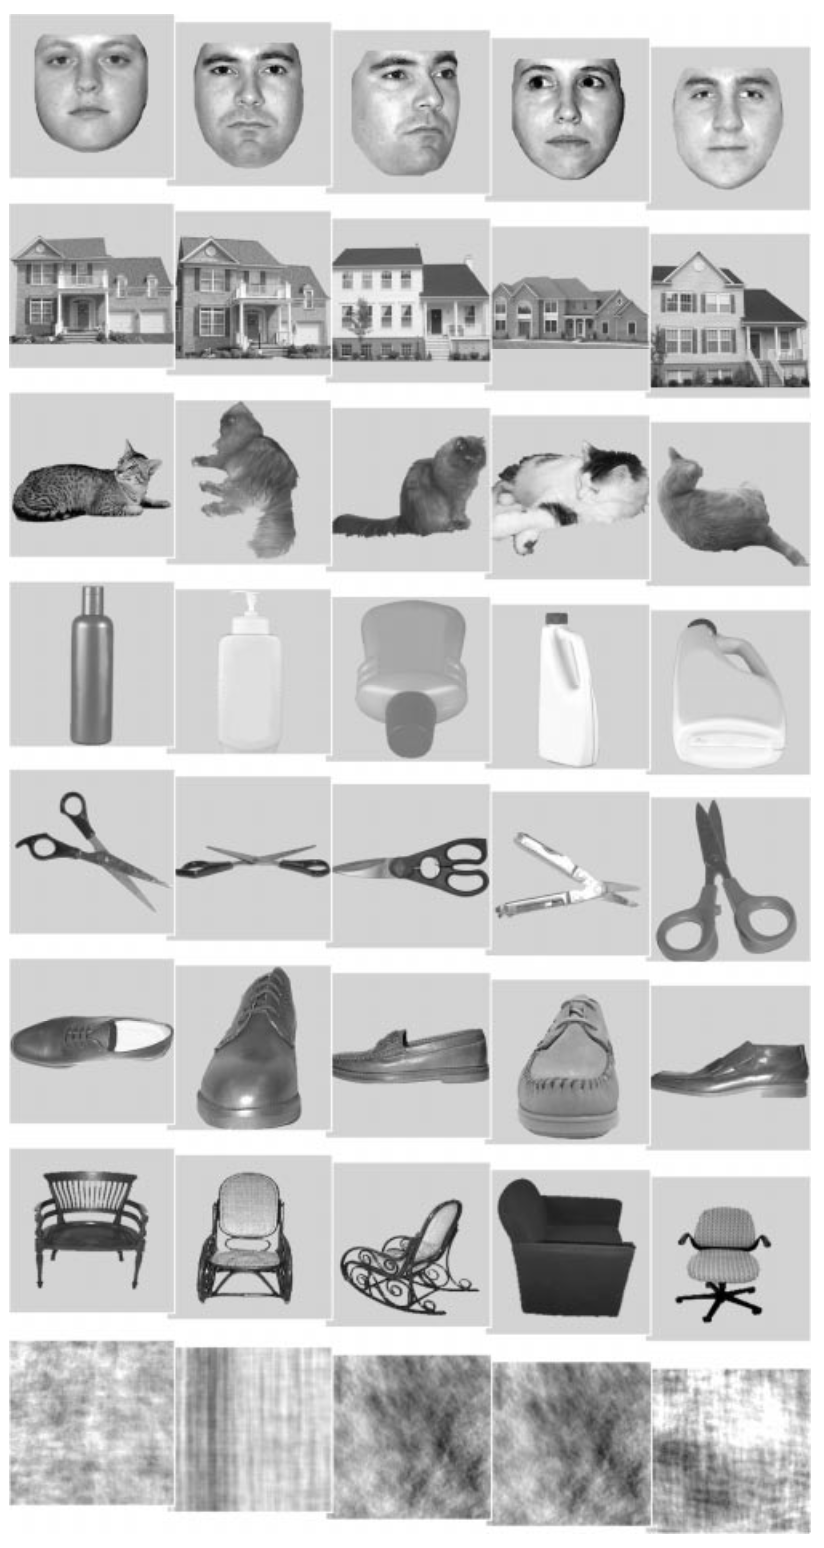
\includegraphics[scale=0.5]{fig/objects_shown.png}
    \caption{Examples of the presented visual categories.}
    \label{fig:objects-shown}
\end{figure}

The experiment had a block structure. Each run contained eight stimulus blocks, with one block corresponding to each visual category. Each block contained 12 image presentations. An image was displayed for $500 \, \mathrm{ms}$ and was followed by a rest interval of $1500 \, \mathrm{ms}$. Therefore, each presentation lasted $2$ seconds, and each category \mbox{block - $24$ seconds}.

The stimulus blocks were separated by $12$-second rest periods. Each run also began and ended with $12$ seconds of rest. Consequently, the complete experimental sequence lasted $300$ seconds.

A total of $96$ images were presented during each run. The same eight categories were included in all $12$ runs, although the order of the category blocks differed. The block structure itself remained unchanged.

\newpage
\subsection{Functional MRI acquisition}
\label{section:fmri-acquisition}

The functional data were acquired using gradient-echo echo-planar imaging (GE-EPI) on a GE 3T scanner. The main acquisition parameters are presented in Table~\ref{tab:acquisition-params}~\cite{MAIN_DATASET}.

\begin{table}[ht]
    \centering
    \begin{threeparttable}
        \begin{tabular}{|c|c|}
            \hline
            Parameter & Value \\
            \hline
            Repetition time, TR & $2500\,\mathrm{ms}$ \\
            Echo time, TE & $30\,\mathrm{ms}$ \\
            Flip angle & $90^\circ$ \\
            Number of slices & $40$ \\
            Slice thickness & $3.5\,\mathrm{mm}$ \\
            Field of view & $24\,\mathrm{cm}$ \\
            Number of time points per run & $121$ \\
            Number of functional runs per participant & $12$\tnote{*} \\
            \hline
        \end{tabular}
        \begin{tablenotes}
            \footnotesize
            \item[*] Subject 5 contains 11 valid functional runs.
        \end{tablenotes}

        \caption{Functional MRI acquisition parameters.}
        \label{tab:acquisition-params}
    \end{threeparttable}
\end{table}

The functional images have spatial dimensions of $40 \times 64 \times 64$. Each run contains 121 time points and covers approximately five minutes of acquisition.

The repetition time of $2500 \, \mathrm{ms}$ means that the BOLD signal is not sampled separately for every individual image presentation, since the images were presented every 2 seconds. The stimulus timing will be convolved with a haemodynamic response function (HRF), further explained in Section~\ref{section:design-matrix}, to model the expected BOLD response \cite{hrf-problems}.

\subsection{Anatomical MRI acquisition}

The dataset also contains one T1-weighted anatomical image for each participant. A T1-weighted image is an anatomical MRI image with higher spatial resolution than the functional MRI images, meaning that it represents brain anatomy using smaller voxels, and therefore provides more detailed structural information \cite{fmri}. This is commonly used as an anatomical reference for registration of functional MRI data \cite{dataset-cit1, MAIN_DATASET}. In the analyzed dataset the images consist of $124$ slices with a slice thickness of $1.2 \, \mathrm{mm}$ and a field of view of $24 \, \mathrm{cm}$. Their spatial dimensions are $124 \times 256 \times 256$.

The anatomical images provide greater spatial detail than the functional images. In this thesis, they are used as an anatomical reference for the visualization of statistical maps. They are not subjected to the denoising methods considered in the thesis.

\section{Organization of the dataset}

The dataset is organized according to the Brain Imaging Data Structure (BIDS) convention~\cite{BIDS}. At the highest level, it contains metadata describing the experiment and separate directories corresponding to individual participants. Each participant directory contains an \verb|anat| directory (T1-weighted anatomical data) and a \verb|func| directory (functional data).

For each participant, except for the subject 5, the \verb|func| directory contains 12 functional BOLD images and 12 corresponding event files. Subject 5 contains 11 of each. Each BOLD file is a four-dimensional image with shape:

\begin{equation}
    \label{eq:init-data-shape}
    X \times Y \times Z \times T,
\end{equation}

where $X$, $Y$, and $Z$ represent the spatial dimensions and $T$ represents the number of time points.

The event files contain the columns \verb|onset|, \verb|duration|, and \verb|trial_type|. The \verb|onset| value gives the time of a stimulus presentation in seconds relative to the beginning of the corresponding run. The \verb|duration| value specifies how long the stimulus was displayed, while \verb|trial_type| identifies its category.

\section{Caveats related to the dataset}
\label{section:caveats}

The experimental conditions were repeated across 12 runs. This makes leave-one-run-out cross-validation possible. For a single cross-validation fold, the 12 runs are split into two datasets:
\begin{enumerate}
    \item training dataset, consisting of 11 runs;
    \item test dataset, consisting of the left-out run.
\end{enumerate}
For each fold, data from one run are used as a test dataset, until data from all 12 runs are used as a test dataset, i.e., left-out run. 12 runs means 12 cross-validation folds. This allows the predictive performance of the fitted model to be evaluated on data not used during estimation \cite{glm-denoise}. The multiple-run structure may also help identify run-specific noise effects. The detailed description and implementation of this framework will be explained in the later chapters.

The dataset does not provide a noise-free reference image or a known true BOLD signal. The quality of denoising must therefore be evaluated indirectly using criteria such as:
\begin{itemize}
    \item prediction accuracy, measured using the coefficient of determination $R^2$ \cite{coefficient-determination};
    \item stability of the estimated task-related coefficients \cite{jackknife};
    \item spatial distributions of the estimated task-related coefficients, visualized using beta maps \cite{spm-filter};
    \item spatial patterns of task-related effects, evaluated using contrast $t$-maps \cite{tmaps}.
\end{itemize}

The dataset also has several limitations. It contains only six participants and was acquired using an older method with relatively coarse spatial and temporal resolution. It represents one specific visual experiment with a block design. Therefore, conclusions obtained using this dataset may not generalize directly to other conditions, such as event-related designs, resting-state data, or experiments involving different processes. Furthermore, as described in Subsection~\ref{section:dataset-description}, subject 5 has only 11 valid functional runs. Consequently, analyses based on leave-one-run-out cross-validation use 11 folds for this subject instead of 12. Lastly, the dataset does not include separate respiratory or cardiac recordings often provided in the BIDS structure \cite{BIDS}, which could be used to construct physiological nuisance regressors. 

Nevertheless, the repeated and clearly defined experimental structure makes the dataset useful for comparing denoising methods. In particular, the presence of multiple repeated runs per participant supports within-subject cross-validation and the evaluation of the stability of task-related estimates.

\newpage
\chapter{General Linear Model}
\label{chapter:glm}

The first model is the General Linear Model (GLM). It is viewed as a special case of the Generalized Linear Model with a Gaussian response distribution and the identity link function, defined in \cite[Section 1.1.4]{agresti} as Linear Model. However, the name General Linear Model is conventionally used in the fMRI literature \cite{spm-filter}.

The notation and standard regression derivations presented in Sections~\ref{section:model-definition}, \ref{section:ols-estimation}, and \ref{section:gls-prewhitening} follow the treatment given by \cite{agresti}.

\section{Model definition}
\label{section:model-definition}

In general, for a single voxel in fMRI, the GLM can be written as

\begin{equation}
    \mathbf{y} = \mathbf{X}\boldsymbol{\beta} + \boldsymbol{\varepsilon},
\end{equation}

where

\begin{itemize}
    \item $\mathbf{y} \in \mathbb{R}^{t}$ contains the observed BOLD signal for a given voxel over $t$ time points;
    \item $\mathbf{X} \in \mathbb{R}^{t \times p}$ is the design matrix;
    \item $\boldsymbol{\beta} \in \mathbb{R}^{p}$ contains the unknown regression coefficients;
    \item $\boldsymbol{\varepsilon} \in \mathbb{R}^{t}$ is the error vector.
\end{itemize}

Each column of $\mathbf{X}$ represents a task-related effect or another modeled source of variability. The corresponding element of $\boldsymbol{\beta}$ describes the estimated contribution of that regressor to the BOLD time series at the considered voxel. In voxelwise fMRI analysis, the same design matrix is typically used for all voxels, while a separate coefficient vector is estimated for each voxel.

Equivalently, the models for all voxels can be written simultaneously as $\mathbf{Y} = \mathbf{X} \mathbf{B} + \mathbf{E}$, where each column of $\mathbf{Y}$ contains the time series of one voxel. As an example, consider a simple data matrix and design matrix:

\begin{equation}
    \mathbf{Y} = 
    \begin{bmatrix}
        y_{11} & y_{12} \\
        y_{21} & y_{22} \\
        y_{31} & y_{32}
    \end{bmatrix}
    =
    \begin{bmatrix}
        \mathbf{y}_1 & \mathbf{y}_2
    \end{bmatrix}, \qquad
    \mathbf{X} =
    \begin{bmatrix}
        x_{11} & x_{12} \\
        x_{21} & x_{22} \\
        x_{31} & x_{32}
    \end{bmatrix}.
\end{equation}

\newpage
Let 

\begin{equation}
    \mathbf{B} = 
    \begin{bmatrix}
        \beta_{11} & \beta_{12} \\
        \beta_{21} & \beta_{22} \\
    \end{bmatrix}
    = 
    \begin{bmatrix}
        \boldsymbol{\beta}_1 & \boldsymbol{\beta}_2
    \end{bmatrix}
    , \qquad
    \mathbf{E} = 
    \begin{bmatrix}
        \varepsilon_{11} & \varepsilon_{12} \\
        \varepsilon_{21} & \varepsilon_{22} \\
        \varepsilon_{31} & \varepsilon_{32} \\
    \end{bmatrix}
    = 
    \begin{bmatrix}
        \boldsymbol{\varepsilon}_1 & \boldsymbol{\varepsilon}_2
    \end{bmatrix}
\end{equation}

be the matrix of regression coefficients and the matrix of error terms, respectively. It is not hard to see, that such a matrix system $\mathbf{Y} = \mathbf{X}\mathbf{B} + \mathbf{E}$ can be written as two separate systems:

\begin{equation}
    \begin{aligned}
        \mathbf{y}_1 &= \mathbf{X}\boldsymbol{\beta}_1 + \boldsymbol{\varepsilon}_1, \\
        \mathbf{y}_2 &= \mathbf{X}\boldsymbol{\beta}_2 + \boldsymbol{\varepsilon}_2. \\
    \end{aligned}
\end{equation}

Furthermore, this example illustrates how the same design matrix $\mathbf{X}$ is used for every voxel, while each voxel has its own regression coefficient vector and error vector.

\section{Ordinary Least Squares estimation}
\label{section:ols-estimation}

The Ordinary Least Squares (OLS) estimator is obtained by minimizing the objective function $L$, which is equal to the squared Euclidean norm of the residual vector 
\newline
\cite[Section~2.1]{agresti}:

\begin{align}
    L(\boldsymbol{\beta}) &= \left\lVert\mathbf{y}-\mathbf{X}\boldsymbol{\beta}\right\rVert_2^2 \\
    &= \left(\mathbf{y}-\mathbf{X}\boldsymbol{\beta}\right)^T \left(\mathbf{y}-\mathbf{X}\boldsymbol{\beta}\right) \\
    &= \mathbf{y}^T\mathbf{y} - 2\mathbf{y}^T\mathbf{X}\boldsymbol{\beta} + \boldsymbol{\beta}^T \mathbf{X}^T\mathbf{X} \boldsymbol{\beta}.
\end{align}

To minimize this function, its derivative with respect to $\boldsymbol{\beta}$ is set equal to zero:

\begin{equation}
    \frac{\partial L(\boldsymbol{\beta})}{\partial \boldsymbol{\beta}} = -2\mathbf{X}^T \left( \mathbf{y}-\mathbf{X}\boldsymbol{\beta} \right).
\end{equation}

For the estimator $\widehat{\boldsymbol{\beta}}$, this gives the normal equations \cite[equation~2.2]{agresti}

\begin{equation}
    \mathbf{X}^T\mathbf{y} = \mathbf{X}^T\mathbf{X} \widehat{\boldsymbol{\beta}}.
\end{equation}

If $\mathbf{X}$ has full column rank $p$, then $\mathbf{X}^T\mathbf{X}$ is invertible and the OLS estimator 
\newline
is~\mbox{\cite[equation~2.3]{agresti}}

\begin{equation}
    \widehat{\boldsymbol{\beta}}_{\mathrm{OLS}} = \left(\mathbf{X}^T\mathbf{X}\right)^{-1} \mathbf{X}^T\mathbf{y}.
    \label{eq:ols-estimator}
\end{equation}

The fitted values are then given by

\begin{align}
    \widehat{\mathbf{y}} &= \mathbf{X}\widehat{\boldsymbol{\beta}}_{\mathrm{OLS}} \\
    &= \mathbf{X} \left(\mathbf{X}^T\mathbf{X}\right)^{-1}\mathbf{X}^T\mathbf{y}.
\end{align}

We can construct the hat matrix, which describes the transformation $\widehat{\mathbf{y}} = \mathbf{H}\mathbf{y}$:

\begin{equation}
    \mathbf{H} = \mathbf{X} \left(\mathbf{X}^T\mathbf{X}\right)^{-1}\mathbf{X}^T.
    \label{eq:hat-matrix}
\end{equation}

Geometrically, the hat matrix also projects the vector $\mathbf{y}$ orthogonally onto the column space spanned by $\mathbf{X}$, thus $\mathbf{H}$ is called a projection matrix \cite{hat-matrix}.

The residual vector is therefore

\begin{align}
    \label{eq:ols-residuals}
    \mathbf{e} &= \mathbf{y}-\widehat{\mathbf{y}} \\
    &= \mathbf{y}-\mathbf{H}\mathbf{y} \\
    &= \left(\mathbf{I}-\mathbf{H}\right)\mathbf{y}.
    \label{eq:ols-residuals-hat}
\end{align}

Because

\begin{equation}
    \begin{aligned}
        \left(\mathbf{I}-\mathbf{H}\right)\mathbf{X} &= \left(\mathbf{I}- \mathbf{X} \left(\mathbf{X}^T\mathbf{X}\right)^{-1}\mathbf{X}^T\right)\mathbf{X} \\
        &= \left(\mathbf{X}- \mathbf{X} \left(\mathbf{X}^T\mathbf{X}\right)^{-1}\mathbf{X}^T\mathbf{X}\right) \\
        &= \left(\mathbf{X}- \mathbf{X} \left(\mathbf{X}^T\mathbf{X}\right)^{-1}\left(\mathbf{X}^T\mathbf{X}\right)\right) \\
        &= \left(\mathbf{X}- \mathbf{X} \mathbf{I}\right) = \mathbf{0}, \\
    \end{aligned}
    \label{eq:hat-zeroing}
\end{equation}

the residual vector in Equation~\eqref{eq:ols-residuals-hat} can also be written as

\begin{equation}
    \mathbf{e} = (\mathbf{I}-\mathbf{H}) (\mathbf{X}\boldsymbol{\beta} + \boldsymbol{\varepsilon}) = (\mathbf{I}-\mathbf{H})\boldsymbol{\varepsilon}.
\end{equation}

The fitted values and residuals do not by themselves define the denoised fMRI signal. For denoising, the columns of the design matrix must first be divided into task-related and nuisance regressors. The estimated nuisance contribution can then be subtracted from the observed signal. This procedure, together with the construction of the design matrix, will be described in the later sections.

\section{Generalized Least Squares and prewhitening}
\label{section:gls-prewhitening}

Under the classical linear model assumptions, the error vector has zero mean, constant variance, and uncorrelated components \cite[Section 2.2]{agresti}:

\begin{equation}
    \mathbb{E}(\boldsymbol{\varepsilon}) = \mathbf{0},
    \qquad
    \operatorname{Var}(\boldsymbol{\varepsilon}) = \sigma^2\mathbf{I}.
\end{equation}

This assumption is generally not possible for fMRI time series. Measurements from the same voxel at consecutive time points are commonly autocorrelated. Therefore, the covariance matrix of the errors may have a more general form \cite[Section 2.7.2]{agresti}:

\begin{equation}
    \operatorname{Var}(\boldsymbol{\varepsilon}) = \sigma^2\mathbf{V},
    \label{eq:general-error-covariance}
\end{equation}

where $\mathbf{V}$ describes the correlation structure and does not have to be the identity matrix.

Suppose that $\mathbf{X}$ has full column rank and $\mathbf{V}$ is a known, positive definite matrix. The spectral decomposition of $\mathbf{V}$ is

\begin{equation}
    \mathbf{V} = \mathbf{Q}\boldsymbol{\Lambda}\mathbf{Q}^T,
\end{equation}

where $\boldsymbol{\Lambda}$ is a diagonal matrix containing the positive eigenvalues of $\mathbf{V}$, while $\mathbf{Q}$ is an orthogonal matrix whose columns are the corresponding eigenvectors \cite[Section 2.7.2]{agresti}:

\begin{equation}
    \mathbf{Q}^T\mathbf{Q} = \mathbf{Q}\mathbf{Q}^T = \mathbf{I}.
\end{equation}

\newpage

The symmetric square root and inverse square root of $\mathbf{V}$ can therefore be defined as

\begin{align}
    \mathbf{V}^{1/2} &= \mathbf{Q}\boldsymbol{\Lambda}^{1/2}\mathbf{Q}^T, \\
    \mathbf{V}^{-1/2} &= \mathbf{Q}\boldsymbol{\Lambda}^{-1/2}\mathbf{Q}^T.
\end{align}

The transformed variables are defined as

\begin{equation}
    \mathbf{y}^{\ast} = \mathbf{V}^{-1/2}\mathbf{y}, \qquad \mathbf{X}^{\ast} = \mathbf{V}^{-1/2}\mathbf{X}, \qquad \boldsymbol{\varepsilon}^{\ast} = \mathbf{V}^{-1/2}\boldsymbol{\varepsilon},
    \label{eq:prewhitening-transform}
\end{equation}

therefore, the transformed model is

\begin{equation}
    \mathbf{y}^{\ast} = \mathbf{X}^{\ast}\boldsymbol{\beta} + \boldsymbol{\varepsilon}^{\ast}.
\end{equation}

Its expected value is

\begin{equation}
    \begin{aligned}
        \mathbb{E}\left(\mathbf{y}^{\ast}\right) &= \mathbb{E}\left(\mathbf{V}^{-1/2}\mathbf{y}\right) \\
        &= \mathbf{V}^{-1/2}\mathbf{X}\boldsymbol{\beta} \\
        &= \mathbf{X}^{\ast}\boldsymbol{\beta},
    \end{aligned}
\end{equation}

while the covariance matrix of the transformed errors is

\begin{equation}
    \begin{aligned}
        \operatorname{Var}\left(\boldsymbol{\varepsilon}^{\ast}\right) &= \operatorname{Var}\left( \mathbf{V}^{-1/2}\boldsymbol{\varepsilon} \right) \\
        &= \mathbf{V}^{-1/2} \operatorname{Var}(\boldsymbol{\varepsilon}) \left( \mathbf{V}^{-1/2} \right)^T \\
        &= \mathbf{V}^{-1/2} \sigma^2\mathbf{V} \left(\mathbf{V}^{-1/2}\right)^T \\
        &= \sigma^2\ \mathbf{V}^{-1/2} \mathbf{V} \mathbf{V}^{-1/2} \\
        &= \sigma^2\ \mathbf{V}^{-1/2} \mathbf{V}^{1/2} \mathbf{V}^{1/2} \mathbf{V}^{-1/2} \\
        &= \sigma^2\mathbf{I}.
    \end{aligned}
\end{equation}

Thus, the transformed errors are uncorrelated and have equal variance. OLS can therefore be applied to the transformed model. This gives

\begin{equation}
    \begin{aligned}
        \widehat{\boldsymbol{\beta}}_{\mathrm{GLS}} 
        &= \left[ \left( \mathbf{X}^{\ast} \right)^T \mathbf{X}^{\ast} \right]^{-1} \left( \mathbf{X}^{\ast} \right)^T \mathbf{y}^{\ast} \\
        &= \left[ \left( \mathbf{V}^{-1/2} \mathbf{X} \right)^T \mathbf{V}^{-1/2} \mathbf{X} \right]^{-1} \left( \mathbf{V}^{-1/2} \mathbf{X} \right)^T \mathbf{V}^{-1/2} \mathbf{y} \\
        &= \left[  \mathbf{X}^T \mathbf{V}^{-1/2} \mathbf{V}^{-1/2} \mathbf{X} \right]^{-1} \mathbf{X}^T \mathbf{V}^{-1/2} \mathbf{V}^{-1/2} \mathbf{y} \\
        &= \left( \mathbf{X}^T \mathbf{V}^{-1} \mathbf{X} \right)^{-1} \mathbf{X}^T \mathbf{V}^{-1} \mathbf{y}.
    \end{aligned}
    \label{eq:gls-estimator}
\end{equation}

This is the Generalized Least Squares (GLS) estimator of $\boldsymbol{\beta}$ \cite[Equation 2.12]{agresti}. The transformation of the data and design matrix by $\mathbf{V}^{-1/2}$ is referred to as \textit{prewhitening}. The term was coined in \cite[p. 215]{prewhitening} and refers to a transformation that removes the covariance structure so that the transformed errors have a white-noise covariance structure. Below are the definitions of both a \textit{white} random vector and \textit{prewhitening}, which follow the terminology used in \cite{ica}. 

\newpage
\begin{definition}[White random vector]
A random vector $\mathbf{z} = \begin{bmatrix}z_1 & z_2 & \ldots & z_n\end{bmatrix}^T$ is said to be white or sphered if it is centered

$$ \mathbb{E}[\mathbf{z}] = \mathbf{0}, $$

and its elements are uncorrelated and have unit variances

$$ \operatorname{Cov}(\mathbf{z}) = \mathbb{E}\left[\mathbf{z}\mathbf{z}^T\right] = \mathbf{I} $$
\end{definition}

\begin{definition}[Prewhitening]
\label{def:prewhitening}
Let $\mathbf{x}$ be a centered random vector with covariance matrix

$$ \boldsymbol{\Sigma} = \mathbf{E}\mathbf{D}\mathbf{E}^T, $$

where $\mathbf{E}$ contains the eigenvectors of $\boldsymbol{\Sigma}$
and $\mathbf{D}$ is the diagonal matrix of corresponding eigenvalues.

The whitening or prewhitening procedure is the transformation of the vector $\mathbf{x}$ into a white vector $\mathbf{z}$:
$$ \mathbf{z} = \mathbf{D}^{-1/2}\mathbf{E}^T\mathbf{x}, $$

such that

$$ \operatorname{Cov}(\mathbf{z}) = \mathbf{I}. $$
\end{definition}

If the covariance structure $\mathbf{V}$ is correctly specified and known, GLS provides the Best Linear Unbiased Estimator (BLUE) of the regression coefficients \cite{agresti, woolrich-temporal-autocorrelation, bullmore-fmri-estimation}.

In practice, $\mathbf{V}$ is unknown and must be estimated from the data. From this, the resulting procedure is described as Feasible Generalized Least Squares (FGLS) \cite{fgls}. The estimation of the \textit{temporal covariance} structure, including its possible autoregressive representation, is discussed in Section~\ref{section:ar-noise-model}. Here, temporal covariance refers to the covariance between regression errors at different time points.


\section{Autoregressive temporal-noise model}
\label{section:ar-noise-model}

As mentioned in Section~\ref{section:gls-prewhitening}, the assumption of uncorrelated errors is generally not~appropriate for fMRI time series. This creates the need for the covariance matrix $\mathbf{V}$ introduced in Equation~\eqref{eq:general-error-covariance}. Since $\mathbf{V}$ is unknown, it must be estimated from the observed data
\newline
\cite[Section 2.7.3]{agresti}.

In time-series data, the regression errors are unlikely to be independent, especially in fMRI data. In this thesis, they are assumed to be a stationary process. Stationarity means that the mean and variance of the error process are constant over time, while the covariance between two errors depends on their temporal lag. Additionally, assume mean centered errors

\begin{equation}
    \mathbb{E}\left[\varepsilon_t\right] = 0, \qquad \operatorname{Var}\left[\varepsilon_t\right] = \gamma(0) = \sigma_\varepsilon^2,
\end{equation}

and

\begin{equation} 
    \operatorname{Cov} \left[\varepsilon_t, \varepsilon_{t+s} \right] = \gamma(s), \qquad \rho(s) = \frac{\gamma(s)}{\gamma(0)}, \qquad s \in \mathbb{Z}
\end{equation}

where $\gamma(s)$ is the autocovariance function and $\rho(s)$ is the autocorrelation function at lag $s$.

The covariance matrix of the error vector can then be written as

\begin{equation}
    \boldsymbol{\Sigma} = \sigma_\varepsilon^2\mathbf{V}, \qquad V_{ij} = \rho(|i-j|).
\end{equation}

Thus, $\mathbf{V}$ is the temporal correlation matrix, while $\boldsymbol{\Sigma}$ is the corresponding covariance matrix.

A simple model for temporally autocorrelated regression errors is the first-order autoregressive process \cite{ols-ar-connection}, denoted by AR(1):

\begin{equation}
    \varepsilon_t = \phi\varepsilon_{t-1} + \nu_t, \qquad \nu_t \overset{\mathrm{i.i.d.}}{\sim} \mathcal{N} \left(0, \sigma_\nu^2 \right), \qquad t \in \mathbb{Z}
\end{equation}

where $\phi$ is the autoregressive coefficient and $\nu_t$ is the noise term.

For the AR(1) process to be stationary, the autoregressive coefficient must satisfy 

\begin{equation}
    |\phi| < 1.
\end{equation}

Under this condition, the variance and autocorrelation function are \cite{ols-ar-connection}

\begin{equation}
    \sigma_\varepsilon^2 = \frac{\sigma_\nu^2}{1-\phi^2}, \qquad \rho(s) = \phi^{|s|}.
\end{equation}

In particular, the correlation between two one-lagged errors is

\begin{equation}
    \rho(1)=\phi
\end{equation}

and, crucially, the magnitude of the autocorrelation decreases geometrically with~the~lag

\begin{equation}
    \rho(s) \longrightarrow 0 \quad \text{as } |s|\longrightarrow\infty.
\end{equation}

The temporal correlation matrix therefore has the form

\begin{equation}
    V_{ij} = \phi^{|i-j|}.
\end{equation}

Since the true regression errors $\boldsymbol{\varepsilon}$ are not observed, the autoregressive coefficient must be estimated from residuals obtained from an initial OLS model fit, introduced in Equation~\eqref{eq:ols-residuals}:

\begin{equation}
    \mathbf{e} = \mathbf{y}-\widehat{\mathbf{y}} = \mathbf{y} - \mathbf{X}\widehat{\boldsymbol{\beta}}_{\mathrm{OLS}}
\end{equation}

In order to estimate the autoregressive parameter $\phi$ we can fit the AR(1) equation using OLS, treating $e_t$ as the response and $e_{t-1}$ as the predictor. The next step is therefore to minimize:
\begin{equation}
    L(\phi) = \sum_{t=2}^{n} (e_t - \phi e_{t-1})^2,
\end{equation}

finally obtaining

\begin{equation}
    \widehat{\phi} = \frac{\sum_{t=2}^{n} e_t e_{t-1} }{\sum_{t=2}^{n}e_{t-1}^2}.
    \label{eq:phi-estimation}
\end{equation}

\newpage
The estimated temporal correlation matrix is then constructed from the estimated autoregressive parameter

\begin{equation}
    \widehat{V}_{ij} = \widehat{\phi}^{|i-j|}.
    \label{eq:estimated-ar1-covariance}
\end{equation}

There are several ways in which a covariance matrix can be further constructed for the fMRI data. In this thesis, the choice was made to estimate one covariance matrix per run. This choice requires a single value of $\phi$ for each run. Rather than estimating this parameter jointly across all voxels, $\phi$ is first estimated separately for each voxel using Equation~\eqref{eq:phi-estimation}. The median of the resulting voxelwise estimates is then used to construct the run-specific correlation matrix $\widehat{\mathbf V}$. This matrix can now be used in the prewhitening transformation from Equation~\eqref{eq:prewhitening-transform}:

\begin{equation}
    \mathbf{y}^{\ast} = \widehat{\mathbf{V}}^{-1/2}\mathbf{y}, \qquad \mathbf{X}^{\ast} = \widehat{\mathbf{V}}^{-1/2}\mathbf{X}.
\end{equation}

The regression model is then fitted again using the transformed data, as described in Section~\ref{section:gls-prewhitening}.


\section{Construction of the design matrix}
\label{section:design-matrix}

The construction of the design matrix is a crucial part of GLM-based denoising. The design matrix contains explanatory variables representing task-related and nuisance variability. The estimated coefficients of the task-related regressors are used to model the BOLD response associated with the experiment, while the coefficients of the nuisance regressors describe contribution of modeled nuisance effects.

For a single voxel, the GLM can be written as

\begin{equation}
    \mathbf{y} = \mathbf{X}_{\mathrm{task}} \boldsymbol{\beta}_{\mathrm{task}} + \mathbf{X}_{\mathrm{nuis}} \boldsymbol{\beta}_{\mathrm{nuis}} + \boldsymbol{\varepsilon},
\end{equation}

where the design matrix and coefficient vector are partitioned as

\begin{equation}
    \mathbf{X} =
    \begin{bmatrix}
        \mathbf{X}_{\mathrm{task}} & \mathbf{X}_{\mathrm{nuis}}
    \end{bmatrix},
    \qquad
    \boldsymbol{\beta} =
    \begin{bmatrix}
        \boldsymbol{\beta}_{\mathrm{task}} \\
        \boldsymbol{\beta}_{\mathrm{nuis}}
    \end{bmatrix}.
\end{equation}

After fitting the model, the estimated nuisance contribution is

\begin{equation}
    \widehat{\mathbf{y}}_{\mathrm{nuis}} = \mathbf{X}_{\mathrm{nuis}} \widehat{\boldsymbol{\beta}}_{\mathrm{nuis}}.
\end{equation}

The denoised time series can then be defined by subtracting this contribution from the observed signal:

\begin{equation}
    \mathbf{y}_{\mathrm{denoised}} = \mathbf{y} - \widehat{\mathbf{y}}_{\mathrm{nuis}}.
    \label{eq:glm-denoised-signal}
\end{equation}

This procedure removes only the contribution assigned to nuisance regressors, while the fitted task-related component is not subtracted from the data.

A typical fMRI design matrix can contain task-related regressors, motion regressors, physiological regressors, drift regressors, and data-derived nuisance regressors.

For a given run, the untransformed design matrix is the same for all analyzed voxels. Each voxel has its own estimated coefficient vector. Separate design matrices are constructed for different runs because stimulus timing and run-specific nuisance effects may differ between them.

\subsection{Task-related regressors}
\label{section:task-regressors}

As described in Subsection~\ref{section:experiment}, the participants were presented with visual stimuli at specified times during each experimental run. The purpose of the task-related regressors is to model the expected BOLD response associated with these stimulus presentations.

The event files provided with the dataset contain the onset, duration, and category of each stimulus. The stimuli belong to eight visual categories, further described in Subsection~\ref{section:experiment}. Therefore, the task-related part of the design matrix contains eight columns, with one column corresponding to each category:

\begin{equation}
    \mathbf{X}_{\mathrm{task}} \in \mathbb{R}^{n \times 8},
\end{equation}

where $n$ is the number of data points in each run.

In the analyzed dataset, each category is presented 12 times within its block. Each individual image is displayed for $0.5$ seconds and is followed by a $1.5$-second break. In the model, each image presentation together with the following interstimulus interval is represented by a $2$-second boxcar function. Since consecutive presentations occur every $2$ seconds, the twelve boxcar functions represent the full $24$-second category block.

A boxcar function is a binary function that takes the value one during the modeled interval and zero otherwise:

\begin{equation}
    \operatorname{boxcar}(t; A,d)
    := \mathbbm{1}_{[A,A+d)}(t)
    =
    \begin{cases}
        1, & t \in [A,A+d),\\
        0, & \text{otherwise}.
    \end{cases}
\end{equation}

An example of such a function is shown on the first plot in Figure~\ref{fig:hrf-boxcar-convolution}, where the function is active from $15$ to $20$ seconds.

For category $k$, let $J_k$ denote the number of stimulus presentations, and let $o_{kj}$ and $d_{kj}$ denote the onset and duration of the $j$-th presentation interval, respectively. The stimulus is then

\begin{equation}
    s_k(t) = \sum_{j=1}^{J_k} \mathbbm{1}_{[o_{kj},\,o_{kj}+d_{kj})}(t).
    \label{eq:stimulus-function}
\end{equation}

The set of categories is the same for every run, but the order of the category blocks differs. As a result, the eight columns have the same interpretation across runs, but their temporal profiles differ between runs.

\subsubsection{Haemodynamic response function}

The stimulus functions describe when the stimuli were presented, but they do not directly represent the expected BOLD response. The actual haemodynamic response is delayed and temporally dispersed relative to the neural event currently taking place. Therefore, each stimulus function is convolved with a haemodynamic response function (HRF) \cite{hrf-theory}.

The task regressor for category $k$ is defined as \cite[Equation 1]{hrf-theory}

\begin{equation}
    x_k(t) = \left(s_k \ast h\right)(t) + \eta(t)
\end{equation}

where
\begin{enumerate}
    \item $h$ denotes the selected HRF;
    \item $\eta$ denotes the noise of the measurement.
\end{enumerate}

Since the objective is to model the clean BOLD signal in this regressor, the noise measurement will not be present, i.e., $\eta \equiv 0$, and instead will be present in the nuisance regressors and residuals.

The HRF describes the expected haemodynamic response following a short neural event. Its shape can be characterized by quantities such as its peak amplitude, time-to-peak, and full-width at half-maximum. A correctly modeled HRF should have its parameters reflect these key components of the haemodynamic response \cite{hrf-problems}:
\begin{itemize}
    \item \textit{amplitude}: magnitude of the BOLD response,
    \item \textit{time-to-peak}: latency of the response to the stimulus,
    \item \textit{full-width at half-maximum}: duration of neural activity.
\end{itemize}

Importantly, the relationship between neural activity and the measured BOLD response is not exact. Neural responses vary across presentations, while the HRF differs between participants, brain regions, and experimental conditions. The BOLD signal is also an indirect and delayed reponse to neural activity. A fixed HRF may therefore differ from the true response present in the data \cite{hrf-problems}.

Several approaches can be used to model the HRF. Additional basis functions or estimated HRF parameters provide greater flexibility, but they also increase the number of parameters, reduce the available residual degrees of freedom, and may increase the variance of the estimated coefficients \cite{hrf-problems}. To keep the model consistent across runs and methods, this thesis uses a single canonical HRF.

The selected function is the canonical HRF used in Statistical Parameter Mapping (SPM). A representation of this function is a difference of two gamma density functions \cite[Equation A1]{hrf-problems}:

\begin{equation}
    h(t) = g(t;\alpha_1,\theta_1) - cg(t;\alpha_2,\theta_2),
\end{equation}

where

\begin{equation}
    g(t;\alpha,\theta) = \frac{t^{\alpha-1}e^{-t/\theta}}{\Gamma(\alpha)\theta^\alpha}.
\end{equation}

The authors of \cite{hrf-problems} use the following parameters: 

\begin{equation}
    \alpha_1 = 6, \qquad \alpha_2 = 16, \qquad \theta_1 = \theta_2 = 1, \qquad c = \frac{1}{6}.
    \label{eq:fixed-paramters}
\end{equation}

The component $g(t; \alpha_1, \theta_1)$ represents the main positive haemodynamic response, visible on the second plot of Figure~\ref{fig:hrf-boxcar-convolution} during approximately the first 12 seconds. The component $cg(t; \alpha_2, \theta_2)$ represents the post-stimulus undershoot, which can be seen on the same plot over a period from approximately 12 to 25 seconds. In this thesis, the choice was made to use the fixed parameters presented in Equation~\eqref{eq:fixed-paramters}, rather than estimate them separately from the analyzed data. 

For a fixed scaling convention, the HRF is normalized to have a maximum value of one:

\begin{equation}
    \widetilde{h}(t) = \frac{h(t)}{\max_{\tau \geq 0} h(\tau)}.
\end{equation}

This normalization fixes the scale of the HRF and affects the interpretation of the corresponding regression coefficients. It does not change the shape of the regressor.

The same HRF convolution is performed for each visual category. An example showing the stimulus function, canonical HRF, and the resulting convolved task regressor is presented in Figure~\ref{fig:hrf-boxcar-convolution}.

\begin{figure}[ht]
    \centering
    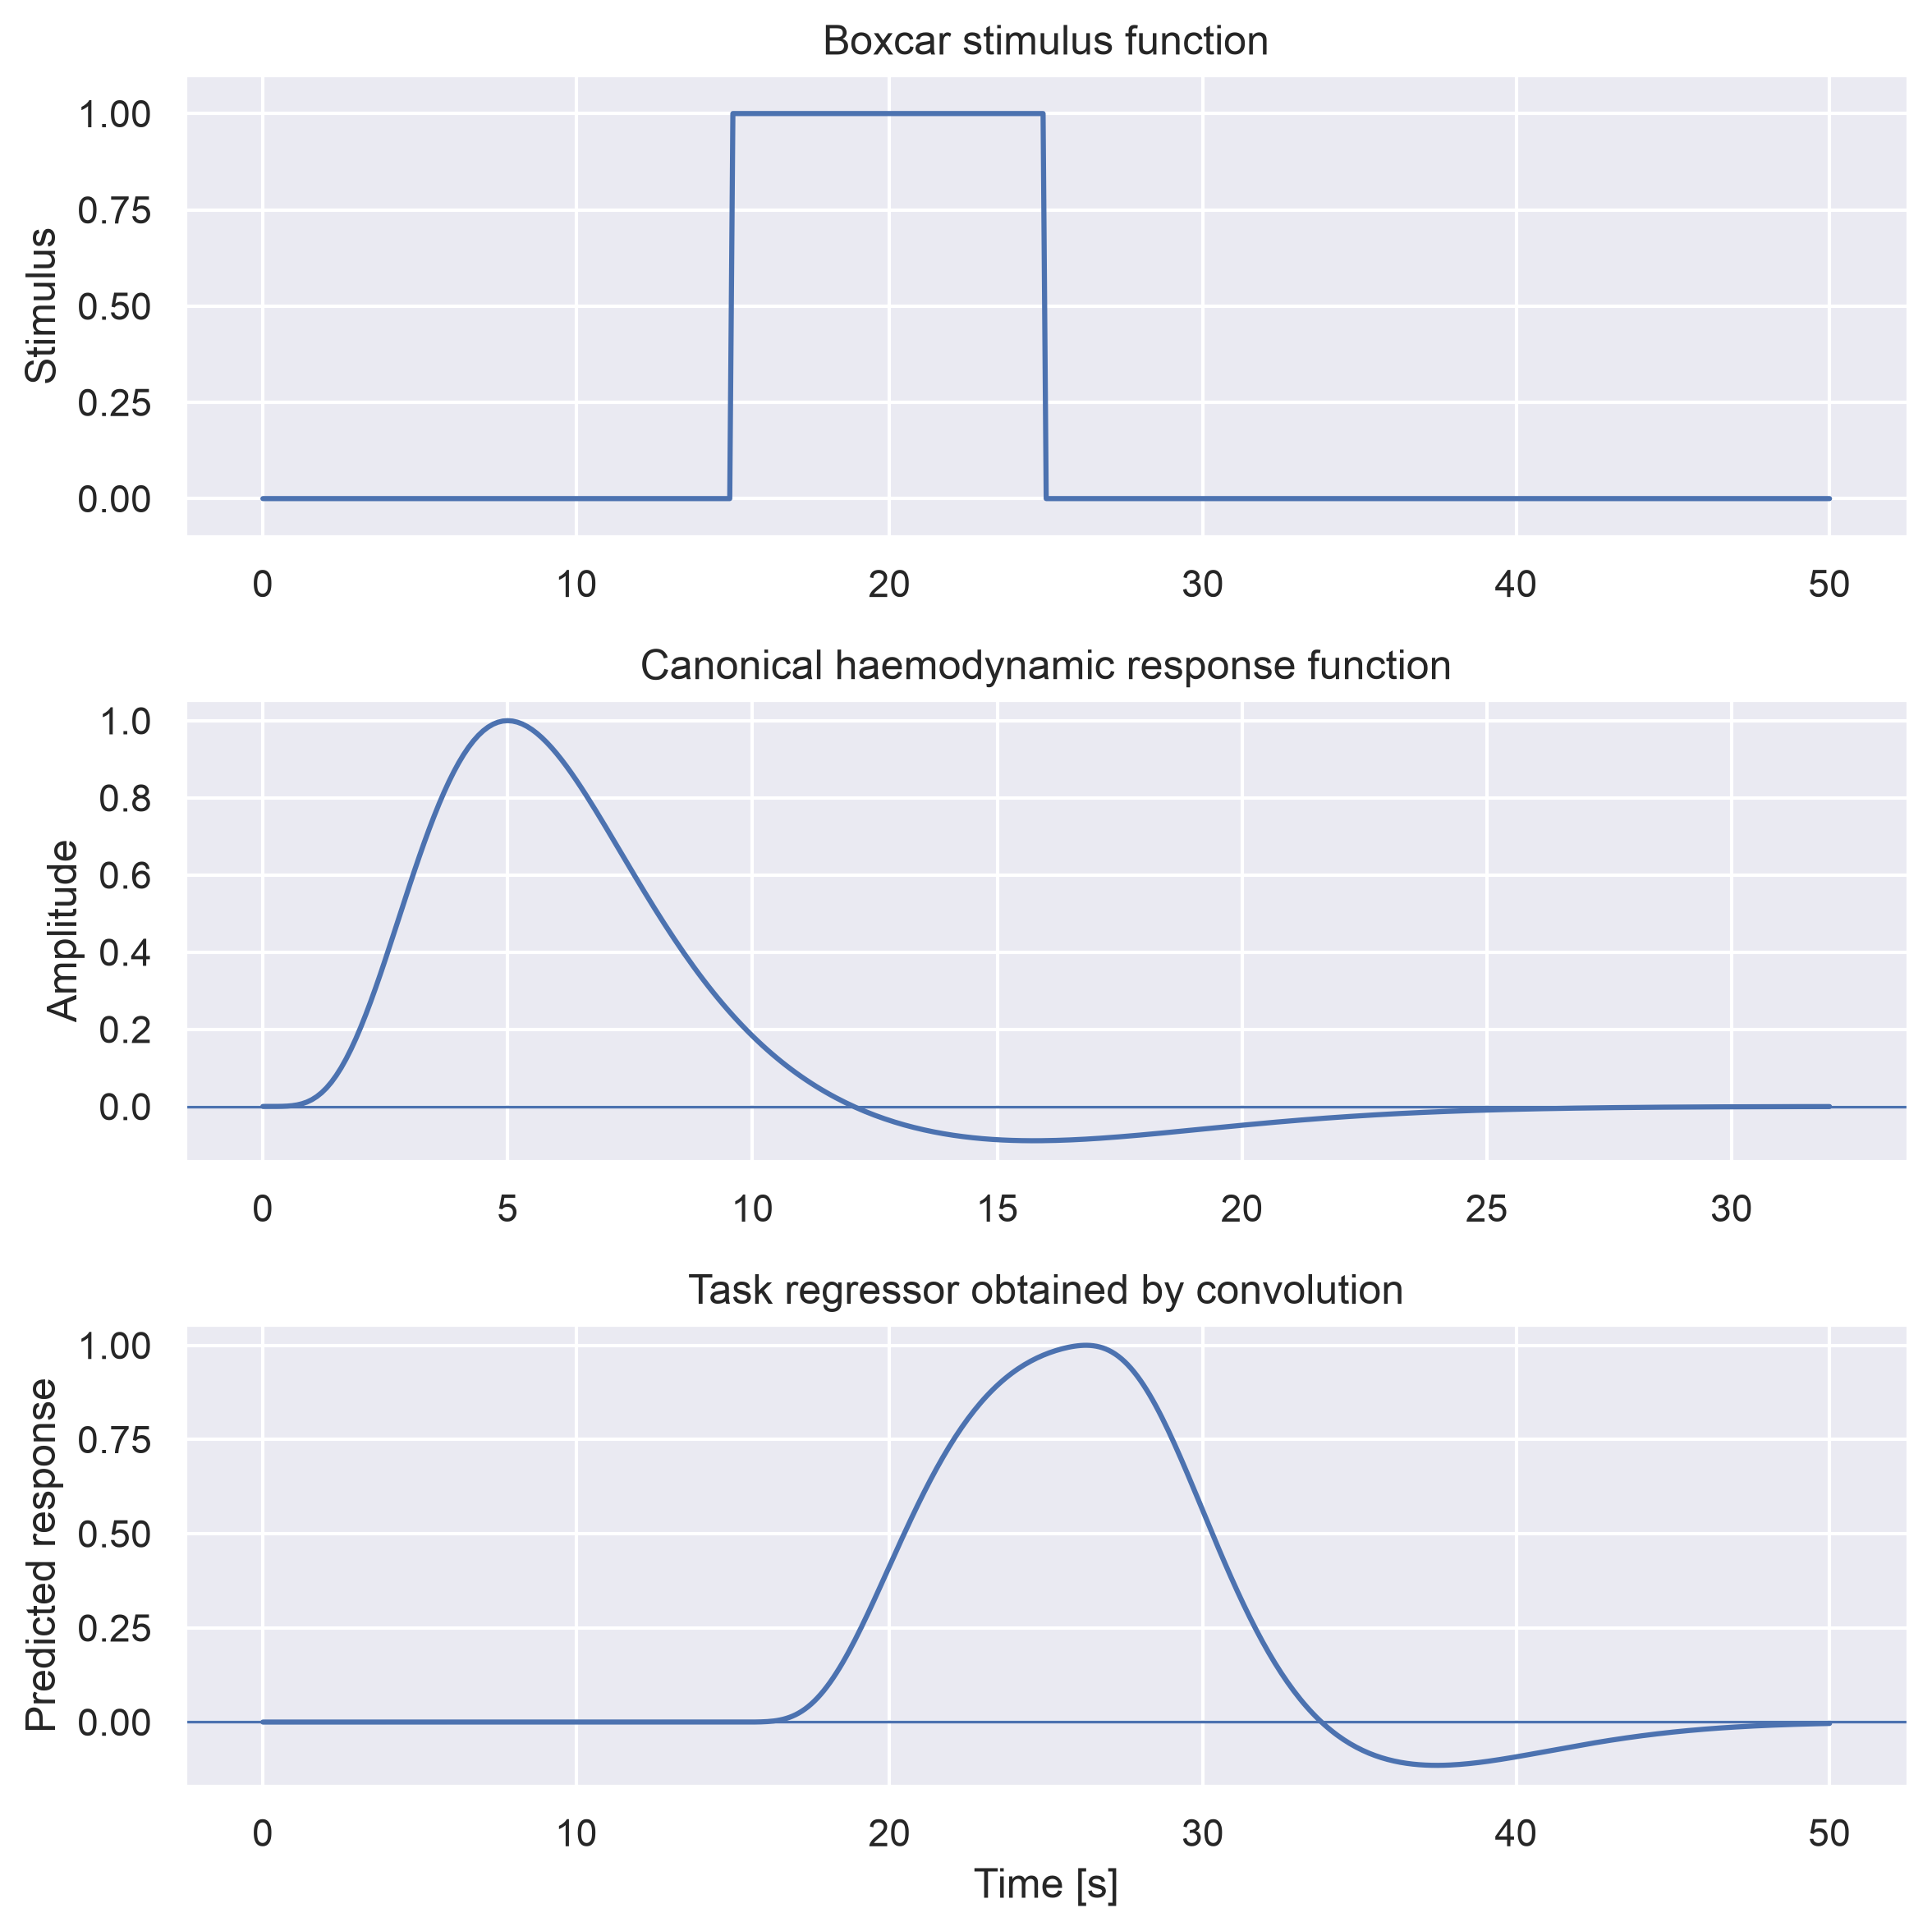
\includegraphics[scale=0.5]{fig/example_hrf_boxcar_convolution.png}
    \caption{Example showing a stimulus function active over the interval $[15.0\,\mathrm{s}, 25.0\,\mathrm{s}]$, the canonical HRF, and their convolution.}
    \label{fig:hrf-boxcar-convolution}
\end{figure}

\subsection{Nuisance regressors}

The remaining part of the design matrix contains nuisance regressors. These regressors model structured sources of variability that are not considered part of the task-related response. They do not reproduce all forms of noise exactly. Instead, they provide explanatory variables whose fitted contributions can be removed from the observed signal.

The nuisance part of the design matrix may be written as

\begin{equation}
    \mathbf{X}_{\mathrm{nuis}} =
    \begin{bmatrix}
        \mathbf{X}_{\mathrm{intercept}} & \mathbf{X}_{\mathrm{drift}} & \mathbf{X}_{\mathrm{motion}} & \mathbf{X}_{\mathrm{physio}} & \mathbf{X}_{\mathrm{data}}
    \end{bmatrix}.
    \label{eq:nuisance-design}
\end{equation}

Not all of the inner matrices must be present in every analysis. Their inclusion depends on the available measurements and the selected denoising procedure. Data-derived nuisance regressors based on PCA, presented in Equation~\eqref{eq:nuisance-design} as $\mathbf{X}_{\mathrm{data}}$, will be introduced in Section~\ref{section:pca-regressors}.

\subsubsection{Motion and physiological regressors}

Motion regressors are commonly included in fMRI models to account for signal changes associated with participant movement. A standard set contains three translation parameters and three rotation parameters estimated during motion correction \cite{motion-correction}. The raw dataset analyzed in this thesis does not include precomputed motion parameters, hence explicit motion regressors were not included in the design matrix.

Physiological regressors may be constructed from respiratory and cardiac recordings acquired during scanning. These regressors can account for signal changes related to breathing, cardiac pulsation, and variations in heart rate or respiratory volume. The dataset does not contain such measurements. Therefore, physiological regressors based on external recordings are not included.

The absence of explicit motion or physiological regressors does not imply that the corresponding effects are absent from the data. Some of this variability may remain in the residuals or may later be captured by data-derived nuisance regressors.

\subsubsection{Drift regressors}

Drift regressors are included to model low-frequency changes in the fMRI signal. Such changes may appear because of scanner instabilities, slow participant movement, thermal effects, or other slow-varying processes \cite{drift-others}.

Low-frequency drift can be represented using polynomial functions, splines, or Discrete Cosine Transform (DCT) basis functions. In this thesis, a DCT-II basis is considered. DCT regressors provide a controlled representation of low-frequency variation without overfitting the drift regressors to the actual desired BOLD signal.

Let $n$ denote the number of time points in a run. A DCT-II basis function can be written as \cite{dct}

\begin{equation}
    d_k(i) = \cos \left(\frac{\pi k(2i+1)}{2n}\right), \qquad i=0,\ldots,n-1, \qquad k=0,\ldots,K.
\end{equation}

Note that the constant component corresponding to $k=0$ produces an intercept column.

The number of DCT regressors should depend on the duration of the run and the selected high-pass cutoff \cite{spm-filter}. If $T$ denotes the run duration and $\tau_c$ denotes the cutoff period, an approximate rule is

\begin{equation}
    K = \left\lfloor\frac{2T}{\tau_c}\right\rfloor.
\end{equation}

Only the low-frequency basis functions below the selected cutoff are included. The cutoff must be chosen carefully because including too many DCT regressors may remove slow task-related variation together with signal drift. For the analyzed dataset, each run lasts approximately 300 seconds, but the number of DCT regressors cannot be determined from the run duration alone. It also requires an explicit choice of the cutoff period $\tau_c$, which in this thesis is the default value provided by SPM \cite{spm-filter} $\tau_c = 128 \, \mathrm{s}$.

Including the DCT basis in the design matrix is equivalent to modeling the selected low-frequency trends jointly with the task-related regressors. Their fitted contribution can then be treated as part of the nuisance signal and removed according to Equation~\eqref{eq:glm-denoised-signal}.

\newpage

\section{Standard GLM denoising}
\label{section:standard-glm}

The first denoising procedure considered in this thesis is referred to as standard GLM. It combines the task-related regressors described in Subsection~\ref{section:task-regressors} with the intercept and DCT drift regressors introduced above. The regression coefficients are estimated using the FGLS procedure with the run-specific AR(1) temporal covariance model described in Section~\ref{section:ar-noise-model}.

After model fitting, the contribution associated with the nuisance regressors is subtracted from the observed signal according to Equation~\eqref{eq:glm-denoised-signal}. The resulting procedure serves as the baseline method for comparison with the PCA-assisted GLM and ICA-based denoising introduced later.

The PCA-assisted GLM introduced in the following section extends this model by adding data-derived nuisance regressors obtained using PCA.

\section{PCA-derived nuisance regressors}
\label{section:pca-regressors}

The method used in this thesis is inspired by GLMdenoise, introduced in \cite{glm-denoise}. It extends GLM-based denoising by deriving additional nuisance regressors directly from the fMRI data. The method utilizes the multiple-run structure of the experiment and an inner leave-one-run-out cross-validation procedure to construct the noise pool, described in Subsection~\ref{section:selection-noise}, and select the number of nuisance regressors, described in Subsection~\ref{section:cv-pca-number}. This inner cross-validation is part of the PCA-assisted GLM fitting procedure and should be distinguished from the outer cross-validation used for final model evaluation, which is described in Chapter~\ref{chapter:evaluation}.

The procedure follows the main structure of GLMdenoise, with two modifications. First, the drift component is represented using the DCT regressors introduced earlier rather than the polynomial regressors used in the original method. Second, Ordinary Least Squares is replaced by the Feasible Generalized Least Squares (FGLS) procedure developed in the previous sections.

\subsection{Selection of the noise pool}
\label{section:selection-noise}

An initial model is fitted without PCA-derived nuisance regressors. Within the inner cross-validation procedure, one run is left out and the model is fitted to all remaining runs, as described in Section~\ref{section:caveats}. When the PCA-assisted GLM is subsequently evaluated within the outer cross-validation framework, further described in Section~\ref{section:outer-cv-evaluation}, this inner procedure is performed using only the runs belonging to the outer training set. 

The training design matrices contain the task-related and drift regressors. The task-related coefficients are shared across runs, while drift and other run-specific nuisance coefficients are estimated separately for each run. When the training runs are combined, the task-related parts of the design matrices are stacked vertically, while run-specific nuisance regressors are placed in separate columns.


For a single run, the covariance structure was derived in Equation~\eqref{eq:estimated-ar1-covariance}. Therefore, for the combined training data, the covariance matrix has the block-diagonal form:

\begin{equation}
    \widehat{\mathbf{V}}^{(-j)} =
    \operatorname{blockdiag}
    \left(\widehat{\mathbf{V}}_1, \ldots, \widehat{\mathbf{V}}_{j-1}, \widehat{\mathbf{V}}_{j+1}, \ldots, \widehat{\mathbf{V}}_R\right),
\end{equation}

where $j$ denotes the left-out run and the index $-j$ denotes quantities constructed using all runs except run $j$. $R$ is the total number of runs.

For example, if $R = 3$ and the second run is left out, then

\begin{equation}
    \widehat{\mathbf{V}}^{(-2)}
    =
    \operatorname{blockdiag}
    \left(
        \widehat{\mathbf{V}}_1,
        \widehat{\mathbf{V}}_3
    \right)
    =
    \begin{bmatrix}
        \widehat{\mathbf{V}}_1 & \mathbf{0} \\
        \mathbf{0} & \widehat{\mathbf{V}}_3
    \end{bmatrix}.
\end{equation}


After fitting the model, the estimated task-related coefficients are used to predict the task-related signal in the left-out run:

\begin{equation}
    \widehat{\mathbf{Y}}_{\mathrm{task},j}^{(-j)} = \mathbf{X}_{\mathrm{task},j} \widehat{\mathbf{B}}_{\mathrm{task}}^{(-j)}.
    \label{eq:pca-cv-task-prediction}
\end{equation}

The procedure is repeated until every run has been left out once. The predictions and measured signals are then concatenated across runs. Before calculating the coefficient of determination, the drift regressors are projected out from both the measured and predicted time series.

For voxel $v$, the coefficient of determination is defined as \cite[Equation 3.]{coefficient-determination}

\begin{equation}
    R^2_{v} = 1 - \frac{SS_{\text{resid}}}{SS_{\text{tot}}} 
    = 1 - \frac{\sum_{\tau = 1}^t \left(y_{\tau v} - \widehat{y}_{\tau v}\right)^2}{\sum_{\tau = 1}^t \left(y_{\tau v} - \overline{y}_v \right)^2},
    \label{eq:r2-calculation}
\end{equation}

where the index $\tau$ denotes a given time point in the voxel time series, $y_{\tau v}$ is the observed signal, $\widehat{y}_{\tau v}$ is the predicted signal, and $\overline{y}_v$ is the mean observed signal for voxel $v$.

This coefficient is not to be mistaken with the Pearson correlation coefficient squared $r^2$, which cannot have negative values. For the coefficient of determination $R^2$ a negative value coefficient results from sum of squared residuals being greater than total sum of squares, which indicates that the task-related model predicts the unseen data less accurately than a model that predicts only the mean signal \cite{coefficient-determination}.

After all folds of the inner cross-validation have been completed, the left-out predictions and the corresponding observed time series are concatenated across folds. The coefficient of determination is then computed using the same definition as in Equation~\eqref{eq:r2-calculation}, but using these concatenated predictions. This cross-validated coefficient of determination for voxel $v$ is denoted by $R^2_{\mathrm{CV},v}$. Voxels are included in the noise pool if they satisfy

\begin{equation}
    R^2_{\mathrm{CV},v} < 0,
\end{equation}

as described in \cite{glm-denoise}. This reduces the risk of including task-related voxels. 

In the original GLMdenoise procedure, an additional mean-intensity threshold is used to prevent voxels outside the brain from entering the noise pool \cite{glm-denoise}. In the present implementation, the analyzed voxel set is already restricted using an explicit brain mask, which is described in more detail in Section~\ref{section:evaluation-r2}. Therefore, this additional intensity criterion is not applied.

\subsection{Construction of the noise-pool matrices}

For each run $r$, the time series of the selected voxels are collected in a matrix

\begin{equation}
    \mathbf{Y}_{\mathrm{noise},r} \in \mathbb{R}^{t \times M},
\end{equation}

where $M$ is the number of voxels in the noise pool. Each column contains the time series of one voxel.

\newpage
Before PCA is performed, the drift contribution is projected out, similarly to Equation~\eqref{eq:ols-residuals-hat}. This is done, so that the PCA does not include the parts, that the DCT drift regressors explain. Let $\mathbf{P}_r$ denote the matrix containing the DCT drift regressors (including intercept) for run $r$. Its projection matrix and the projected-out noise-pool matrix are

\begin{equation}
    \mathbf{H}_{P_r} = \mathbf{P}_r \left(\mathbf{P}_r^T\mathbf{P}_r\right)^{-1}\mathbf{P}_r^T, 
    \qquad 
    \widetilde{\mathbf{Y}}_{\mathrm{noise},r} = \left(\mathbf{I} - \mathbf{H}_{P_r}\right) \mathbf{Y}_{\mathrm{noise},r}.
\end{equation}

Additionally, reflecting the procedure in \cite{glm-denoise}, after out-projecting the drift and baseline offsets contributions, each time series, i.e., each column $\mathbf{y}_j$ in $\widetilde{\mathbf{Y}}_{\mathrm{noise}} = \begin{bmatrix}\mathbf{y}_1 & \ldots &  \mathbf{y}_M\end{bmatrix}$, 
is normalized to unit length, such that

\begin{equation}
    \widehat{\mathbf{y}}_j = \frac{\mathbf{y}_j}{||\mathbf{y}_j||_2}.
\end{equation}

Denote the out-projected and normalized matrix as $\mathbf{Z}_r = \begin{bmatrix}\widehat{\mathbf{y}}_1 & \ldots &  \widehat{\mathbf{y}}_M\end{bmatrix}$. PCA is then applied separately to the prepared noise-pool matrix of each run. The details of Principal Component Analysis are described in Subsection~\ref{section:pca}. Using singular value decomposition,

\begin{equation}
    \mathbf{Z}_r = \mathbf{U}_r \mathbf{L}_r \mathbf{A}_r^T.
\end{equation}

The columns of $\mathbf{U}_r$ are orthogonal and provide the principal components. The first columns correspond to the directions associated with the largest amounts of variance~\cite{pca}. They are treated as candidate temporal nuisance regressors for run $r$. For a candidate number $k$, the PCA-derived nuisance-regressor matrix contains all columns up to, and including, column $k$. Such matrix will have the form of $\mathbf{U}_r^{(k)}$.

\subsection{Inner cross-validation of PCA-derived regressors}
\label{section:cv-pca-number}

For maximum candidate number $k_{\max}$ of principal components, each $k \in \left\{0,1,\ldots,k_{\max}\right\}$ requires a separate design matrix:

\begin{equation}
    \mathbf{X}_r^{(k)} =
    \begin{bmatrix}
        \mathbf{X}_{\mathrm{task},r} & \mathbf{P}_r & \mathbf{U}_r^{(k)}
    \end{bmatrix}.
\end{equation}

Inner leave-one-run-out cross-validation is then performed for each value of $k$. Its purpose is model selection rather than final performance evaluation. In each iteration:

\begin{enumerate}
    \item The run $j$ is left out.
    \item The model is fitted to all runs $r\neq j$ using FGLS.
    \item The task-related coefficients are estimated from the training runs.
    \item The task-related signal in the left-out run $j$ is predicted using its task design matrix and the task-related coefficients estimated from the training runs, according to Equation~\eqref{eq:pca-cv-task-prediction}.
\end{enumerate}

After all folds have been completed, the voxelwise cross-validated coefficient of determination is calculated for each candidate number of components. Only voxels for which the $R^2 > 0$ are chosen for candidates evaluation.

\newpage
For each value of $k$, the median performance is 

\begin{equation}
    m(k) = \operatorname*{median}_{v\in\mathcal{V}_{\mathrm{eval}}} R^2_{\mathrm{CV},v}(k),
\end{equation}

where the common evaluation set is defined as 

\begin{equation}
    \mathcal{V}_{\mathrm{eval}}
    = \left\{v : \max_{0\leq k\leq k_{\max}} R^2_{\mathrm{CV},v}(k) > 0\right\}.
\end{equation}

The improvement relative to the model without PCA-derived nuisance regressors is then defined as

\begin{equation}
    \Delta(k) = m(k)-m(0), \qquad \Delta_{\max} = \max_{0\leq k\leq k_{\max}} \Delta(k).
\end{equation}

Reflecting the procedure of \cite{glm-denoise}, the selected number of nuisance regressors $k^\ast$ is the smallest value satisfying $\Delta(k) \geq 0.95 \Delta_{\max}$. This ensures selection of a model whose improvement is within $5\%$ of the maximum observed improvement. It avoids adding components that provide little additional predictive benefit and which can lead to overfitting.

Finally, after $k^\ast$ has been selected, the model containing $k^\ast$ PCA-derived regressors is refitted using all runs available to the internal procedure. During outer cross-validation, these correspond to the outer training runs. The fitted PCA contribution is then treated as part of the nuisance signal and can be removed according to the denoising procedure defined earlier.

The final evaluation of both the standard GLM introduced in Section~\ref{section:standard-glm} and the PCA-assisted GLM described in Section~\ref{section:pca-regressors} is performed using the common outer cross-validation framework described in Chapter~\ref{chapter:evaluation}.


\subsection{Principal Component Analysis}
\label{section:pca}

Principal Component Analysis is used here to derive a low-dimensional set of nuisance regressors from the time series of the noise-pool voxels. Its main purpose is to reduce dimensionality while preserving as much of the variance in the original data as possible.

PCA represents the data using principal components, which are mutually orthogonal linear combinations of the original variables. The first principal component explains the largest possible amount of variance in the data. Each subsequent component explains the largest possible remaining variance while being orthogonal to all preceding components. The derivations and examples presented in this subsection follow the approach in \cite{pca}.

Let $\mathbf{X}$ be a data matrix and $\boldsymbol{\Sigma}$ its sample covariance matrix:

\begin{equation}
    \mathbf{X} \in \mathbb{R}^{n\times p}, \qquad \boldsymbol{\Sigma} = \frac{1}{n-1}\mathbf{X}^T\mathbf{X}
\end{equation}

The first loading vector $\boldsymbol{\alpha}_1$ maximizes:

\begin{equation}
    \operatorname{Var} \left[ \mathbf{X}\boldsymbol{\alpha_1} \right] 
    = \boldsymbol{\alpha}_1^T \boldsymbol{\Sigma}\boldsymbol{\alpha}_1 
    \quad \text{subject to} \quad 
    \boldsymbol{\alpha}_1^T \boldsymbol{\alpha}_1 = 1.
\end{equation}

The second loading vector 
$\boldsymbol{\alpha}_2$ maximizes $\operatorname{Var}\left[\mathbf{X}\boldsymbol{\alpha}_2\right]$ subject to being uncorrelated with $\mathbf{X}\boldsymbol{\alpha}_1$, meaning $\operatorname{Cov}\left[\mathbf{X}\boldsymbol{\alpha}_1, \mathbf{X}\boldsymbol{\alpha}_2\right] = 0$. For $k$-th loading vector this procedure is repeated, maximizing $\operatorname{Var}\left[\mathbf{X}\boldsymbol{\alpha}_k\right]$, subject to being uncorrelated with $\mathbf{X}\boldsymbol{\alpha}_1, \ldots, \mathbf{X}\boldsymbol{\alpha}_{k-1}$. The loading vectors $\boldsymbol{\alpha}_1, \ldots \boldsymbol{\alpha}_k$ are the eigenvectors of the covariance matrix $\boldsymbol{\Sigma}$.

\newpage
In this thesis, PCA is computed using singular value decomposition \cite[Section 3.5]{pca}. Let the rank of $\mathbf{X}$ be $r$. Its reduced SVD is

\begin{equation}
    \mathbf{X} = \mathbf{U} \mathbf{L} \mathbf{A}^T,
    \label{eq:svd}
\end{equation}

where

\begin{equation}
    \mathbf{U} \in \mathbb{R}^{n\times r}, \qquad \mathbf{A} \in \mathbb{R}^{p\times r}, \qquad \mathbf{L} \in \mathbb{R}^{r\times r}.
\end{equation}

The columns of $\mathbf{U}$ and $\mathbf{A}$ are orthonormal \cite[Section 3.5]{pca}, while $\mathbf{L}$ is a diagonal matrix:

\begin{equation}
    \mathbf{U}^T\mathbf{U} = \mathbf{I}_r, \qquad \mathbf{A}^T\mathbf{A} = \mathbf{I}_r, \qquad \mathbf{L} = \operatorname{diag} \left(\ell_1, \ell_2, \ldots \ell_r\right).
\end{equation}

From Equation~\eqref{eq:svd},

\begin{equation}
    \begin{aligned}
        \mathbf{X}^T\mathbf{X} 
        &= \mathbf{A} \mathbf{L}^T \mathbf{U}^T  \, \mathbf{U} \mathbf{L} \mathbf{A}^T  \\
        &= \mathbf{A} \mathbf{L}^T \mathbf{I} \mathbf{L} \mathbf{A}^T \\
        &= \mathbf{A} \mathbf{L} \mathbf{L} \mathbf{A}^T \\
        &= \mathbf{A} \mathbf{L}^2 \mathbf{A}^T. 
    \end{aligned}
\end{equation}

Thus, the columns of $\mathbf{A}$ are eigenvectors of $\mathbf{X}^T\mathbf{X}$ and of the sample covariance matrix $\boldsymbol{\Sigma}$. The corresponding covariance eigenvalues are

\begin{equation}
    \lambda_j = \frac{\ell_j^2}{n-1}.
\end{equation}

The principal-component score matrix is

\begin{equation}
    \mathbf{Z} = \mathbf{X}\mathbf{A} = \mathbf{U}\mathbf{L}.
\end{equation}

Therefore, the columns of $\mathbf{U}\mathbf{L}$ contain the principal-component scores, while the columns of $\mathbf{U}$ contain normalized versions of these scores.

In the present application, the observations are time points and the variables are noise-pool voxels. The leading temporal principal components are used as candidate nuisance regressors.


\newpage
\chapter{Independent Component Analysis}
\label{chapter:ica}

Independent Component Analysis (ICA) is closely related to blind source separation \cite{blind-source-separation}, which aims to recover source signals from observed mixtures without prior knowledge of the mixing or filtering processes.

ICA can be presented with a commonly used example: the \textit{cocktail-party problem} \mbox{\cite[Section 7.1]{ica}}. Suppose that three people are speaking simultaneously in a room and the sound they are emitting is recorded using three microphones in three different locations. Each microphone records a different mixture of the three speech signals. The observed signals can be represented as weighted sums of the signals emitted by the speakers:

\begin{equation}
    \begin{aligned}
        x_1(t) &= a_{11}s_1(t) + a_{12}s_2(t) + a_{13}s_3(t), \\
        x_2(t) &= a_{21}s_1(t) + a_{22}s_2(t) + a_{23}s_3(t), \\
        x_3(t) &= a_{31}s_1(t) + a_{32}s_2(t) + a_{33}s_3(t),
    \end{aligned}
\end{equation}

where

\begin{itemize}
    \item $x_i(t)$ is the signal recorded by the $i$-th microphone,
    \item $s_j(t)$ is the signal emitted by the $j$-th speaker,
    \item $a_{ij}$ is a parameter which depends on the distance between the $i$-th microphone and the  $j$-th speaker.
\end{itemize}

If the coefficients $a_{ij}$ were known, the original signals could be recovered by solving the corresponding linear system. The problem is that neither the coefficients $a_{ij}$ nor the original source signals $s_j(t)$ are known. Both the separation and the source is therefore referred to as \textit{blind}.

In ICA terminology, a source is an unknown hidden signal represented by an independent component \cite{ica}. The goal is to recover these sources using only their observed \textit{mixtures}, meaning the linear or non-linear combination of unknown latent variables, using an unknown mixing system.

The classical square ICA mixing model can be written as

\begin{equation}
    \mathbf{X} = \mathbf{A}\mathbf{S},
    \label{eq:basic-ica}
\end{equation}

where

\begin{equation}
    \mathbf{X} \in \mathbb{R}^{n\times m},
    \qquad
    \mathbf{A} \in \mathbb{R}^{n\times n}, 
    \qquad
    \mathbf{S} \in \mathbb{R}^{n\times m}.
    \label{eq:basic-ica-dimensions}
\end{equation}

In \eqref{eq:basic-ica-dimensions}, $n$ is the number of observed mixtures, while $m$ is the number of observations. The rows of $\mathbf{S}$ contain the unknown source signals, while $\mathbf{A}$ is the unknown mixing matrix. The application of this model to fMRI data will be discussed in Section~\ref{section:pica}.

In the cocktail-party example, these matrices have the following representation:

\begin{equation}
    \mathbf{X} = \begin{bmatrix}x_1(t) \\ x_2(t) \\ x_3(t)\end{bmatrix}
    , \qquad
    \mathbf{A} = 
    \begin{bmatrix}
    a_{11} & a_{12} & a_{13} \\ 
    a_{21} & a_{22} & a_{23} \\ 
    a_{31} & a_{32} & a_{33} \\ 
    \end{bmatrix}
    , \qquad
    \mathbf{S} = \begin{bmatrix}s_1(t) \\ s_2(t) \\ s_3(t)\end{bmatrix}
\end{equation}

\section{Assumptions of the ICA model}

The principal assumption of ICA is the independence of the source components. Let

\begin{equation}
    \mathbf{s} = \left(s_1, \ldots, s_n\right)^T
\end{equation}

denote a random vector of source variables. Their independence implies that their joint probability density factorizes as

\begin{equation}
    p(s_1, \ldots, s_n) = \prod_{i=1}^{n}p_i(s_i).
\end{equation}

The second important assumption is that the independent components are non-Gaussian. More precisely, no independent components, or at most one independent component, may have a Gaussian distribution \cite[p. 163]{ica}.

The reason for this restriction can be illustrated with an example from \cite[Section~7.5]{ica}. Using two independent standard Gaussian variables, meaning with zero mean and unit variance, let

\begin{equation}
    \mathbf{s} = \begin{bmatrix}
        s_1 \\
        s_2
    \end{bmatrix}
    \sim \mathcal{N} \left(\mathbf{0}, \mathbf{I}\right).
\end{equation}

Their joint density is

\begin{equation}
    p_{\mathbf{s}}(\mathbf{s}) = \frac{1}{2\pi} \exp \left(-\frac{\|\mathbf{s}\|_2^2}{2}\right).
\end{equation}

Suppose that the mixing matrix $\mathbf{A}$ is orthogonal, so that $\mathbf{A}^{-1} = \mathbf{A}^T$. For $\mathbf{x} = \mathbf{A}\mathbf{s}$, the density of $\mathbf{x}$ is

\begin{equation}
    p_{\mathbf{x}}(\mathbf{x}) = p_{\mathbf{s}} \left(\mathbf{A}^{-1}\mathbf{x}\right) \left|\det\left(\mathbf{A}^{-1}\right)\right|.
\end{equation}

Since an orthogonal transformation preserves the Euclidean norm,

\begin{equation}
    \left\|\mathbf{A}^{-1}\mathbf{x} \right\|_2^2
    = \left\|\mathbf{A}^T\mathbf{x}\right\|_2^2
    = (\mathbf{A}^T\mathbf{x})^T(\mathbf{A}^T\mathbf{x})
    = \mathbf{x}^T\mathbf{A}\mathbf{A}^T\mathbf{x}
    = \|\mathbf{x}\|_2^2,
\end{equation}

and

\begin{equation}
    |\det(\mathbf{A})|=1.
\end{equation}

Therefore,

\begin{equation}
    p_{\mathbf{x}}(\mathbf{x}) = \frac{1}{2\pi} \exp \left(-\frac{\|\mathbf{x}\|_2^2}{2}\right).
\end{equation}

Thus, an orthogonal transformation of a standardized Gaussian vector produces the same probability distribution. This means that the original directions cannot be identified from Gaussianity alone and non-Gaussianity is necessary for identifying the independent components.

For the classical square ICA model in Equation~\eqref{eq:basic-ica}, the number of independent components is equal to the number of observed mixtures. If $\mathbf{A}$ is nonsingular, the source matrix can be recovered using an unmixing matrix

\begin{equation}
    \mathbf{W} = \mathbf{A}^{-1},
\end{equation}

so that

\begin{equation}
    \mathbf{S} = \mathbf{W}\mathbf{X}.
\end{equation}

For ICA, the scale of an independent component cannot be determined uniquely because a scaling factor can be transferred between a source and the corresponding column of the mixing matrix. Moreover, if the source variance is fixed, a sign ambiguity still remains. Additionally, permutations of the components and the corresponding columns of the mixing matrix do not change the observed data.

These ambiguities concern the representation of a fixed number of independent components. For fMRI data, however, another problem must be addressed first: finding the number of unknown components before estimating them.

\section{Dimensionality reduction and model order selection}
\label{section:pica}

ICA can be analyzed both in the context of spatial or temporal independent components~\cite{spatial-temporal-ica}. The spatial ICA focuses on finding spatially independent maps, i.e., maps that connect the data from multiple voxels into an independent response. An example of such a map can be a joint response of left and right hemispheres to a flashing light stimuli. The temporal ICA focuses on finding temporally independent time courses. An example of such a time course could be a cyclical response seen after each block of flashing lights.

Generally, the neuroimaging literature focuses on spatial ICA, because $V >> T$, meaning the number of voxel samples is generally greater than the number of time points. The temporal ICA under a small number of time points is statistically and computationally more complex, while the sparse nature of the typical spatial activation response is said to be working well with spatial ICA \cite{spatial-temporal-ica}. Hence, for this thesis the spatial ICA was chosen.

The classical ICA model described in Equation~\eqref{eq:basic-ica} assumes a square mixing matrix. For spatial ICA applied to fMRI data, the observed data matrix can be written as

\begin{equation}
    \mathbf{X} \in \mathbb{R}^{t \times v},
\end{equation}

where $t$ denotes the number of time points and $v$ denotes the number of voxels. Therefore, the rows correspond to observed brain data for all voxels at a given time point, while the columns contain the time series measured at individual voxels.


\newpage
Under the classical square ICA formulation~\eqref{eq:basic-ica}, the model would take the form

\begin{equation}
    \mathbf{X} = \mathbf{A}\mathbf{S},
    \qquad \mathbf{A} \in \mathbb{R}^{t\times t},
    \qquad \mathbf{S} \in \mathbb{R}^{t\times v}.
\end{equation}

The number of independent components would therefore be equal to the number of time points. This classical ICA assumption about the shape of the matrices does not allow the signal to be restricted to a lower-dimensional subspace \cite{pica}.

A second problem is that the classical model does not contain an explicit noise term. The data are assumed to be completely represented by the estimated sources and the mixing matrix. In noisy fMRI data, this may lead to overfitting, since variability caused by observational noise may be represented as additional components rather than as residual noise \cite{pica}. Dimensionality reduction is also commonly used before ICA to reduce noise and decrease this overfitting risk \cite[Section 13.2]{ica}.

To address these problems, the authors of \cite{pica} introduced a Probabilistic Independent Component Analysis (PICA) model for fMRI. The classical model is extended to

\begin{equation}
    \mathbf{X} = \mathbf{A}\mathbf{S} + \mathbf{E},
    \label{eq:pica-model}
\end{equation}

where

\begin{equation}
    \mathbf{X} \in \mathbb{R}^{t\times v},
    \qquad \mathbf{A} \in \mathbb{R}^{t\times q},
    \qquad \mathbf{S} \in \mathbb{R}^{q\times v},
    \qquad \mathbf{E} \in \mathbb{R}^{t\times v},
    \label{eq:pica-dimensions}
\end{equation}

and $q<t$ denotes the unknown number of latent source processes. The columns of $\mathbf{A}$ contain the time series associated with the components, while the rows of $\mathbf{S}$ contain their spatial maps. In spatial ICA, statistical independence is imposed on these spatial source maps.

For an individual voxel $i$, the model can equivalently be written as

\begin{equation}
    \mathbf{x}_i = \mathbf{A}\mathbf{s}_i + \boldsymbol{\eta}_i,
    \label{eq:pica-not-whitened}
\end{equation}

where

\begin{equation}
    \mathbf{x}_i \in \mathbb{R}^{t}, \qquad 
    \mathbf{s}_i \in \mathbb{R}^{q}, \qquad 
    \mathbf{A} \in \mathbb{R}^{t\times t}, \qquad
    \boldsymbol{\eta}_i \in \mathbb{R}^t,
\end{equation}

and $\boldsymbol{\eta}_i$ denotes additive Gaussian observational noise. Following \cite{pica}, its distribution can be represented as

\begin{equation}
    \boldsymbol{\eta}_i \sim \mathcal{N}\left(\mathbf{0}, \sigma^2\boldsymbol{\Sigma}_i\right), 
    \qquad \mathbb{E} \left[\boldsymbol{\eta}_i\right] = \mathbf{0},
    \qquad \operatorname{Cov} (\boldsymbol{\eta}_i) = \sigma^2\boldsymbol{\Sigma}_i
\end{equation}

The covariance structure of the noise is unknown and must therefore be estimated from the data. The authors of \cite{pica} propose constraining the temporal noise covariance to an autoregressive form and re-estimating it from model residuals, following the approach of \cite{woolrich-temporal-autocorrelation}. The estimation of an autoregressive temporal covariance model from residuals was introduced earlier in Section~\ref{section:ar-noise-model} as $\mathbf{V}$ in Equation~\eqref{eq:estimated-ar1-covariance}.

Before dimensionality reduction, the data can be temporally prewhitened with respect to this covariance structure. The following derivations mirror the derivations from~\cite{pica}. Since the estimated covariance matrix is utilized, in this thesis a single covariance matrix $\mathbf{V}$ is used, instead of a covariance matrix $\boldsymbol{\Sigma}_i$ for an individual voxel, hence the index $i$ is dropped. This covariance matrix is symmetric and positive definite.

\newpage
Let

\begin{equation}
    \boldsymbol{\Sigma} = \mathbf{L}\mathbf{L}^T
\end{equation}

be a decomposition of $\boldsymbol{\Sigma}$ into an $\mathbf{L}$ lower-triangular matrix and its transpose $\mathbf{L}^T$, i.e., Cholesky decomposition \cite{cholesky}. Left multiplication of \eqref{eq:pica-not-whitened} by $\mathbf{L}^{-1}$ gives

\begin{equation}
    \begin{aligned}
        \overline{\mathbf{x}}_i
        &= \mathbf{L}^{-1}\mathbf{x}_i \\
        &= \mathbf{L}^{-1}\mathbf{A}\mathbf{s}_i + \mathbf{L}^{-1}\boldsymbol{\eta}_i.
    \end{aligned}
    \label{eq:pica-temporal-whitening}
\end{equation}

The transformed noise $\overline{\boldsymbol{\eta}}_i$ has covariance

\begin{equation}
    \begin{aligned}
        \operatorname{Cov} \left(\overline{\boldsymbol{\eta}}_i\right)
        &= \mathbf{L}^{-1} \sigma^2\boldsymbol{\Sigma}_i \left(\mathbf{L}^{-1}\right)^T \\
        &= \sigma^2 \mathbf{L}^{-1} \mathbf{L} \mathbf{L}^T \left(\mathbf{L}^{-1}\right)^T \\
        &= \sigma^2\mathbf{I}.
    \end{aligned}
\end{equation}

This is prewhitening with respect to the temporal covariance structure of the regression errors, which is called \textit{temporal prewhitening}. It is closely related to the prewhitening introduced earlier for the GLM in Definition~\ref{def:prewhitening} and should not be confused with the PCA-based whitening used later during ICA estimation in Section~\ref{section:ica-whitening}.

After temporal prewhitening, the problem of determining the number of source signals can be considered under an isotropic noise model, meaning a model with a covariance proportional to the identity matrix $\operatorname{Cov}(\overline{\boldsymbol{\eta}}) = \sigma^2 \mathbf{I}$. From this point onward, the bars are omitted for notational simplicity, and $\mathbf{X}$ denotes the temporally prewhitened data. Assume that the sources have zero mean and unit covariance,

\begin{equation}
    \mathbb{E}[\mathbf{s}_i] = \mathbf{0}, \qquad \operatorname{Cov}(\mathbf{s}_i) = \mathbf{I}_q.
\end{equation}

The covariance matrix of the observations is then

\begin{align}
    \mathbf{C}
    &= \operatorname{Cov}(\mathbf{x}_i) \\
    &= \mathbf{A} \operatorname{Cov}(\mathbf{s}_i) \mathbf{A}^T + \sigma^2\mathbf{I} \\
    &= \mathbf{A}\mathbf{A}^T + \sigma^2\mathbf{I}.
    \label{eq:pica-observation-covariance}
\end{align}

Since $\mathbf{A}\in\mathbb{R}^{t\times q}$ is assumed to have full column rank:

\begin{equation}
    \operatorname{rank}(\mathbf{A}) = \operatorname{rank} \left( \mathbf{A}\mathbf{A}^T \right) = q.
\end{equation}

The eigendecomposition of the signal contribution can therefore be written as

\begin{equation}
    \mathbf{A}\mathbf{A}^T = \mathbf{U} \boldsymbol{\Gamma} \mathbf{U}^T,
\end{equation}

where $\mathbf{U}$ is an orthogonal matrix, and $\boldsymbol{\Gamma}$ is a diagonal matrix

\begin{equation}
    \boldsymbol{\Gamma} = \operatorname{diag} \left(\gamma_1,\ldots,\gamma_q, 0,\ldots,0\right),
\end{equation}

with

\begin{equation}
    \gamma_1 \geq \gamma_2 \geq \cdots \geq \gamma_q > 0.
\end{equation}

\newpage
Using the eigendecomposition of matrix $\mathbf{C}$

\begin{equation}
    \mathbf{C} = \mathbf{U} \boldsymbol{\Lambda} \mathbf{U}^T,
\end{equation}

and Equation~\eqref{eq:pica-observation-covariance}, the $\mathbf{C}$ can be written as

\begin{equation}
\begin{aligned}
    \mathbf{C}
    &= \mathbf{U} \boldsymbol{\Gamma} \mathbf{U}^T + \sigma^2\mathbf{I} \\
    &= \mathbf{U} \left(\boldsymbol{\Gamma} + \sigma^2\mathbf{I} \right) \mathbf{U}^T \\
    &= \mathbf{U} \boldsymbol{\Lambda} \mathbf{U}^T
\end{aligned}
\end{equation}

Therefore the eigenvalues of $\mathbf{C}$ are the eigenvalues of $\boldsymbol{\Lambda}$, and consequently the eigenvalues of $\boldsymbol{\Gamma} + \sigma^2 \mathbf{I}$, which take the form

\begin{equation}
    \lambda_j =
    \begin{cases}
        \gamma_j+\sigma^2, & j=1,\ldots,q, \\
        \sigma^2, & j=q+1,\ldots,t.
    \end{cases}
\end{equation}

Hence,

\begin{equation}
    \lambda_1 \geq \cdots \geq \lambda_q > \lambda_{q+1} = \lambda_{q+2} = \cdots = \lambda_t = \sigma^2.
\end{equation}

The first $q$ eigenvectors span the latent source subspace, while the remaining $(t-q)$ eigenvectors span the Gaussian noise subspace. In this setting, model order selection becomes the problem of estimating the value of $q$ that separates these two subspaces.

This distinction is important because an inappropriate value of $q$ can affect the ICA decomposition:

\begin{itemize}
    \item if $q$ is too small, some structured source processes may be removed during dimensionality reduction;
    \item if $q$ is too large, directions dominated by Gaussian observational noise may be included in the ICA decomposition, increasing the risk of overfitting.
\end{itemize}

Unfortunately, the covariance matrix $\mathbf{C}$ is unknown. For centered data, it is estimated from the observed fMRI matrix as

\begin{equation}
    \widehat{\mathbf{C}} = \frac{1}{v} \mathbf{X}\mathbf{X}^T.
    \label{eq:pica-covariance-matrix}
\end{equation}

Even if the true noise is isotropic and Gaussian, the eigenvalues $\widehat{\lambda}_{q+1}, \cdots, \widehat{\lambda}_t$, later called \textit{minor} eigenvalues of the covariance matrix, will not all be exactly equal to $\sigma^2$. The observed noise eigenspectrum instead fluctuates around the true value. Consequently, simply searching for an exact equality in the observed minor eigenspectrum is not sufficient for correct model order selection \cite{pica}.

In \cite{pica}, the authors formulate this step using Probabilistic Principal Component Analysis (PPCA). For the purpose of model order estimation, the source variables are temporarily assumed to be Gaussian. This assumption is used only to estimate the dimensionality of the source subspace and is dropped, once the independent components are identified. The final ICA decomposition still searches for non-Gaussian independent spatial sources.

\newpage
Performing the eigendecomposition of the sample covariance matrix

\begin{equation}
    \widehat{\mathbf{C}} = \widehat{\mathbf{U}} \widehat{\boldsymbol{\Lambda}} \widehat{\mathbf{U}}^T,
    \label{eq:eig-covariance}
\end{equation}

provides the eigenspectrum $\widehat{\boldsymbol{\Lambda}} = \operatorname{diag}\left(\widehat{\lambda}_1, \ldots, \widehat{\lambda}_t\right)$ of $\widehat{\mathbf{C}}$. For a fixed candidate value $q$, the maximum-likelihood estimate of the isotropic noise variance is obtained by averaging the eigenvalues associated with the minor subspace spanned by $(t - q)$ eigenvectors \cite{pica}:

\begin{equation}
    \widehat{\sigma}_{\mathrm{ML}}^2(q) = \frac{1}{t-q} \sum_{j=q+1}^{t} \widehat{\lambda}_j.
\end{equation}

This maximum-likelihood estimator is then calculated for each candidate value $q$.

Under the Gaussian noise model, the sample covariance matrix follows a Wishart distribution. This allows the expected finite-sample distribution of its eigenvalues to be characterized and compared with the observed minor eigenspectrum \cite{pica}.

Let $\mathbf{G}$ be a $p \times n$ matrix whose columns are independent realizations of a $p$-variate normal distribution with zero mean $\mathbf{g}_i \sim \mathcal{N}(\mathbf{0}, \mathbf{V})$. The probability distribution of the matrix $\mathbf{G}\mathbf{G}^T$ has a Wishart distribution $W_p(\mathbf{V}, n)$ with scale matrix $\mathbf{V}$ and $n$ degrees of freedom. In the high-dimensional limit, where both $p$ and $n$ increase while their ratio $c = \frac{p}{n}$ remains fixed, the empirical distribution of the eigenvalues of the corresponding sample covariance matrix converges to the Marchenko-Pastur distribution \cite{pica}. Its density is

\begin{equation}
    g_c(\nu) = \frac{\sqrt{(\nu - b_-)(b_+ - \nu)}}{2\pi c\nu},
    \qquad
    b_\pm = (1 \pm \sqrt{c})^2,
    \qquad \nu \in [b_-, b_+].
\end{equation}

The cumulative distribution function corresponding to $g_c$ can then be used to obtain the expected quantiles of the noise eigenspectrum. These quantiles describe the eigenvalue spread that is expected purely as a consequence of finite sampling \cite{pica}.

Following \cite{pica}, the predicted Gaussian-noise eigenspectrum is then used to adjust the observed eigenspectrum before evaluating the approximate Bayesian model evidence described in \cite[Equation 10]{pica}. The model evidence is calculated for every candidate model order $q$. The selected model order is

\begin{equation}
    \widehat{q} = \arg\max_q p(\mathbf{X}\mid q).
\end{equation}

Once the model order $\widehat{q}$ has been selected, the first $\widehat{q}$ eigenvectors of $\widehat{\mathbf{C}}$, i.e., the first $\widehat{q}$ columns of $\widehat{\mathbf{U}}$, define the estimated PPCA source subspace. Let

\begin{equation}
    \widehat{\mathbf{U}}_{\widehat{q}} \in \mathbb{R}^{t\times\widehat{q}}
\end{equation}

contain these eigenvectors. The observed data can then be projected onto this subspace:

\begin{equation}
    \mathbf{X}_{\widehat{q}} = \widehat{\mathbf{U}}_{\widehat{q}}^T \mathbf{X},
    \qquad \mathbf{X}_{\widehat{q}} \in \mathbb{R}^{\widehat{q}\times v}.
    \label{eq:pica-dimensionality-reduction}
\end{equation}

The dimensionality has been reduced from the original $t$ temporal mixtures to $\widehat{q}$ mixtures. The reduced representation contains the estimated structured source subspace, while the remaining directions are treated as Gaussian observational noise. The reduced dimensionality model with the extension of noise, introduced in Equation~\eqref{eq:pica-model}, can therefore be expressed as

\begin{equation}
    \mathbf{X}_{\widehat{q}} 
    = \widehat{\mathbf{U}}_{\widehat{q}}^T \mathbf{X}
    = \widehat{\mathbf{U}}_{\widehat{q}}^T \mathbf{A}\mathbf{S} + \widehat{\mathbf{U}}_{\widehat{q}}^T\mathbf{E}.
\end{equation}

\newpage
Probabilistic ICA is used here to motivate the noisy model and to estimate the dimensionality of the structured source subspace. After selecting $\widehat{q}$, the subsequent source estimation is performed using the classical noise-free ICA approximation within this retained subspace

\begin{equation}
    \mathbf{X}_{\widehat{q}} \approx \widehat{\mathbf{U}}_{\widehat{q}}^T \mathbf{A}\mathbf{S}.
    \label{eq:noise-free-ica-approx}
\end{equation}

Thus, residual observational noise may still be present in the retained subspace, but it is no longer modeled explicitly in the subsequent FastICA estimation.

\section{Whitening}
\label{section:ica-whitening}

After dimensionality reduction, ICA is performed within the estimated $\widehat{q}$-dimensional source subspace. Before estimating the independent components, the reduced data are whitened. This is a second and conceptually different transformation from the temporal prewhitening introduced in the previous section in Equation~\eqref{eq:pica-temporal-whitening}, since temporal prewhitening acts along the time dimension and is used to account for autocorrelation in the observational noise. Conversely, the whitening conducted in this section will be guided by the same principles as in Section~\ref{section:gls-prewhitening}. The whitening presented in this section acts upon the reduced ICA space and removes correlations between the mixture variables.

Let the centered data in the reduced space be $\mathbf{X}_{\widehat{q}}$ and let a whitening matrix $\mathbf{K}$ transform it into

\begin{equation}
    \mathbf{Z} = \mathbf{K}\mathbf{X}_{\widehat{q}},
    \label{eq:ica-whitening}
\end{equation}

where 

\begin{equation}
    \qquad \mathbf{Z} \in \mathbb{R}^{\widehat{q} \times v}
    , \qquad \mathbf{K} \in \mathbb{R}^{\widehat{q} \times \widehat{q}}
    , \qquad \mathbf{X}_{\widehat{q}} \in \mathbb{R}^{\widehat{q} \times v},
\end{equation}

such that the sample covariance matrix of the whitened observations is

\begin{equation}
    \operatorname{Cov}(\mathbf{Z}) = \frac{1}{v}\mathbf{Z}\mathbf{Z}^T = \mathbf{I}_{\widehat{q}}.
    \label{eq:whitened-covariance-pica}
\end{equation}

Suppose that $\mathbf{D}$ is an arbitrary orthogonal matrix and

\begin{equation}
    \mathbf{Z}^{\ast} = \mathbf{D}\mathbf{Z}.
\end{equation}

Then

\begin{equation}
    \begin{aligned}
        \operatorname{Cov}\left(\mathbf{Z}^{\ast}\right) &= \mathbf{D} \operatorname{Cov}(\mathbf{Z}) \mathbf{D}^T \\
        &= \mathbf{D} \mathbf{I}_{\widehat{q}} \mathbf{D}^T \\
        &= \mathbf{I}_{\widehat{q}}.
    \end{aligned}
\end{equation}

Therefore, infinitely many possible rotations $\mathbf{D}$ preserve the whitened covariance structure. However, whitening alone cannot determine which of these rotations produces statistically independent components.

\newpage
Under the classical noise-free ICA approximation adopted after model-order selection in Equation~\eqref{eq:noise-free-ica-approx}, define the mixing matrix in the reduced space as

\begin{equation}
    \mathbf{A}_{\widehat{q}} := \widehat{\mathbf{U}}_{\widehat{q}}^T \mathbf{A},
\end{equation}

where $\mathbf{A}_{\widehat{q}} \in \mathbb{R}^{\widehat{q} \times \widehat{q}}$. The reduced model can therefore be written as

\begin{equation}
    \mathbf{X}_{\widehat{q}} = \mathbf{A}_{\widehat{q}}\mathbf{S}.
    \label{eq:noise-free-ica}
\end{equation}

Assume that the source components are centered and scaled to unit variance, so that

\begin{equation}
    \operatorname{Cov}(\mathbf{S}) = \frac{1}{v}\mathbf{S}\mathbf{S}^T = \mathbf{I}_{\widehat{q}}.
\end{equation}

Considering the corresponding noise-free ICA representation within the retained subspace, represented in Equation~\ref{eq:noise-free-ica}, its whitened representation is:

\begin{equation}
    \mathbf{Z} = \mathbf{K}\mathbf{X}_{\widehat{q}} = \mathbf{K}\mathbf{A}_{\widehat{q}}\mathbf{S} =: \widetilde{\mathbf{A}}\mathbf{S}
    \label{eq:whitened-data}
\end{equation}

where $\widetilde{\mathbf{A}} \in \mathbb{R}^{\widehat{q} \times \widehat{q}}$. For the square whitened model,

\begin{equation}
    \begin{aligned}
        \operatorname{Cov}\left(\mathbf{Z}\right) = \mathbf{I}_{\widehat{q}}
        &= \frac{1}{v} \mathbf{Z}\mathbf{Z}^T \\
        &= \widetilde{\mathbf{A}} \left(\frac{1}{v} \mathbf{S}\mathbf{S}^T \right) \widetilde{\mathbf{A}}^T \\
        &= \widetilde{\mathbf{A}} \mathbf{I}_{\widehat{q}} \widetilde{\mathbf{A}}^T \\
        &= \widetilde{\mathbf{A}} \widetilde{\mathbf{A}}^T. 
    \end{aligned}
\end{equation}

Thus, $\widetilde{\mathbf{A}}$ is orthogonal. Instead of estimating an arbitrary mixing matrix, ICA can therefore search over orthogonal transformations of the whitened data.

To estimate the whitening matrix $\mathbf{K}$, the eigenvalue decomposition of the covariance matrix is used, similarly to the whitening done in Section~\ref{section:gls-prewhitening}. Let 

\begin{equation}
    \widehat{\mathbf{C}}_{\widehat{q}} = \operatorname{Cov}\left(\mathbf{X}_{\widehat{q}}\right)
\end{equation}

be the covariance matrix of the retained representation within the selected subspace. This covariance matrix can be simplified, following Equation~\eqref{eq:pica-covariance-matrix} and the eigendecomposition of the sample covariance matrix presented in Equation~\eqref{eq:eig-covariance}

\begin{equation}
    \begin{aligned}
        \widehat{\mathbf{C}}_{\widehat{q}}
        &= \frac{1}{v} \mathbf{X}_{\widehat{q}} \mathbf{X}_{\widehat{q}}^T \\
        &= \frac{1}{v} \widehat{\mathbf{U}}_{\widehat{q}}^T \mathbf{X} \mathbf{X}^T \widehat{\mathbf{U}}_{\widehat{q}} \\
        &= \widehat{\mathbf{U}}_{\widehat{q}}^T \widehat{\mathbf{C}} \widehat{\mathbf{U}}_{\widehat{q}} \\
        &= \widehat{\mathbf{U}}_{\widehat{q}}^T \widehat{\mathbf{U}} \widehat{\boldsymbol{\Lambda}} \widehat{\mathbf{U}}^T \widehat{\mathbf{U}}_{\widehat{q}}
    \end{aligned}
    \label{eq:subspace-covariance-matrix}
\end{equation}

We can present the orthogonal matrix $\widehat{\mathbf{U}}$ as 

\begin{equation}
    \widehat{\mathbf{U}} = \begin{bmatrix}\widehat{\mathbf{U}}_{\widehat{q}} & \widehat{\mathbf{U}}_\perp \end{bmatrix},
\end{equation}

where

\begin{equation}
    \widehat{\mathbf{U}} \in \mathbb{R}^{t \times t}, \qquad
    \widehat{\mathbf{U}}_{\widehat{q}} \in \mathbb{R}^{t \times \widehat{q}}, \qquad
    \widehat{\mathbf{U}}_\perp \in \mathbb{R}^{t \times \left(t - \widehat{q}\right)}.
\end{equation}

Because all columns of $\widehat{\mathbf{U}}$ are orthonormal

\begin{equation}
    \widehat{\mathbf{U}}_{\widehat{q}}^T \widehat{\mathbf{U}}_{\widehat{q}} = \mathbf{I}_{\widehat{q}},
\end{equation}

and 

\begin{equation}
    \widehat{\mathbf{U}}_{\widehat{q}}^T \widehat{\mathbf{U}}_\perp = \mathbf{0}.
\end{equation}

Therefore

\begin{equation}
    \widehat{\mathbf{U}}_{\widehat{q}}^T \widehat{\mathbf{U}} 
    = \widehat{\mathbf{U}}_{\widehat{q}}^T \begin{bmatrix}\widehat{\mathbf{U}}_{\widehat{q}} & \widehat{\mathbf{U}}_\perp \end{bmatrix}
    = \begin{bmatrix}\widehat{\mathbf{U}}_{\widehat{q}}^T\widehat{\mathbf{U}}_{\widehat{q}} & \widehat{\mathbf{U}}_{\widehat{q}}^T\widehat{\mathbf{U}}_\perp \end{bmatrix}
    = \begin{bmatrix} \mathbf{I}_{\widehat{q}} & \mathbf{0} \end{bmatrix},
\end{equation}

and analogously

\begin{equation}
    \widehat{\mathbf{U}}^T \widehat{\mathbf{U}}_{\widehat{q}}
    = \begin{bmatrix} \mathbf{I}_{\widehat{q}} \\ \mathbf{0} \end{bmatrix}.
\end{equation}

Furthermore, partitioning the eigenvalue matrix $\widehat{\boldsymbol{\Lambda}}$

\begin{equation}
    \widehat{\boldsymbol{\Lambda}} = 
    \begin{bmatrix}
        \widehat{\boldsymbol{\Lambda}}_{\widehat{q}} & \mathbf{0} \\
        \mathbf{0} & \widehat{\boldsymbol{\Lambda}}_\perp     
    \end{bmatrix}
\end{equation}

The derivation of the covariance matrix in \eqref{eq:subspace-covariance-matrix} continues 

\begin{equation}
    \begin{aligned}
        \widehat{\mathbf{C}}_{\widehat{q}}
        &= \widehat{\mathbf{U}}_{\widehat{q}}^T \widehat{\mathbf{U}} \widehat{\boldsymbol{\Lambda}} \widehat{\mathbf{U}}^T \widehat{\mathbf{U}}_{\widehat{q}} \\
        &= 
            \begin{bmatrix} 
                \mathbf{I}_{\widehat{q}} & \mathbf{0} 
            \end{bmatrix} 
            \begin{bmatrix}
                \widehat{\boldsymbol{\Lambda}}_{\widehat{q}} & \mathbf{0} \\
                \mathbf{0} & \widehat{\boldsymbol{\Lambda}}_\perp     
            \end{bmatrix}
            \begin{bmatrix} 
                \mathbf{I}_{\widehat{q}} \\ \mathbf{0} 
            \end{bmatrix} \\
        &= \widehat{\boldsymbol{\Lambda}}_{\widehat{q}}.
    \end{aligned}
\end{equation}

Following the whitening presented in \cite[Equation 7.20]{ica}, the whitening matrix is therefore 

\begin{equation}
    \mathbf{K} = \widehat{\boldsymbol{\Lambda}}_{\widehat{q}}^{-1/2}.
\end{equation}

The whitened data in Equation~\eqref{eq:ica-whitening} are therefore

\begin{equation}
    \mathbf{Z} =  \mathbf{K}\mathbf{X}_{\widehat{q}}
    = \widehat{\boldsymbol{\Lambda}}_{\widehat{q}}^{-1/2} \widehat{\mathbf{U}}_{\widehat{q}}^T \mathbf{X},
\end{equation}

and the resulting covariance is

\begin{equation}
    \begin{aligned}
        \operatorname{Cov}(\mathbf{Z}) 
        &= \mathbf{K} \operatorname{Cov}(\mathbf{X_{\widehat{q}}}) \mathbf{K}^T \\
        &= \widehat{\boldsymbol{\Lambda}}_{\widehat{q}}^{-1/2} \widehat{\boldsymbol{\Lambda}}_{\widehat{q}} \left(\widehat{\boldsymbol{\Lambda}}_{\widehat{q}}^{-1/2} \right)^T \\
        &= \widehat{\boldsymbol{\Lambda}}_{\widehat{q}}^{-1/2} \widehat{\boldsymbol{\Lambda}}_{\widehat{q}} \widehat{\boldsymbol{\Lambda}}_{\widehat{q}}^{-1/2} \\
        &= \mathbf{I}_{\widehat{q}},
    \end{aligned}
\end{equation}

proving the whitening assertion in Equation~\eqref{eq:whitened-covariance-pica}.


\section{Estimation of independent components with FastICA}

As shown in the previous sections, after dimensionality reduction and whitening, the ICA model can be written as

\begin{equation}
    \mathbf{Z} = \widetilde{\mathbf{A}}\mathbf{S},
\end{equation}

where $\widetilde{\mathbf{A}} \in \mathbb{R}^{\widehat{q}\times \widehat{q}}$ is orthogonal. Therefore,

\begin{equation}
    \mathbf{S} = \widetilde{\mathbf{A}}^{-1} \mathbf{Z} = \widetilde{\mathbf{A}}^T \mathbf{Z}.
\end{equation}

The remaining ICA problem therefore consists of estimating the appropriate orthogonal transformation of the whitened observations. Following the notation of \cite{pica}, let

\begin{equation}
    \mathbf{Q} := \widetilde{\mathbf{A}}^T.
    \label{eq:q-orthogonal}
\end{equation}

The estimated independent components can then be written as

\begin{equation}
    \widehat{\mathbf{S}} = \mathbf{Q}\mathbf{Z}.
    \label{eq:estimated-ics}
\end{equation}

To obtain the estimation of independent components presented in \cite[Section 8.4]{ica}, consider a single whitened observation $\mathbf{z} \in \mathbb{R}^{\widehat{q}}$ for a fixed component direction $\mathbf{q} \in \mathbb{R}^{\widehat{q}}$, corresponding to one row of $\mathbf{Q}$. The corresponding scalar projection is 

\begin{equation}
    y = \mathbf{q}^T \mathbf{z}.
    \label{eq:scalar-projection}
\end{equation}

The main idea of the ICA component estimation is to search for directions for which the projected data are as non-Gaussian as possible. One measure of non-Gaussianity is negentropy \cite[Equation 8.22]{ica}:

\begin{equation}
    J(y) = H(y_{\mathrm{gauss}}) - H(y),
\end{equation}

where $y_{\mathrm{gauss}}$ is a Gaussian random variable with the same variance as $y$, and

\begin{equation}
    H(y) = -\int p_y(\eta) \log p_y(\eta)\,\mathrm{d}\eta
\end{equation}

is the differential entropy of $y$.

A Gaussian random variable has the largest entropy among random variables with the same variance \cite[Section 5.3.2]{ica}. Therefore,

\begin{equation}
    J(y)\geq 0,
\end{equation}

with equality if $y$ is Gaussian.

For whitened data, the search for one independent component can therefore be written as

\begin{equation}
    \mathbf{q}^{\ast} = \arg\max_{\|\mathbf{q}\|_2^2=1} J \left(\mathbf{q}^T\mathbf{z}\right).
\end{equation}

\newpage
From the variance of the scalar projection presented in Equation~\eqref{eq:scalar-projection}, the constraint of unit-norm needs to be imposed, since

\begin{equation}
    \begin{aligned}
        \operatorname{Var}
        \left( \mathbf{q}^T\mathbf{z} \right)
        &= \mathbf{q}^T \operatorname{Cov}(\mathbf{z}) \mathbf{q} \\
        &= \mathbf{q}^T\mathbf{q} \\
        &= \|\mathbf{q}\|_2^2.
    \end{aligned}
\end{equation}

Thus, setting $\|\mathbf{q}\|_2^2=1$ fixes the variance of the extracted component and prevents arbitrary changes in scale.

The problem of negentropy, is that it requires knowledge or estimation of the probability density function. This is computationally complex, so an algorithm called \textit{FastICA} was developed, which uses an approximation based on a suitable function $G(y)$ \mbox{\cite[Equation 8.25]{ica}:}

\begin{equation}
    J(y) \propto \left( \mathbb{E}[G(y)] - \mathbb{E}[G(\nu)]\right)^2.
\end{equation}

The expected values are present, following their definition:

\begin{equation}
    H(y) = -\int p_y(\eta) \log p_y(\eta)\,\mathrm{d}\eta = - \mathbb{E} \left[ \log p_y(y) \right],
\end{equation}

while $\nu$ denotes a standardized Gaussian random variable. Squaring captures the magnitude of the difference and preserves non-negative values in the negentropy. 

The authors of \cite{ica} state that the approximation function $G(y)$ should be nonquadratic and have its values not grow too rapidly as $|y|$ increases. Several possible representations of the $G(y)$ function are provided in \cite{ica}. This thesis uses a good general-purpose function~\cite{ica}:

\begin{equation}
    G(y) = \ln (\cosh y), \qquad g(y) = G'(y) = \tanh y, \qquad g'(y) = G''(y) = 1 - \tanh^2 y
\end{equation}

FastICA uses an approximate Newton fixed-point iteration. For one component, the update is \cite[Equation 8.43]{ica}

\begin{equation}
    \mathbf{q}^{+} = \mathbb{E} \left[ \mathbf{z} g \left( \mathbf{q}^T\mathbf{z} \right) \right]
    - \mathbb{E} \left[g' \left( \mathbf{q}^T\mathbf{z} \right)\right] \mathbf{q},
\end{equation}

followed by normalization:

\begin{equation}
    \mathbf{q}_{\mathrm{new}} = \frac{\mathbf{q}^{+}}{\|\mathbf{q}^{+}\|_2}.
\end{equation}

The procedure is repeated until the direction of $\mathbf{q}$ converges. The convergence criterion~is 

\begin{equation}
    \mathbf{q}_{\mathrm{new}} = \pm \mathbf{q}
\end{equation}

Since $\mathbf{q}$ and $-\mathbf{q}$ represent the same component up to its sign ($(-\mathbf{q})^T\mathbf{z} = -\mathbf{q}^T\mathbf{z}$), the convergence criterion is insensitive to this sign ambiguity, as is ICA.

When several components are estimated simultaneously, the corresponding vectors are collected in the unmixing matrix in the whitened space, denoted by $\mathbf{Q}$. The vectors must additionally be decorrelated so that multiple iterations do not converge to the same component. 

\newpage
In the symmetric FastICA algorithm, this is performed using symmetric orthogonalization:

\begin{equation}
    \mathbf{Q} \gets \left( \mathbf{Q}\mathbf{Q}^T \right)^{-1/2}\mathbf{Q}.
\end{equation}

Although the authors of the book \cite{ica} do not explicitly state the convergence criterion, a natural stopping point would be when 

\begin{equation}
    \mathbf{q}_{\mathrm{new}} \approx \pm \mathbf{q}_{\mathrm{old}}.
\end{equation}

In practice this means that both the old and new vectors, representing the direction associated with a particular component of $\widehat{\mathbf{S}}$, have almost the same direction in relation to each other. Since these vectors are normalized, we can utilize the dot product to measure the cosine of the angle between them

\begin{equation}
    \mathbf{q}_{\mathrm{new}} \cdot \mathbf{q}_{\mathrm{old}} = \mathbf{q}_{\mathrm{new}}^T \mathbf{q}_{\mathrm{old}} = \cos \theta
\end{equation}

where $\theta$ is the angle between $\mathbf{q}_{\mathrm{new}}$ and $\mathbf{q}_{\mathrm{old}}$.

If the dot product is equal to $1$ (or $-1$), these vectors point in the same direction (opposite direction, respectively). The full convergence criterion can therefore be stated as

\begin{equation}
    \max_i \left(1 - |\mathbf{q}_i^T\mathbf{q}_{i,\mathrm{old}}| \right) < \varepsilon.
\end{equation}

If this convergence criterion is true, for small enough $\varepsilon$ it means, that the two vectors are nearly identical up to a sign.

The full algorithm in matrix notation, following the FastICA algorithm presented in \cite[Table 8.4]{ica}, can be seen in Table~\ref{alg:fastica}.

\begin{algorithm}[H]
\caption{Symmetric FastICA}
\label{alg:fastica}
\begin{algorithmic}[1]
    \Require Whitened observations $\mathbf{Z} \in \mathbb{R}^{\widehat{q}\times v}$
    \Require Nonlinear function $g$ and its derivative $g'$
    \Require Convergence tolerance $\varepsilon > 0$
    \Require $\mathbf{Q} = \mathbf{I}_{\widehat{q}}$

    \State Orthogonalize $\mathbf{Q}$

    \Repeat
        \State Store previous matrix:
        $$ \mathbf{Q}_{\mathrm{old}} \gets \mathbf{Q} $$

        \State Update all rows simultaneously:
        $$ 
        \mathbf{Q} \gets 
        \mathbb{E} \left[ g(\mathbf{Q}\mathbf{Z})\mathbf{Z}^T \right] 
        - \operatorname{diag} \left( \mathbb{E} \left[ g'(\mathbf{Q}\mathbf{Z}) \right] \right) \mathbf{Q}
        $$

        \State Apply symmetric orthogonalization:
        $$ \mathbf{Q} \gets (\mathbf{Q}\mathbf{Q}^T)^{-1/2}\mathbf{Q} $$

    \Until{$$ \max_i \left(1 - |\mathbf{q}_i^T\mathbf{q}_{i,\mathrm{old}}| \right) < \varepsilon $$}

    \State \Return
    $$ \widehat{\mathbf{S}} = \mathbf{Q} \mathbf{Z} $$
\end{algorithmic}
\end{algorithm}

Finally, after estimating the independent components in the whitened reduced space, the full unmixing matrix with respect to the temporally prewhitened observation space can be obtained by combining the dimensionality reduction, whitening, and ICA transformations. Using Equation~\eqref{eq:whitened-data} together with the projection defined in Equation~\eqref{eq:pica-dimensionality-reduction},

\begin{equation}
    \widehat{\mathbf{S}} = \mathbf{Q}\mathbf{Z} = \mathbf{Q}\mathbf{K}\mathbf{X}_{\widehat{q}} = \mathbf{Q}\mathbf{K}\widehat{\mathbf{U}}_{\widehat{q}}^T \mathbf{X}.
\end{equation}

Therefore, the full unmixing matrix mapping the prewhitened observations to the estimated independent components is

\begin{equation}
    \mathbf{W} = \mathbf{Q}\mathbf{K}\widehat{\mathbf{U}}_{\widehat{q}}^T,
\end{equation}

so that 

\begin{equation}
    \widehat{\mathbf{S}} = \mathbf{W}\mathbf{X}.
\end{equation}

The mixing matrix can be recovered by reversing the transformations applied before the estimation of the independent components. From the whitening transformation in Equation~\eqref{eq:ica-whitening},

\begin{equation}
    \mathbf{Z} = \mathbf{K}\mathbf{X}_{\widehat{q}},
\end{equation}

and therefore

\begin{equation}
    \mathbf{X}_{\widehat{q}} = \mathbf{K}^{-1}\mathbf{Z}.
\end{equation}

Furthermore, from the estimated ICs in Equation~\eqref{eq:estimated-ics}

\begin{equation}
    \widehat{\mathbf{S}} = \mathbf{Q}\mathbf{Z},
\end{equation}

and since $\mathbf{Q}$ was defined in Equation~\eqref{eq:q-orthogonal} as $\mathbf{Q} = \widetilde{\mathbf{A}}^T$, where $\widetilde{\mathbf{A}}$ is orthogonal, meaning $\mathbf{Q}$ is also orthogonal, its inverse is equal to its transpose. Hence,

\begin{equation}
    \mathbf{Z} = \mathbf{Q}^{-1}\widehat{\mathbf{S}} = \mathbf{Q}^T\widehat{\mathbf{S}}.
\end{equation}

Combining the two transformations gives 

\begin{equation}
    \mathbf{X}_{\widehat{q}} = \mathbf{K}^{-1}\mathbf{Q}^T\widehat{\mathbf{S}}.
\end{equation}

The representation in the original temporal space is obtained by mapping the reduced data back through the eigenvectors in Equation~\eqref{eq:pica-dimensionality-reduction}:

\begin{equation}
    \widehat{\mathbf{X}} = \widehat{\mathbf{U}}_{\widehat{q}}\mathbf{X}_{\widehat{q}}
    = \widehat{\mathbf{U}}_{\widehat{q}}\mathbf{K}^{-1}\mathbf{Q}^T\widehat{\mathbf{S}}.
\end{equation}

Comparing this expression with the ICA reconstruction in the retained subspace

\begin{equation}
    \widehat{\mathbf{X}} = \widehat{\mathbf{A}}\widehat{\mathbf{S}},
\end{equation}

gives the estimated mixing matrix

\begin{equation}
    \widehat{\mathbf{A}} = \widehat{\mathbf{U}}_{\widehat{q}}\mathbf{K}^{-1}\mathbf{Q}^T.
\end{equation}


\section{ICA-based denoising and component classification}
\label{section:ica-denoising}

The ICA decomposition described in the previous sections separates the observed data into statistically independent spatial components and their corresponding temporal courses. However, statistical independence alone does not determine whether a component represents variability related to the experimental task or variability that should be treated as nuisance. An additional classification procedure is therefore required before the ICA decomposition can be used for denoising.

The classification procedure used in this thesis is based on the ICA-based denoising method considered in \cite{glm-denoise}. In that approach, the temporal course associated with each independent component is compared with the task-related part of the experimental design. Components whose temporal courses exhibit sufficiently strong correspondence with the task are retained, whereas the remaining components are treated as nuisance and removed from the data.

To avoid ambiguity with the notation used for the GLM design matrix, let

\begin{equation}
    \mathbf{Y} \in \mathbb{R}^{t \times v}
\end{equation}

denote the fMRI data matrix, where $t$ is the number of time points and $v$ is the number of voxels. The spatial ICA model estimated for this run can be written as

\begin{equation}
    \mathbf{Y} = \widehat{\mathbf{A}} \widehat{\mathbf{S}},
\end{equation}

where

\begin{equation}
    \widehat{\mathbf{A}} \in \mathbb{R}^{t \times \widehat{q}},
    \qquad
    \widehat{\mathbf{S}} \in \mathbb{R}^{\widehat{q} \times v}.
\end{equation}

The $j$-th independent component is represented by the pair

\begin{equation}
    \left(\widehat{\mathbf{a}}_j, \, \widehat{\mathbf{s}}_j \right), \qquad
    \widehat{\mathbf{a}}_j \in \mathbb{R}^{t \times 1}, \qquad
    \widehat{\mathbf{s}}_j \in \mathbb{R}^{1 \times v}
\end{equation}

where $\widehat{\mathbf{a}}_j$ is the temporal course associated with the component and corresponds to the $j$-th column of the mixing matrix $\widehat{\mathbf{A}}$, and $\widehat{\mathbf{s}}_j$ is its spatial map and corresponds to the $j$-th row of the source matrix $\widehat{\mathbf{S}}$. Thus, the contribution of component $j$ to the observed data is the rank-one matrix

\begin{equation}
    \widehat{\mathbf{a}}_j \widehat{\mathbf{s}}_j.
\end{equation}

\subsection{Task-relatedness of the independent components}

Let

\begin{equation}
    \mathbf{X}_{\mathrm{task}} \in \mathbb{R}^{t \times p}
\end{equation}

denote the task-related part of the GLM design matrix, where in the considered experiment $p=8$, as described in Subsection~\ref{section:task-regressors}. For each ICA temporal course $\widehat{\mathbf{a}}_j$, its relationship with the experimental task is evaluated using the linear regression model

\begin{equation}
    \widehat{\mathbf{a}}_j = \mathbf{X}_{\mathrm{task}} \boldsymbol{\gamma}_j + \boldsymbol{\varepsilon}_j.
\end{equation}

\newpage
Assuming that $\mathbf{X}_{\mathrm{task}}$ has full column rank, similarly as in the Equation~\eqref{eq:ols-estimator}, the OLS estimator of the coefficient vector is

\begin{equation}
    \widehat{\boldsymbol{\gamma}}_j =
    \left(\mathbf{X}_{\mathrm{task}}^{T} \mathbf{X}_{\mathrm{task}} \right)^{-1}
    \mathbf{X}_{\mathrm{task}}^{T}
    \widehat{\mathbf{a}}_j.
\end{equation}

The fitted temporal course is therefore

\begin{equation}
    \widehat{\mathbf{a}}_{\mathrm{fit},j} = \mathbf{X}_{\mathrm{task}} \widehat{\boldsymbol{\gamma}}_j.
\end{equation}

The authors of \cite{glm-denoise} describe the classification criterion as the amount of variance in a component time course explained by the task-related regressors, but do not provide an explicit formula for this quantity. In this thesis, it is quantified using the coefficient of determination introduced in Equation~\eqref{eq:r2-calculation}, applied to the current component time course:

\begin{equation}
    R^2_{\mathrm{IC},j} = 1 - \frac{ \left| \widehat{\mathbf{a}}_j - \widehat{\mathbf{a}}_{\mathrm{fit}, j} \right|_2^2}{\left|| \widehat{\mathbf{a}}_j - \overline{a}_j \mathbf{1} \right||_2^2},
\end{equation}

where $\overline{a}_j$ is the mean of the temporal course. The notation $R^2_{\mathrm{IC}, j}$ is used to distinguish this quantity from the cross-validated coefficient of determination $R^2_{\mathrm{CV},v}$ used in Subsection~\ref{section:selection-noise} to evaluate voxelwise prediction accuracy.

A large value of $R^2_{\mathrm{IC},j}$ alone is not sufficient to classify the component as task-related, since some correspondence with the task design may occur by chance. Following \cite{glm-denoise}, the temporal order of each component course is therefore randomly permuted. Let

\begin{equation}
    \widehat{\mathbf{a}}_j^{(b)}, \qquad b=1,\ldots,B,
\end{equation}

denote the $b$-th randomly shuffled version of the temporal course, with $B=1000$. The same regression procedure is applied to every shuffled time course, producing

\begin{equation}
    R_{\mathrm{IC},j}^{2,(1)}, \ldots, R_{\mathrm{IC},j}^{2,(B)}.
\end{equation}

These values form an empirical reference distribution representing the task-related variance that can be obtained after the original temporal ordering of the component has been broken up. Its empirical mean and standard deviation are

\begin{equation}
    \mu_j = \frac{1}{B} \sum_{b=1}^{B} R_{\mathrm{IC},j}^{2,(b)}, \qquad
    \sigma_j =\sqrt{\frac{1}{B-1} \sum_{b=1}^{B} \left(R_{\mathrm{IC},j}^{2,(b)}-\mu_j \right)^2}.
\end{equation}

For convenience, the classification rule from \cite{glm-denoise} can be expressed using the standardized score

\begin{equation}
    z_j = \frac{R^2_{\mathrm{IC},j} - \mu_j}{\sigma_j}.
\end{equation}

The notation $z_j$ is introduced here only as a convenient representation of the classification rule, and should not be interpreted as a classical normally distributed $z$-test statistic.

Component $j$ is classified as task-related when

\begin{equation}
    z_j > c,
    \label{eq:classification-criterion}
\end{equation}

and is otherwise classified as task-unrelated and treated as a nuisance component.

The classification threshold used in this thesis is $c=0$, corresponding to the conservative variant described in \cite{glm-denoise}. Under this criterion, a component is retained whenever its observed task-related variance exceeds the mean obtained from the shuffled time courses. The criterion is conservative with respect to component removal, since ambiguous components are more likely to remain in the data rather than be classified as nuisance. The authors also describe a more liberal threshold, $c=3$.

The classification should be interpreted as distinguishing components that are task-related from components that are task-unrelated with respect to the considered experiment. A component classified as nuisance is not necessarily non-neural and may represent genuine neural activity unrelated to the experimental paradigm.

\subsection{Removal of nuisance components}

For a single run, let

\begin{equation}
    \mathcal{S} = \left\{j : z_j > c \right\}
\end{equation}

denote the set of task-related components and let

\begin{equation}
    \mathcal{N} = \left\{j : z_j \leq c\right\}
\end{equation}

denote the set of components treated as nuisance.

The corresponding columns of the mixing matrix and rows of the source matrix are collected, respectively, into

\begin{equation}
    \widehat{A} = 
    \begin{bmatrix}
        \widehat{\mathbf{A}}_{\mathcal{S}} & \widehat{\mathbf{A}}_{\mathcal{N}}
    \end{bmatrix},
    \qquad
    \widehat{S} =
    \begin{bmatrix}
        \widehat{\mathbf{S}}_{\mathcal{S}} \\
        \widehat{\mathbf{S}}_{\mathcal{N}}
    \end{bmatrix}
\end{equation}

The structured part of the ICA representation can then be decomposed as

\begin{equation}
    \widehat{\mathbf{A}} \widehat{\mathbf{S}}
    = \widehat{\mathbf{A}}_{\mathcal{S}} \widehat{\mathbf{S}}_{\mathcal{S}}
    + \widehat{\mathbf{A}}_{\mathcal{N}} \widehat{\mathbf{S}}_{\mathcal{N}}.
\end{equation}

The first term represents the contribution of components classified as task-related, whereas the second term represents the contribution of components classified as nuisance. To understand why the representation can be presented in this way consider a 3-component example, where

\begin{equation}
    \mathbf{A} = \begin{bmatrix}\mathbf{a}_1 & \mathbf{a}_2 & \mathbf{a}_3\end{bmatrix}, \qquad
    \mathbf{S} = \begin{bmatrix}\mathbf{s}_1 \\ \mathbf{s}_2 \\ \mathbf{s}_3\end{bmatrix},
\end{equation}

with components 1 and 2 classified as signal and component 3 as noise. Therefore

\begin{equation}
    \mathbf{A}\mathbf{S} 
    = \mathbf{a}_1\mathbf{s}_1 + \mathbf{a}_2\mathbf{s}_2 + \mathbf{a}_3\mathbf{s}_3
    = \begin{bmatrix}\mathbf{a}_1 & \mathbf{a}_2\end{bmatrix} \begin{bmatrix}\mathbf{s}_1 \\ \mathbf{s}_2 \end{bmatrix} + \mathbf{a}_3\mathbf{s}_3
    = \mathbf{A}_{\mathcal{S}}\mathbf{S}_{\mathcal{S}} + \mathbf{A}_{\mathcal{N}}\mathbf{S}_{\mathcal{N}}.
\end{equation}

The estimated ICA nuisance contribution is

\begin{equation}
    \widehat{\mathbf{Y}}_{\mathrm{ICA,nuis}} = \widehat{\mathbf{A}}_{\mathcal{N}} \widehat{\mathbf{S}}_{\mathcal{N}}.
\end{equation}

\newpage
After mapping this contribution to the same temporal representation and scale as the original measurements, the ICA-denoised data are obtained by subtraction:

\begin{equation}
    \mathbf{Y}_{\mathrm{ICA}} = \mathbf{Y} - \widehat{\mathbf{Y}}_{\mathrm{ICA,nuis}}.
\end{equation}

Thus, ICA removes the structured contribution assigned to task-unrelated independent components.

\subsection{Estimation of the task-related response}

The complete ICA decomposition, component classification, and nuisance removal procedure is performed independently for each run. The resulting ICA-denoised matrices are then combined for subsequent estimation of the task-related response. The task-related and drift regressors are constructed analogously to the GLM procedure described in Section~\ref{section:design-matrix}.

In contrast to the ICA implementation evaluated in \cite{glm-denoise}, which is followed by a standard GLM analysis, the present thesis applies the FGLS procedure introduced in Section~\ref{section:gls-prewhitening}. When multiple runs are combined, the temporal covariance matrix retains the block-diagonal structure introduced for the PCA-assisted GLM in Subsection~\ref{section:selection-noise}.

After fitting the model to the ICA-denoised data, the estimated task-related coefficient matrix is denoted by

\begin{equation}
    \widehat{\mathbf{B}}_{\mathrm{task}}.
\end{equation}

For a given run $r$, the corresponding estimated task-related response can then be obtained using its task design matrix:

\begin{equation}
    \widehat{\mathbf{Y}}_{\mathrm{task},r}
    =
    \mathbf{X}_{\mathrm{task},r}
    \widehat{\mathbf{B}}_{\mathrm{task}}.
\end{equation}

The resulting task-related coefficient estimates and predicted responses are subsequently used in the common evaluation framework described in Chapter~\ref{chapter:evaluation}. This allows the ICA-based procedure to be compared directly with the standard GLM and PCA-assisted GLM using the same evaluation criteria.


\chapter{Evaluation and results}
\label{chapter:evaluation}

The previous chapters introduced the three procedures considered in this thesis: the standard GLM, the GLM with PCA-derived nuisance regressors, and ICA-based denoising. The purpose of the present chapter is to compare these methods using a common evaluation framework. The dataset does not provide a reference noise-free image, as mentioned in Section~\ref{section:caveats}. Therefore, the evaluation focuses primarily on how accurately the estimated task-related response predicts previously unseen functional runs.

The evaluation framework is based on the Denoise Benchmark (DNB) proposed together with GLMdenoise in \cite{glm-denoise}. The authors utilized the multi-run structure of the data to implement a leave-one-run-out cross-validation procedure, in which a denoising method is applied only to the training subset of runs. The resulting task-related estimates are then used to predict the left-out run. Separating model fitting from evaluation prevents artificially inflated performance resulting from parameter selection based on the test data.

The common framework of the methods ensures that each method produces a set of task-related coefficients. This allows for the comparison and analysis of the stability of the beta coefficients. Moreover, obtaining the coefficients for individual conditions produces spatial maps of estimated brain responses to each condition, which can be presented in the form of spatial patterns, activating specific parts of the brain. The beta coefficients can also be used to evaluate predefined linear combinations of estimated task-related effects. This helps determine the clarity of task-related differences after denoising procedure. Such an evaluation method is called a statistical contrast map \cite{tmaps}.


\section{Outer cross-validation framework}
\label{section:outer-cv-evaluation}

The comparison is performed using leave-one-run-out outer cross-validation. In each outer fold, one run is left out for evaluation, while the remaining runs form the training dataset. All method-specific processing and model selection are performed using only these training runs. 

For the standard GLM, the model containing the task-related and predefined nuisance regressors is fitted to the training runs using FGLS, and the estimated task-related coefficients are used to predict the task-related signal in the left-out run. 

For the PCA-assisted GLM, two internal leave-one-run-out procedures are applied within the outer training dataset. The first is used to identify the noise-pool voxels from the cross-validated performance of the model without PCA-derived nuisance regressors. After PCA components have been obtained from the resulting noise pool, a second inner leave-one-run-out procedure evaluates the candidate numbers of PCA-derived nuisance regressors and selects $k^\ast$. The model with the selected number of components is then refitted using all outer training runs, and its estimated task-related coefficients are used to predict the left-out run. 

The ICA-based procedure, consisting of ICA decomposition, component classification, and denoising, it is performed independently for each training run. The resulting denoised training runs are then combined and used to estimate the task-related GLM coefficients, which are subsequently used to predict the task-related signal in the left-out run. 

Remembering the notation introduced in Subsection~\ref{section:selection-noise}, let $R$ denote the number of functional runs available for a given subject. For subjects 1–-4 and 6, $R=12$, whereas for subject 5, $R=11$. For a given outer fold, let $q\in\{1,\ldots,R\}$ denote the left-out run. The complete denoising procedure is fitted using only

\begin{equation}
    \left\{1,\ldots,q-1,q+1,\ldots,R\right\}.
\end{equation}

For every method $m$, the training procedure yields an estimate

\begin{equation}
    \widehat{\mathbf{B}}_{\mathrm{task},m}^{(-q)}
\end{equation}

of the task-related coefficient matrix. The expected task-related signal in the left-out run is then

\begin{equation}
    \widehat{\mathbf{Y}}_{\mathrm{task},m,q}^{(-q)}
    = \mathbf{X}_{\mathrm{task},q} \widehat{\mathbf{B}}_{\mathrm{task},m}^{(-q)}.
    \label{eq:outer-cv-prediction}
\end{equation}

Only the task-related component is predicted. Nuisance effects estimated from the training runs are not extrapolated to the left-out run, since run-specific drift and noise realizations are not expected to repeat across independent measurements. Importantly, the left-out fMRI signal itself is not denoised before the comparison. This follows the evaluation principle used in the Denoise Benchmark of \cite{glm-denoise}, where a denoising procedure is judged by whether the task-related estimates obtained from the training data improve prediction of an unseen measurement, rather than by how well the procedure reconstructs the original data.


\section{Cross-validated prediction accuracy}

\label{section:evaluation-r2}

After all $R$ outer folds have been completed, the measured and predicted time series are concatenated across left-out runs. Prediction accuracy is quantified separately for every voxel using the cross-validated coefficient of determination introduced previously in Equation~\eqref{eq:r2-calculation}. For method $m$ and voxel $v$, it is denoted by

\begin{equation}
    R^2_{\mathrm{CV},v,m}.
\end{equation}

This criterion is particularly suitable for comparing the considered denoising methods because it evaluates the accuracy of the estimated task-related response on previously unseen runs. A denoising method may substantially modify the observed time series while nevertheless failing to improve the estimation of the task-related signal.

To restrict the analyzed data to voxels corresponding to brain tissue, a \textit{brain mask} is constructed before any method-specific processing is performed. For each run and participant, the mask is obtained during data loading using the procedure described in \cite{nilearn}. The same masking procedure is applied to all compared methods. As discussed previously in the construction of the PCA noise pool in Subsection~\ref{section:selection-noise}, the use of an explicit brain mask also removes the need for an additional intensity-based criterion for excluding voxels outside the brain.

However, voxels within the brain mask may still exhibit little or no predictable relationship with the experimental task. Therefore, for the final comparison, a common evaluation set is constructed across all methods:

\begin{equation}
    \mathcal{V}_{\mathrm{common}}
    =
    \left\{
        v :
        \max_m R^2_{\mathrm{CV},v,m} > 0
    \right\}.
    \label{eq:common-candidate-mask}
\end{equation}

Here, $m$ indexes the compared denoising procedures. Thus, $\mathcal{V}_{\mathrm{common}}$ contains voxels for which at least one method achieves a positive outer-CV coefficient of determination. The same voxel set is subsequently used for all between-method comparisons. This construction is analogous to the common voxel set used during the internal selection of PCA-derived nuisance regressors in Section~\ref{section:cv-pca-number}, but it is based on outer-CV performance across methods rather than inner-CV performance across candidate values of $k$. Furthermore, it follows the same general principle as the voxel-selection procedure used in the Denoise Benchmark \cite{glm-denoise}.

The voxelwise prediction accuracies are summarized at the subject level by taking the median across the common evaluation set. For method $m$, this summary is defined as

\begin{equation}
    \widetilde{R}^2_m
    = \operatorname*{median}_{v\in\mathcal{V}_{\mathrm{common}}} R^2_{\mathrm{CV},v,m}.
    \label{eq:median-outer-r2}
\end{equation}

The median is preferred to the mean because voxelwise prediction accuracies may contain extreme negative or positive values. It therefore provides a robust summary of the typical performance across the voxels included in the common evaluation set. The resulting values are presented separately for the standard GLM, the PCA-assisted GLM, and ICA-based denoising. Since the coefficient of determination introduced in Equation~\eqref{eq:r2-calculation}
is represented as a proportion, values shown in the corresponding figures
are multiplied by $100$ and expressed as percentages.

In addition to comparing the absolute outer-CV prediction accuracy, the standard GLM is used as a common baseline for evaluating the effect of the two component-based denoising procedures. For method $m$ and voxel $v$, the change in prediction accuracy relative to the standard GLM is defined as

\begin{equation}
    \Delta R^2_{v,m}
    =
    R^2_{\mathrm{CV},v,m}
    -
    R^2_{\mathrm{CV},v,\mathrm{standard}}.
    \label{eq:delta-r2-standard}
\end{equation}

When multiplied by $100$, $\Delta R^2$ is reported in percentage points. A positive value indicates improved prediction of the task-related signal in the left-out runs relative to the standard GLM, whereas a negative value indicates worse prediction.

The voxelwise distributions of $\Delta R^2$ are used to examine whether the observed improvements are widespread across voxels or concentrated within a limited subset. In addition, the outer-CV $R^2$ values obtained by each component-based denoising method are plotted directly against those obtained by the standard GLM. Points above the identity line correspond to voxels for which the considered denoising method improves prediction relative to the baseline.

Finally, to examine whether the effect of denoising depends on baseline prediction accuracy, voxels are grouped according to the outer-CV $R^2$
obtained under the standard GLM. For each interval, the median $\Delta R^2$ is calculated together with the $2.5$th and $97.5$th percentiles of the voxelwise improvements. These ranges summarize the empirical distribution of the improvements within each interval. The resulting visualization is analogous to the multi-dataset comparison presented in \cite[Figure~4]{glm-denoise}.

\section{Stability of task-related coefficient estimates}
\label{section:jackknife-snr}

Cross-validated prediction accuracy measures how well the estimated task response generalizes to unseen measurements. Following the Denoise Benchmark in \cite{glm-denoise}, the variability of coefficient estimates across leave-one-run-out fits is evaluated using a jackknife-based measure.

For method $m$, category $k$, voxel $v$, and outer fold $q$, let

\begin{equation}
    \widehat{\beta}_{mkv}^{(-q)}
\end{equation}

denote the task coefficient obtained after leaving run $q$ out. The mean of the leave-one-run-out estimates is

\begin{equation}
    \overline{\beta}_{mkv} = \frac{1}{R} \sum_{q=1}^{R} \widehat{\beta}_{mkv}^{(-q)}.
    \label{eq:jackknife-beta-mean}
\end{equation}

The jackknife estimate of its standard error, as per \cite{jackknife}, is

\begin{equation}
    \widehat{\mathrm{SE}}_{mkv}
    = \sqrt{\frac{R-1}{R} \sum_{q=1}^{R} \left(\widehat{\beta}_{mkv}^{(-q)} - \overline{\beta}_{mkv} \right)^2}.
    \label{eq:jackknife-beta-se}
\end{equation}

A smaller value of $\widehat{\mathrm{SE}}_{mkv}$ indicates that the estimated response is less sensitive to the removal of an individual run and therefore more stable across repeated measurements.

Following \cite{glm-denoise}, the signal term used for comparing methods is shared across the methods. For each voxel, define

\begin{equation}
    S_v = \frac{1}{M} \sum_{m=1}^{M} \max_k \left|\overline{\beta}_{mkv}\right|,
\end{equation}

where $M$ is the number of compared methods. The noise term for method $m$ is obtained as the mean jackknife standard error across task categories:

\begin{equation}
    N_{mv} = \frac{1}{p} \sum_{k=1}^{p} \widehat{\mathrm{SE}}_{mkv},
\end{equation}

where $p=8$ for the analyzed experiment.

The jackknife signal-to-noise ratio is then

\begin{equation}
    \mathrm{SNR}_{mv} = \frac{S_v}{N_{mv}}.
    \label{eq:jackknife-snr}
\end{equation}

Jackknife SNR is used as a secondary criterion for evaluating the stability of task-related beta estimates \cite{glm-denoise}. Higher SNR indicates greater stability of these estimates, but it does not by itself imply greater predictive accuracy. Therefore, improvements in jackknife SNR are interpreted together with preserved or improved outer-CV $R^2$. This distinction between estimate stability and predictive performance is also emphasized in \cite{glm-denoise}.


\section{Spatial maps of task-related estimates}
\label{section:evaluation-maps}

The metrics are complemented by spatial visualization of the final estimates obtained after fitting each method to all $R$ available runs. These full-data fits provide the final parameter estimates used for spatial visualization and subsequent interpretation.

\subsection{Beta maps}

For a selected task category $k$, the corresponding row of the estimated task coefficient matrix $\widehat{\mathbf{B}}_{\mathrm{task},m}$ can be written as

\begin{equation}
    \widehat{\mathbf{b}}_{\mathrm{task},m,k},
\end{equation}

and is transformed from the voxel representation back into the original three-dimensional image space. The resulting beta map shows the estimated amplitude of the modeled response to category $k$ at each voxel.

The beta maps are displayed without thresholding and using a common range across methods, allowing direct comparison of the spatial distribution and magnitude of the estimated task-related coefficients. Differences in the location, extent, and magnitude of the estimates can then be examined together with prediction accuracy metrics to assess how the denoising procedures affect the resulting spatial patterns.

\subsection{Contrast \texorpdfstring{$t$}{t}-maps}

To compare responses between two categories, a linear contrast is constructed. Such a contrast is represented by the contrast vector 

\begin{equation}
    \mathbf{c} = \mathbf{e}_k - \mathbf{e}_l,
\end{equation}

where $\mathbf{e}_k$ and $\mathbf{e}_l$ denote the basis vectors corresponding to $k$-th and $l$-th category, respectively. The resulting contrast is

\begin{equation}
    \mathbf{c}^T\boldsymbol{\beta} = \boldsymbol{\beta}_k - \boldsymbol{\beta}_l.
\end{equation}

A positive value therefore indicates a larger estimated response for category $k$ than for category $l$. 

For example, the comparison

\begin{equation}
    \text{face} > \text{scrambledpix},
\end{equation}

is a contrast testing whether the estimated response to \verb|face| is greater than the estimated response to \verb|scrambledpix|. With \verb|face| corresponding to the first task-related coefficient and \verb|scrambledpix| to the eight, the corresponding contrast vector and contrast, respectively, are

\begin{equation}
    \mathbf{c} = \mathbf{e}_1 - \mathbf{e}_8 
    = \begin{bmatrix} 1 \\ 0 \\ 0 \\ 0 \\ 0 \\ 0 \\ 0 \\ 0 \end{bmatrix} - \begin{bmatrix} 0 \\ 0 \\ 0 \\ 0 \\ 0 \\ 0 \\ 0 \\ 1 \end{bmatrix}
    = \begin{bmatrix} 1 \\ 0 \\ 0 \\ 0 \\ 0 \\ 0 \\ 0 \\ -1 \end{bmatrix}
    , \qquad 
    \mathbf{c}^T\widehat{\boldsymbol{\beta}} = \widehat{\boldsymbol{\beta}}_{\mathrm{face}} - \widehat{\boldsymbol{\beta}}_{\mathrm{scrambledpix}}.
\end{equation}

For voxel $v$, the estimated contrast effect under method $m$ is

\begin{equation}
    \widehat{\theta}_{mv}
    = \mathbf{c}^T \widehat{\boldsymbol{\beta}}_{\mathrm{task},mv}.
    \label{eq:contrast-effect}
\end{equation}

\newpage
Under the FGLS model described in Chapter~\ref{chapter:glm}, from Equation~\eqref{eq:gls-estimator} let

\begin{equation}
    \widehat{\boldsymbol{\beta}}_{\mathrm{FGLS}} = \mathbf{A}\mathbf{y}^{\ast}, \qquad
    \mathbf{A} = \left[ \left( \mathbf{X}^{\ast} \right)^T \mathbf{X}^{\ast} \right]^{-1} \left( \mathbf{X}^{\ast} \right)^T,
\end{equation}

with $\operatorname{Var}\left( \mathbf{y}^\ast \right) = \sigma^2 \mathbf{I}$. Therefore the estimated covariance of the $\widehat{\boldsymbol{\beta}}_{\mathrm{FGLS}}$ estimator is

\begin{equation}
    \operatorname{Var} \left( \widehat{\boldsymbol{\beta}}_{\mathrm{FGLS}} \right)
    = \mathbf{A} \operatorname{Var}\left( \mathbf{y}^\ast \right) \mathbf{A}^T 
    = \widehat{\sigma}_{mv}^2 \left[ \left( \mathbf{X}^{\ast} \right)^T \mathbf{X}^{\ast} \right]^{-1}.
\end{equation}

with $\widehat{\sigma}_{mv}^2$ being the estimated residual variance for voxel $v$. The estimated standard error of the contrast is therefore

\begin{equation}
    \begin{aligned}
        \widehat{\mathrm{SE}} \left(\widehat{\theta}_{mv}\right)
        &= \sqrt{\operatorname{Var}\left(\widehat{\theta}_{mv}\right)} \\
        &= \sqrt{\operatorname{Var}\left( \mathbf{c}^T \widehat{\boldsymbol{\beta}}_{\mathrm{task},mv} \right)} \\
        &= \sqrt{\mathbf{c}^T \operatorname{Var}\left(\widehat{\boldsymbol{\beta}}_{\mathrm{task},mv} \right) \mathbf{c}} \\
        &= \sqrt{\widehat{\sigma}_{mv}^2  \mathbf{c}^T \left[ \left( \mathbf{X}^{\ast} \right)^T \mathbf{X}^{\ast} \right]^{-1} \mathbf{c}}.  
    \end{aligned}
    \label{eq:contrast-se}
\end{equation}

The corresponding $t$-statistic is therefore \cite[]{tmaps}
\begin{equation}
    t_{mv} = \frac
    {\mathbf{c}^T\widehat{\boldsymbol{\beta}}_{\mathrm{task},mv}}
    {\sqrt{\widehat{\sigma}_{mv}^2 \mathbf{c}^T \left[ \left( \mathbf{X}^{\ast} \right)^T \mathbf{X}^{\ast} \right]^{-1} \mathbf{c}}}.
    \label{eq:contrast-t}
\end{equation}

\section{Prediction-accuracy results}
\label{section:prediction-results}

\begin{figure}[!htbp]
    \centering
    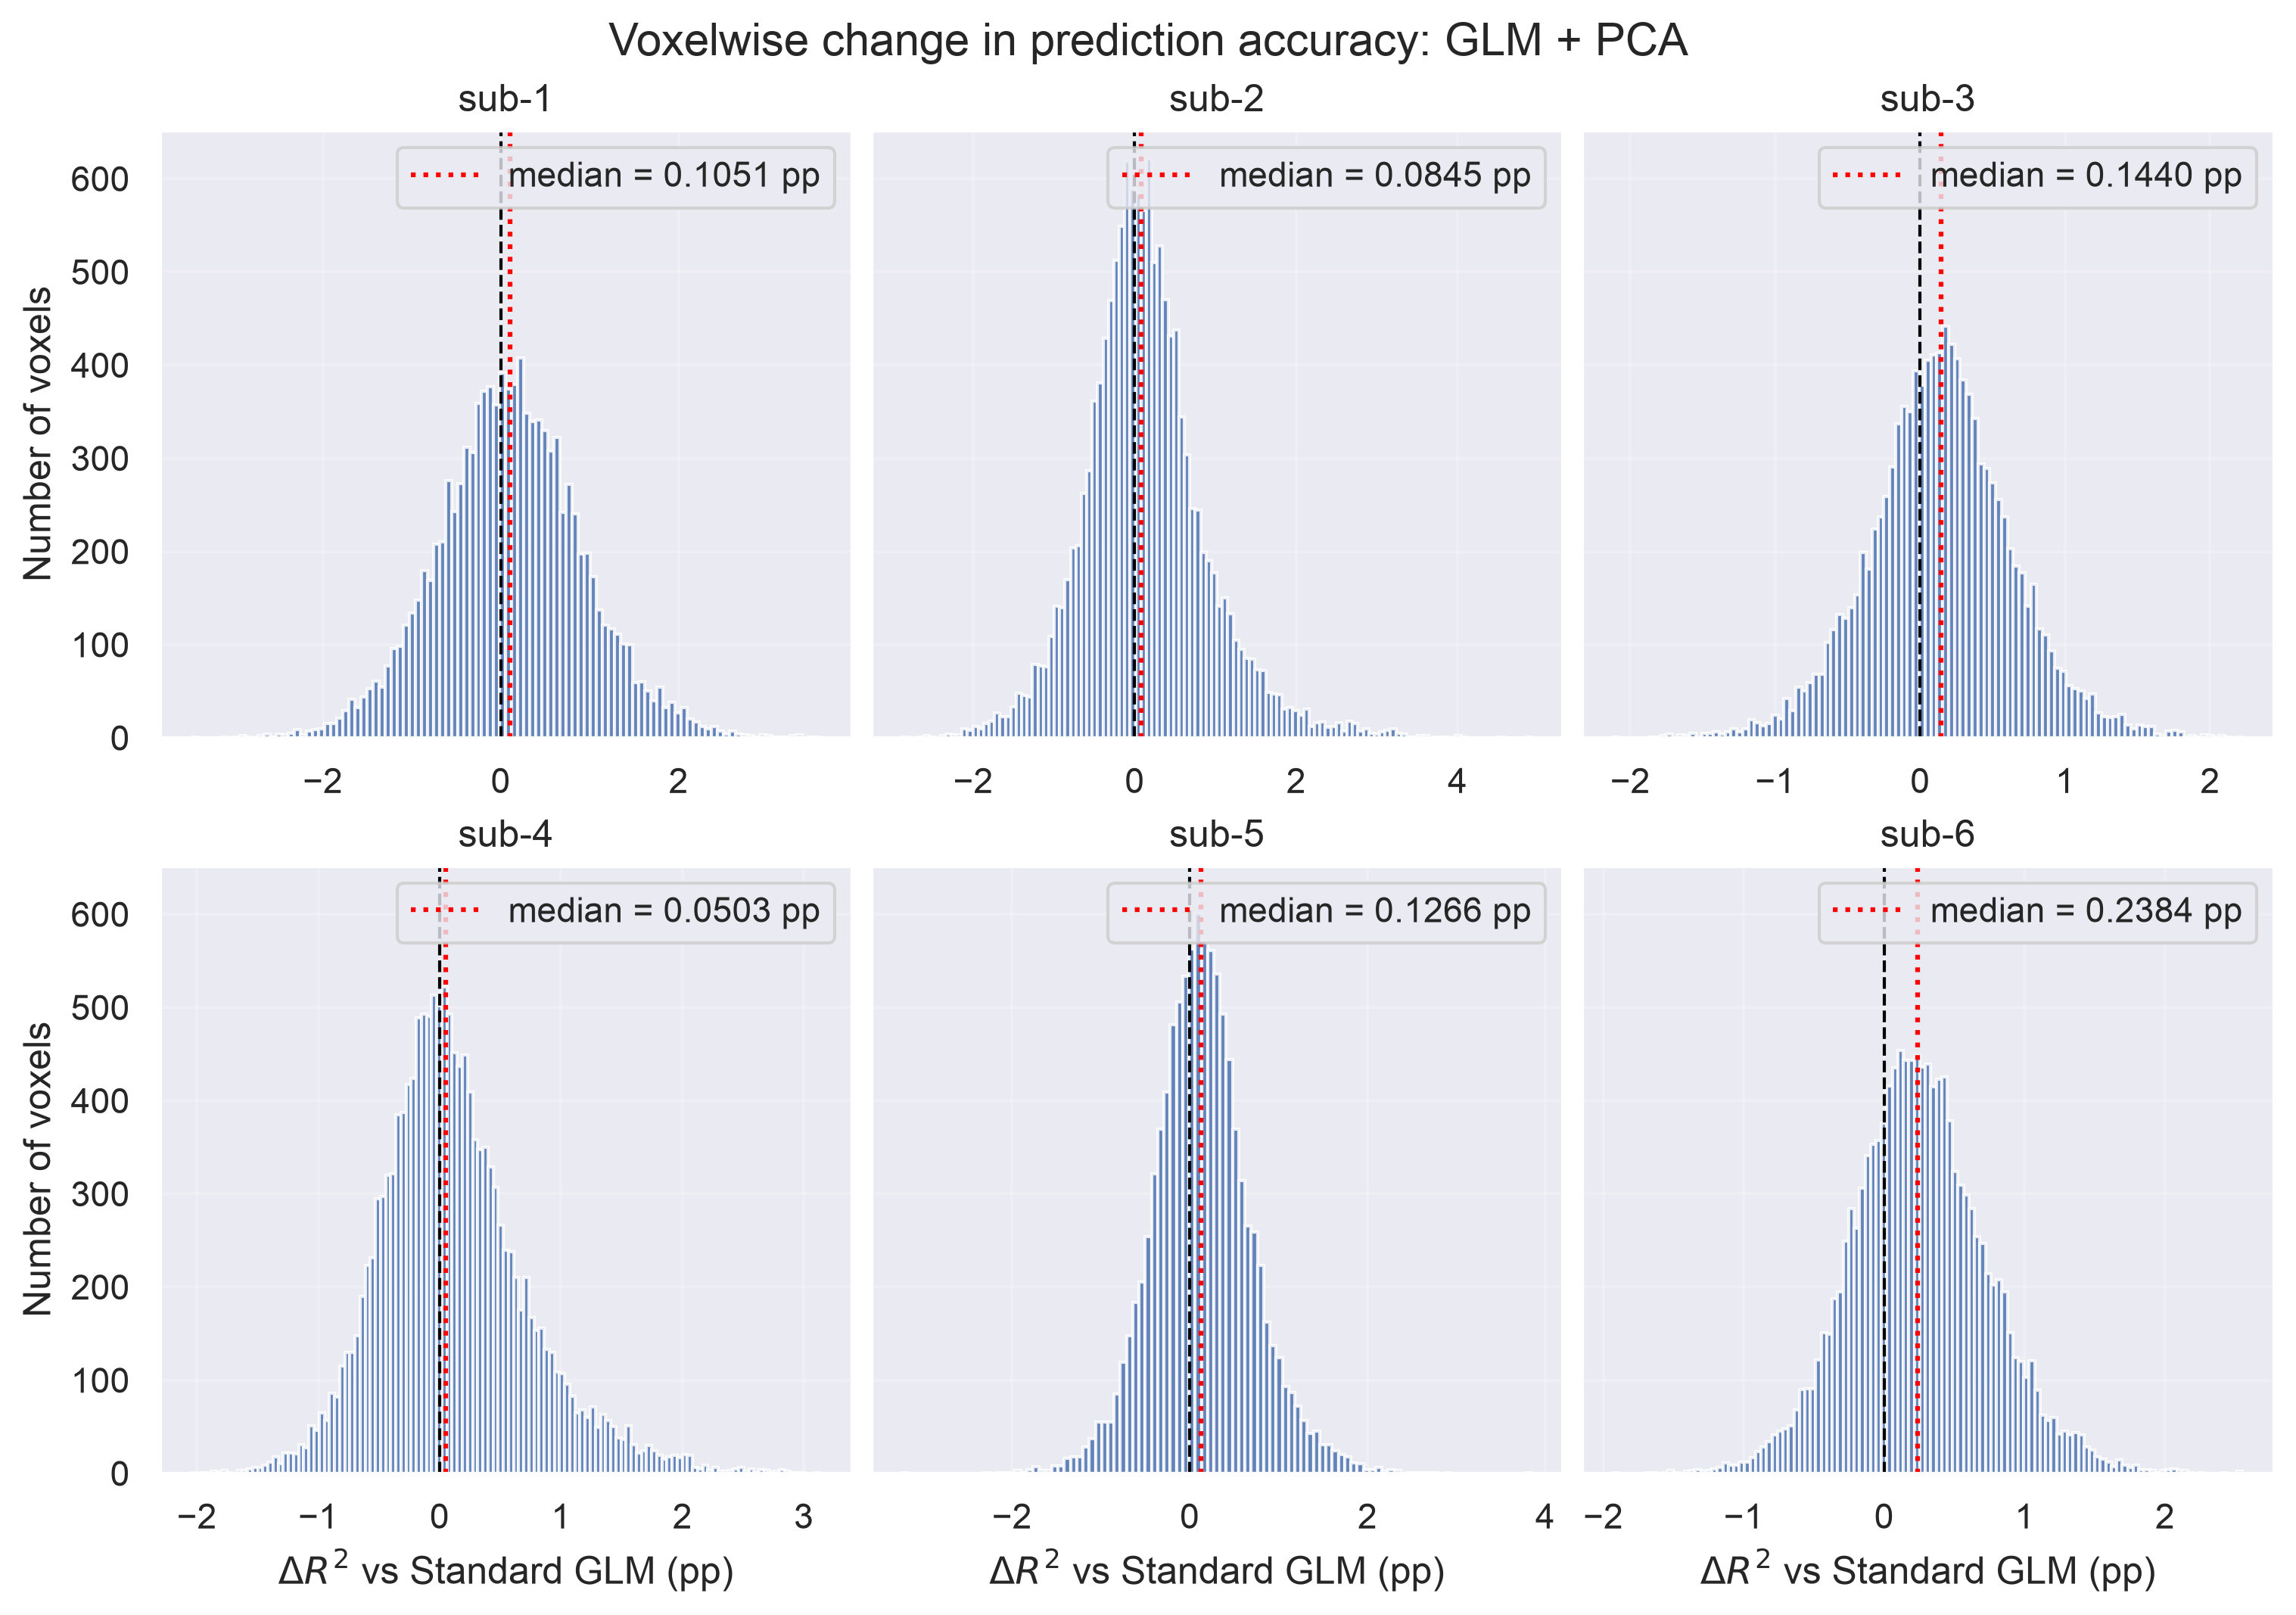
\includegraphics[scale=0.5]{fig/delta_r2_distribution_glm_pca.png}
    \caption{Distributions of voxelwise changes in outer-CV prediction accuracy for PCA-assisted GLM denoising relative to the standard GLM for each subject.}
    \label{fig:r2-distribution-glm-pca}
\end{figure}

\begin{figure}[!htbp]
    \centering
    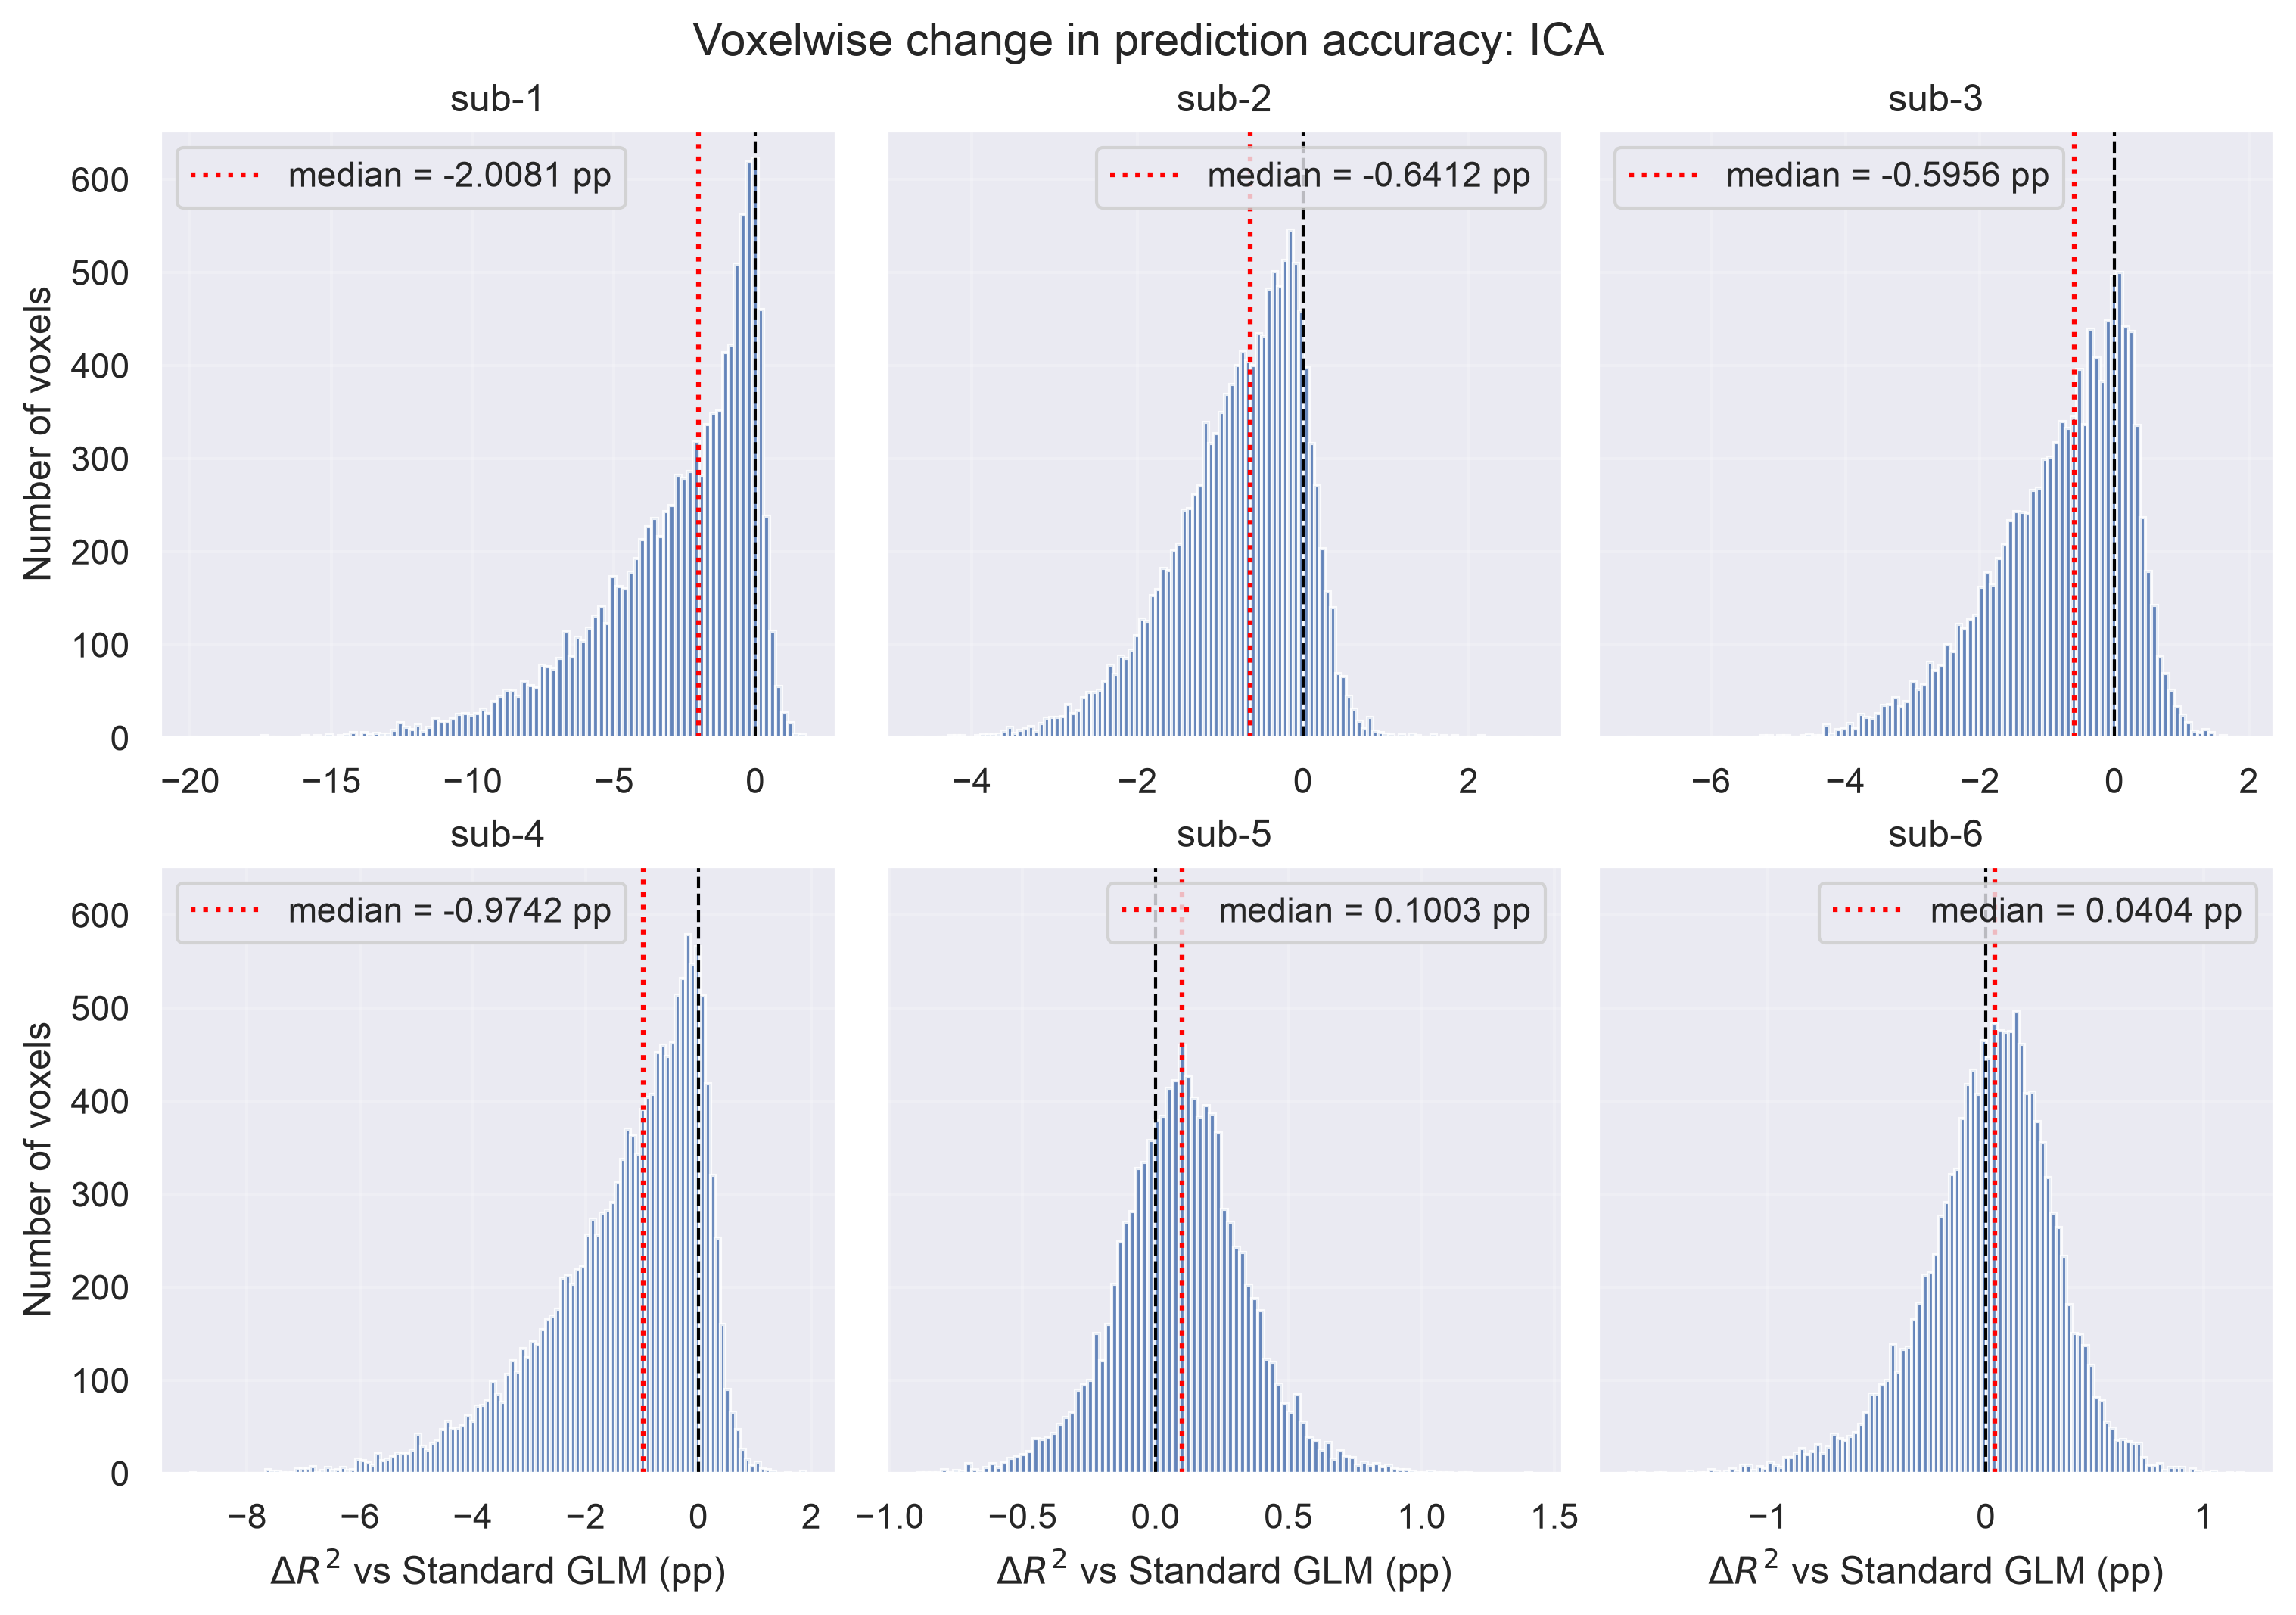
\includegraphics[scale=0.5]{fig/delta_r2_distribution_ica.png}
    \caption{Distributions of voxelwise changes in outer-CV prediction accuracy for ICA-based denoising relative to the standard GLM for each subject.}
    \label{fig:r2-distribution-ica}
\end{figure}

For readability, abbreviated labels are used in all subsequent figures. Subject labels such as \verb|sub-1| and \verb|sub-2| correspond to the original labels \verb|subject-1| and \verb|subject-2|, respectively. Method names are abbreviated in the same manner: \verb|Standard GLM| denotes the standard GLM, \verb|GLM+PCA| denotes the PCA-assisted GLM, and \verb|ICA| denotes the ICA-based denoising procedure. These abbreviations are used consistently throughout the remaining figures.

Figures~\ref{fig:r2-distribution-glm-pca}~and~\ref{fig:r2-distribution-ica} compare voxelwise outer-CV prediction accuracy of the PCA-assisted GLM denoising and ICA-based denoising, respectively, against the standard GLM for all participants. On each plot, the median is presented alongside a reference line corresponding to a difference of 0 percentage points. 
These distributions show how the voxelwise $\Delta R^2$ values described in Equation~\eqref{eq:delta-r2-standard} are distributed. Note that the horizontal axis is scaled independently for each subject to improve visualization of the distributional shape.

The most visible difference can be seen in the shape of these distributions. For PCA-assisted GLM denoising, the values are distributed on both sides of the $x=0$ line, with a slight shift towards positive values. Additionally, each median lies to the right of said line. Most of the plots have similar horizontal scales, approximately spanning $[-2, 2]$. Distributions for some subjects slightly exceed this range.
Conversely, for ICA-based denoising the majority of the distribution mass is located to the left of the $x=0$ line, except for distributions for subjects 5 and 6, which more resemble the distributional shapes of the PCA-assisted GLM denoising, having values distributed on both sides of the $x=0$ line. Additionally, these two subjects have positive median $\Delta R^2$ values and a similar horizontal axis scale in the range of $[-1, 1]$. For the remaining subjects (subjects 1--4), these scales differ considerably, most notably for the first subject, whose distribution spans approximately $[-20, 2]$. Median lines of these distributions also lie in the negative part of the plot, with the lowest median of approximately $-2$ percentage points belonging to the first subject.

These results show a small overall improvement in prediction accuracy for PCA-assisted GLM denoising relative to the standard GLM, as indicated by positive median $\Delta R^2$ values for all subjects. Some distributions are placed more to the right of the $x=0$ line (subjects~3,~5~and~6), indicating that the majority of the voxelwise $\Delta R^2$ values are positive, although the magnitude of the improvement remains small. All of the distributions show a strong concentration around their central values, while also containing relatively short tails. The best results can be seen for subject 6, where both the distribution, as well as the median are shifted to the right, suggesting the largest overall improvement in comparison with the standard GLM.

For ICA-based denoising the distributions mostly show a decline in prediction accuracy. Subjects 1--4 have a large majority of voxels to the left of the $x=0$ line, indicating that most of the voxelwise prediction accuracy differences are negative, meaning worse prediction accuracy than the standard GLM. The median values additionally reflect this conclusion, with the worst result appearing for the first participant. These distributions are also considerably more asymmetric than those obtained for PCA-assisted GLM denoising, with pronounced negative tails for subjects 1–4 and the most extreme negative tail observed for subject 1. The best results are for subjects 5 and 6, where the median lies to the right of the $x=0$ line, and the distributions are more symmetric around zero.

The results additionally indicate substantially greater between-subject variability for ICA-based denoising. While PCA-assisted GLM denoising produces small positive median changes for all participants, the effect of ICA-based denoising ranges from a considerable deterioration for subject 1 to approximately neutral or slightly positive changes for subjects 5 and 6.

Overall, these plots show the poorer predictive performance of ICA-based denoising in comparison with PCA-assisted GLM denoising and the standard GLM.

\begin{figure}[!htbp]
    \centering
    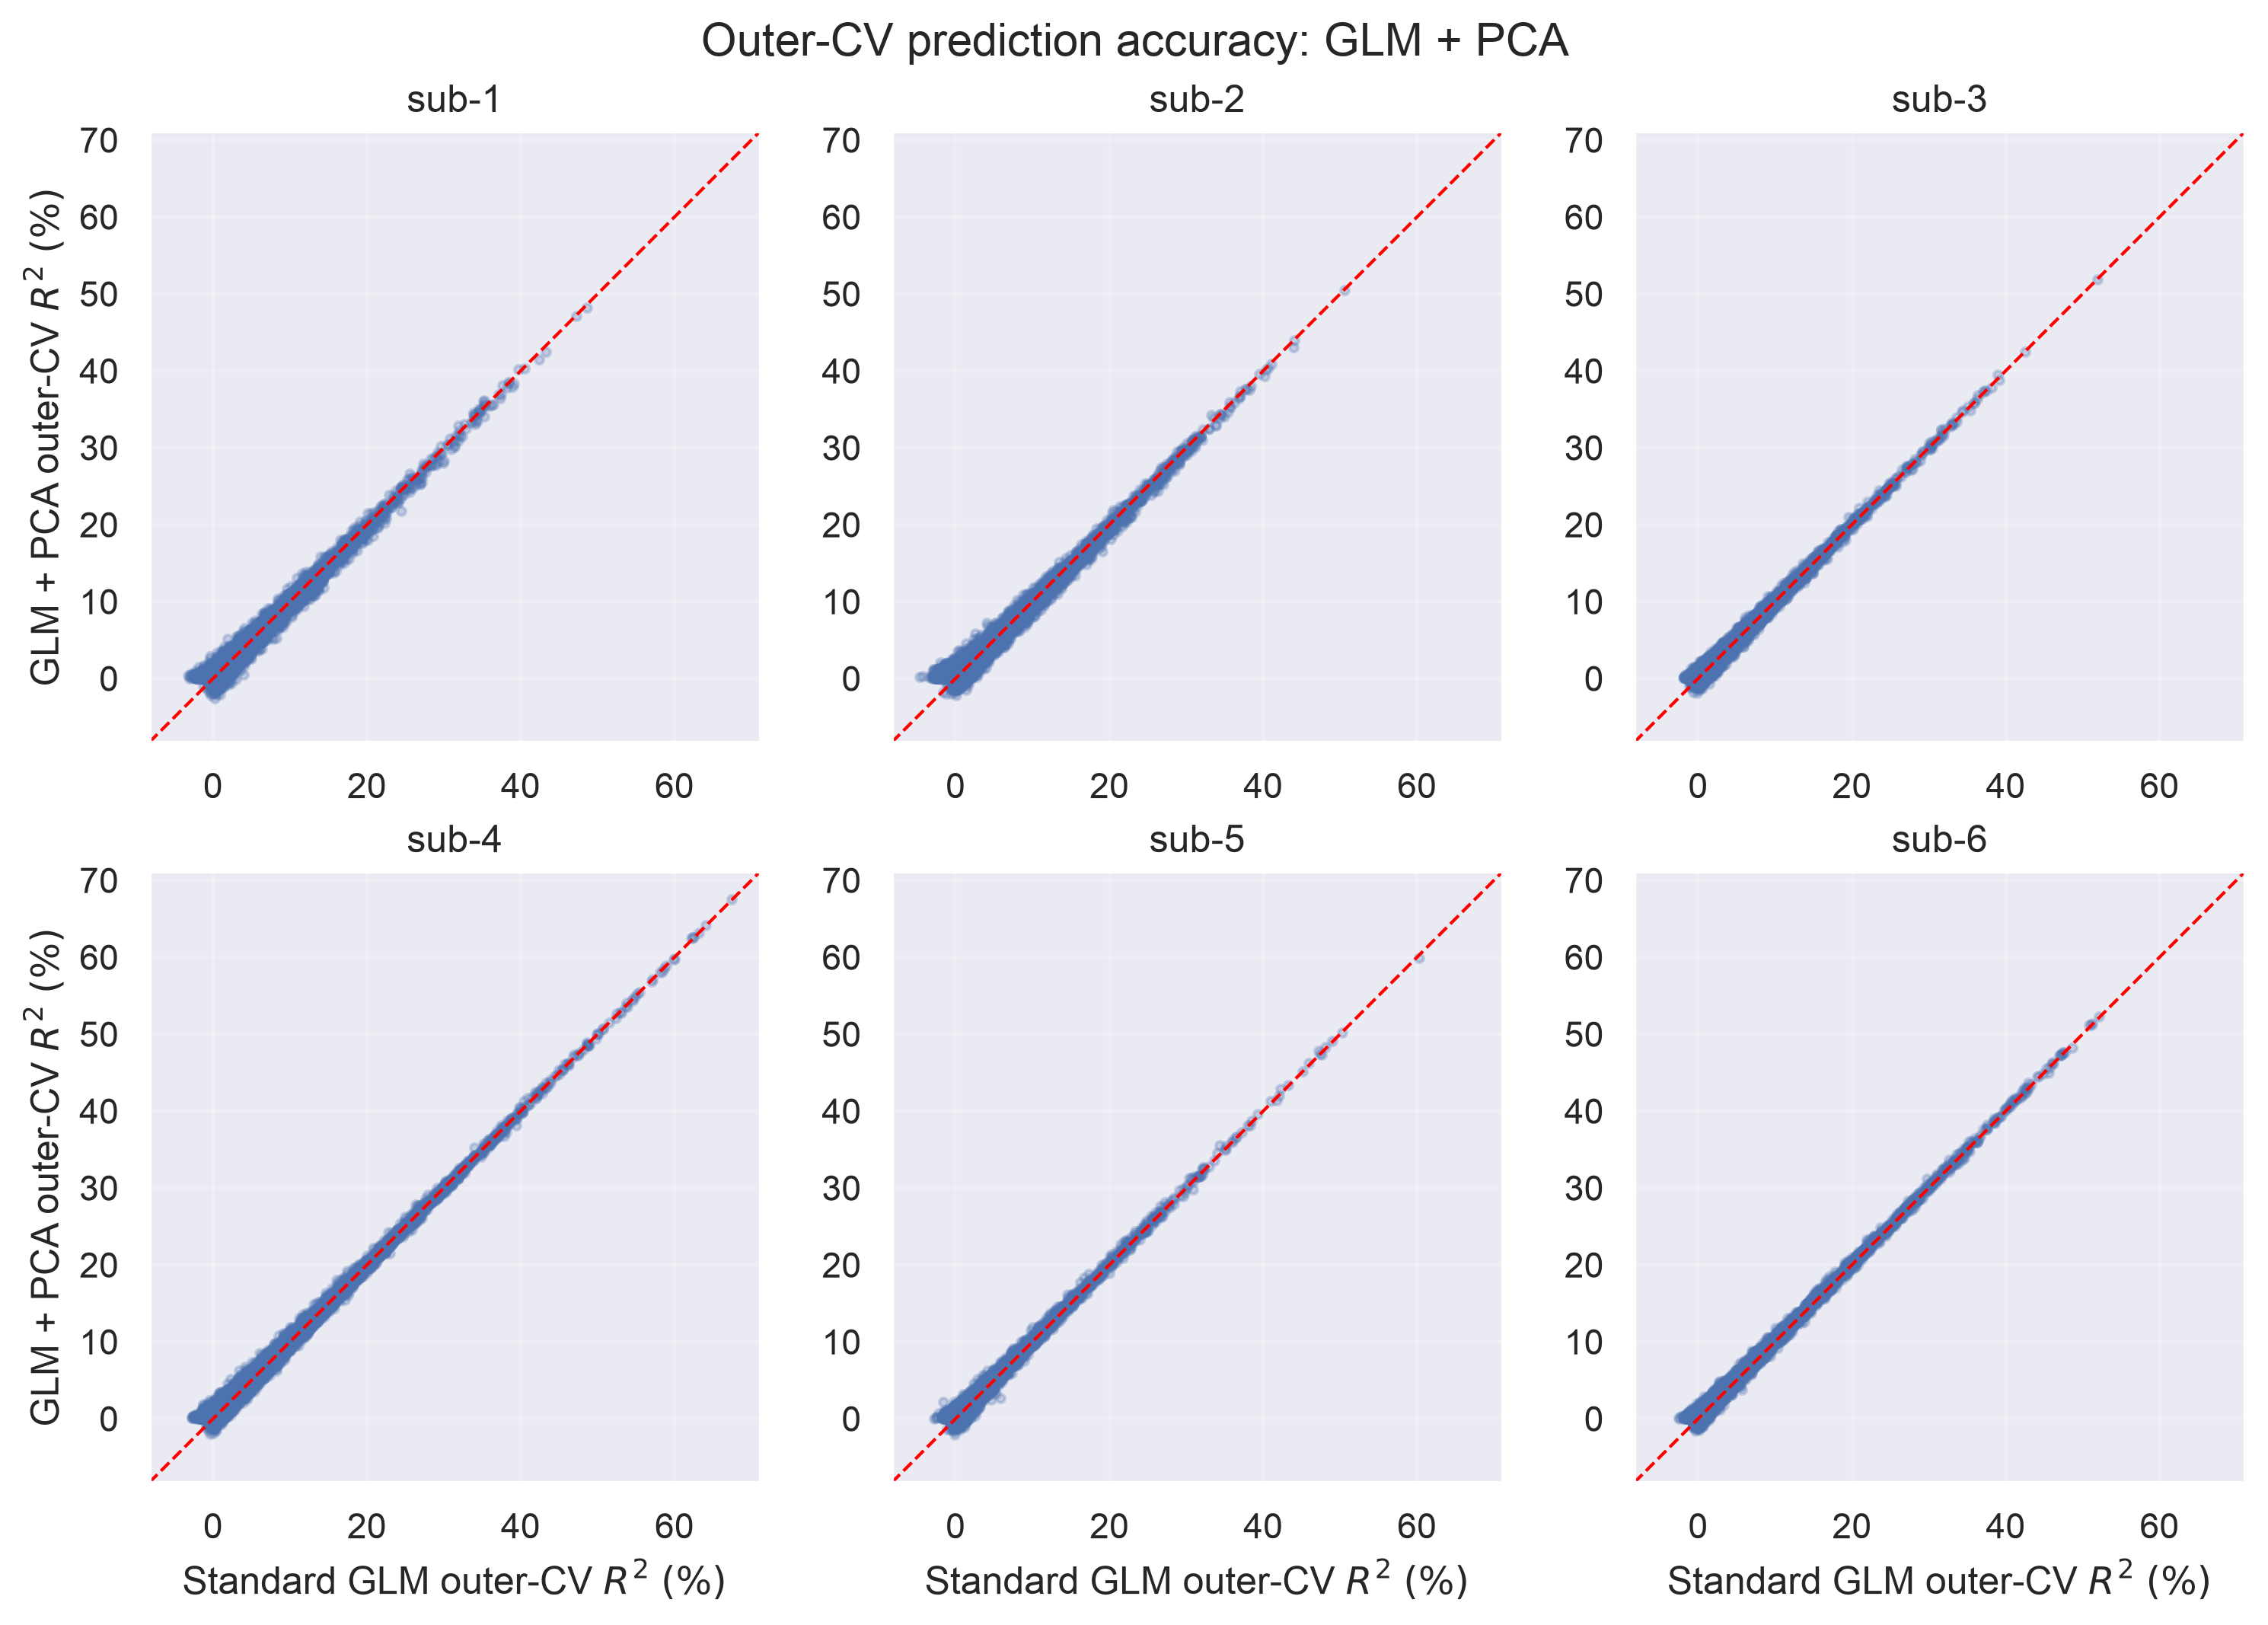
\includegraphics[scale=0.5]{fig/r2_scatter_glm_pca.png}
    \caption{Scatter plots of voxelwise outer-CV prediction accuracy for PCA-assisted GLM denoising relative to the standard GLM for each subject.}
    \label{fig:r2-voxelwise-glm-pca}
\end{figure}

\begin{figure}[!htbp]
    \centering
    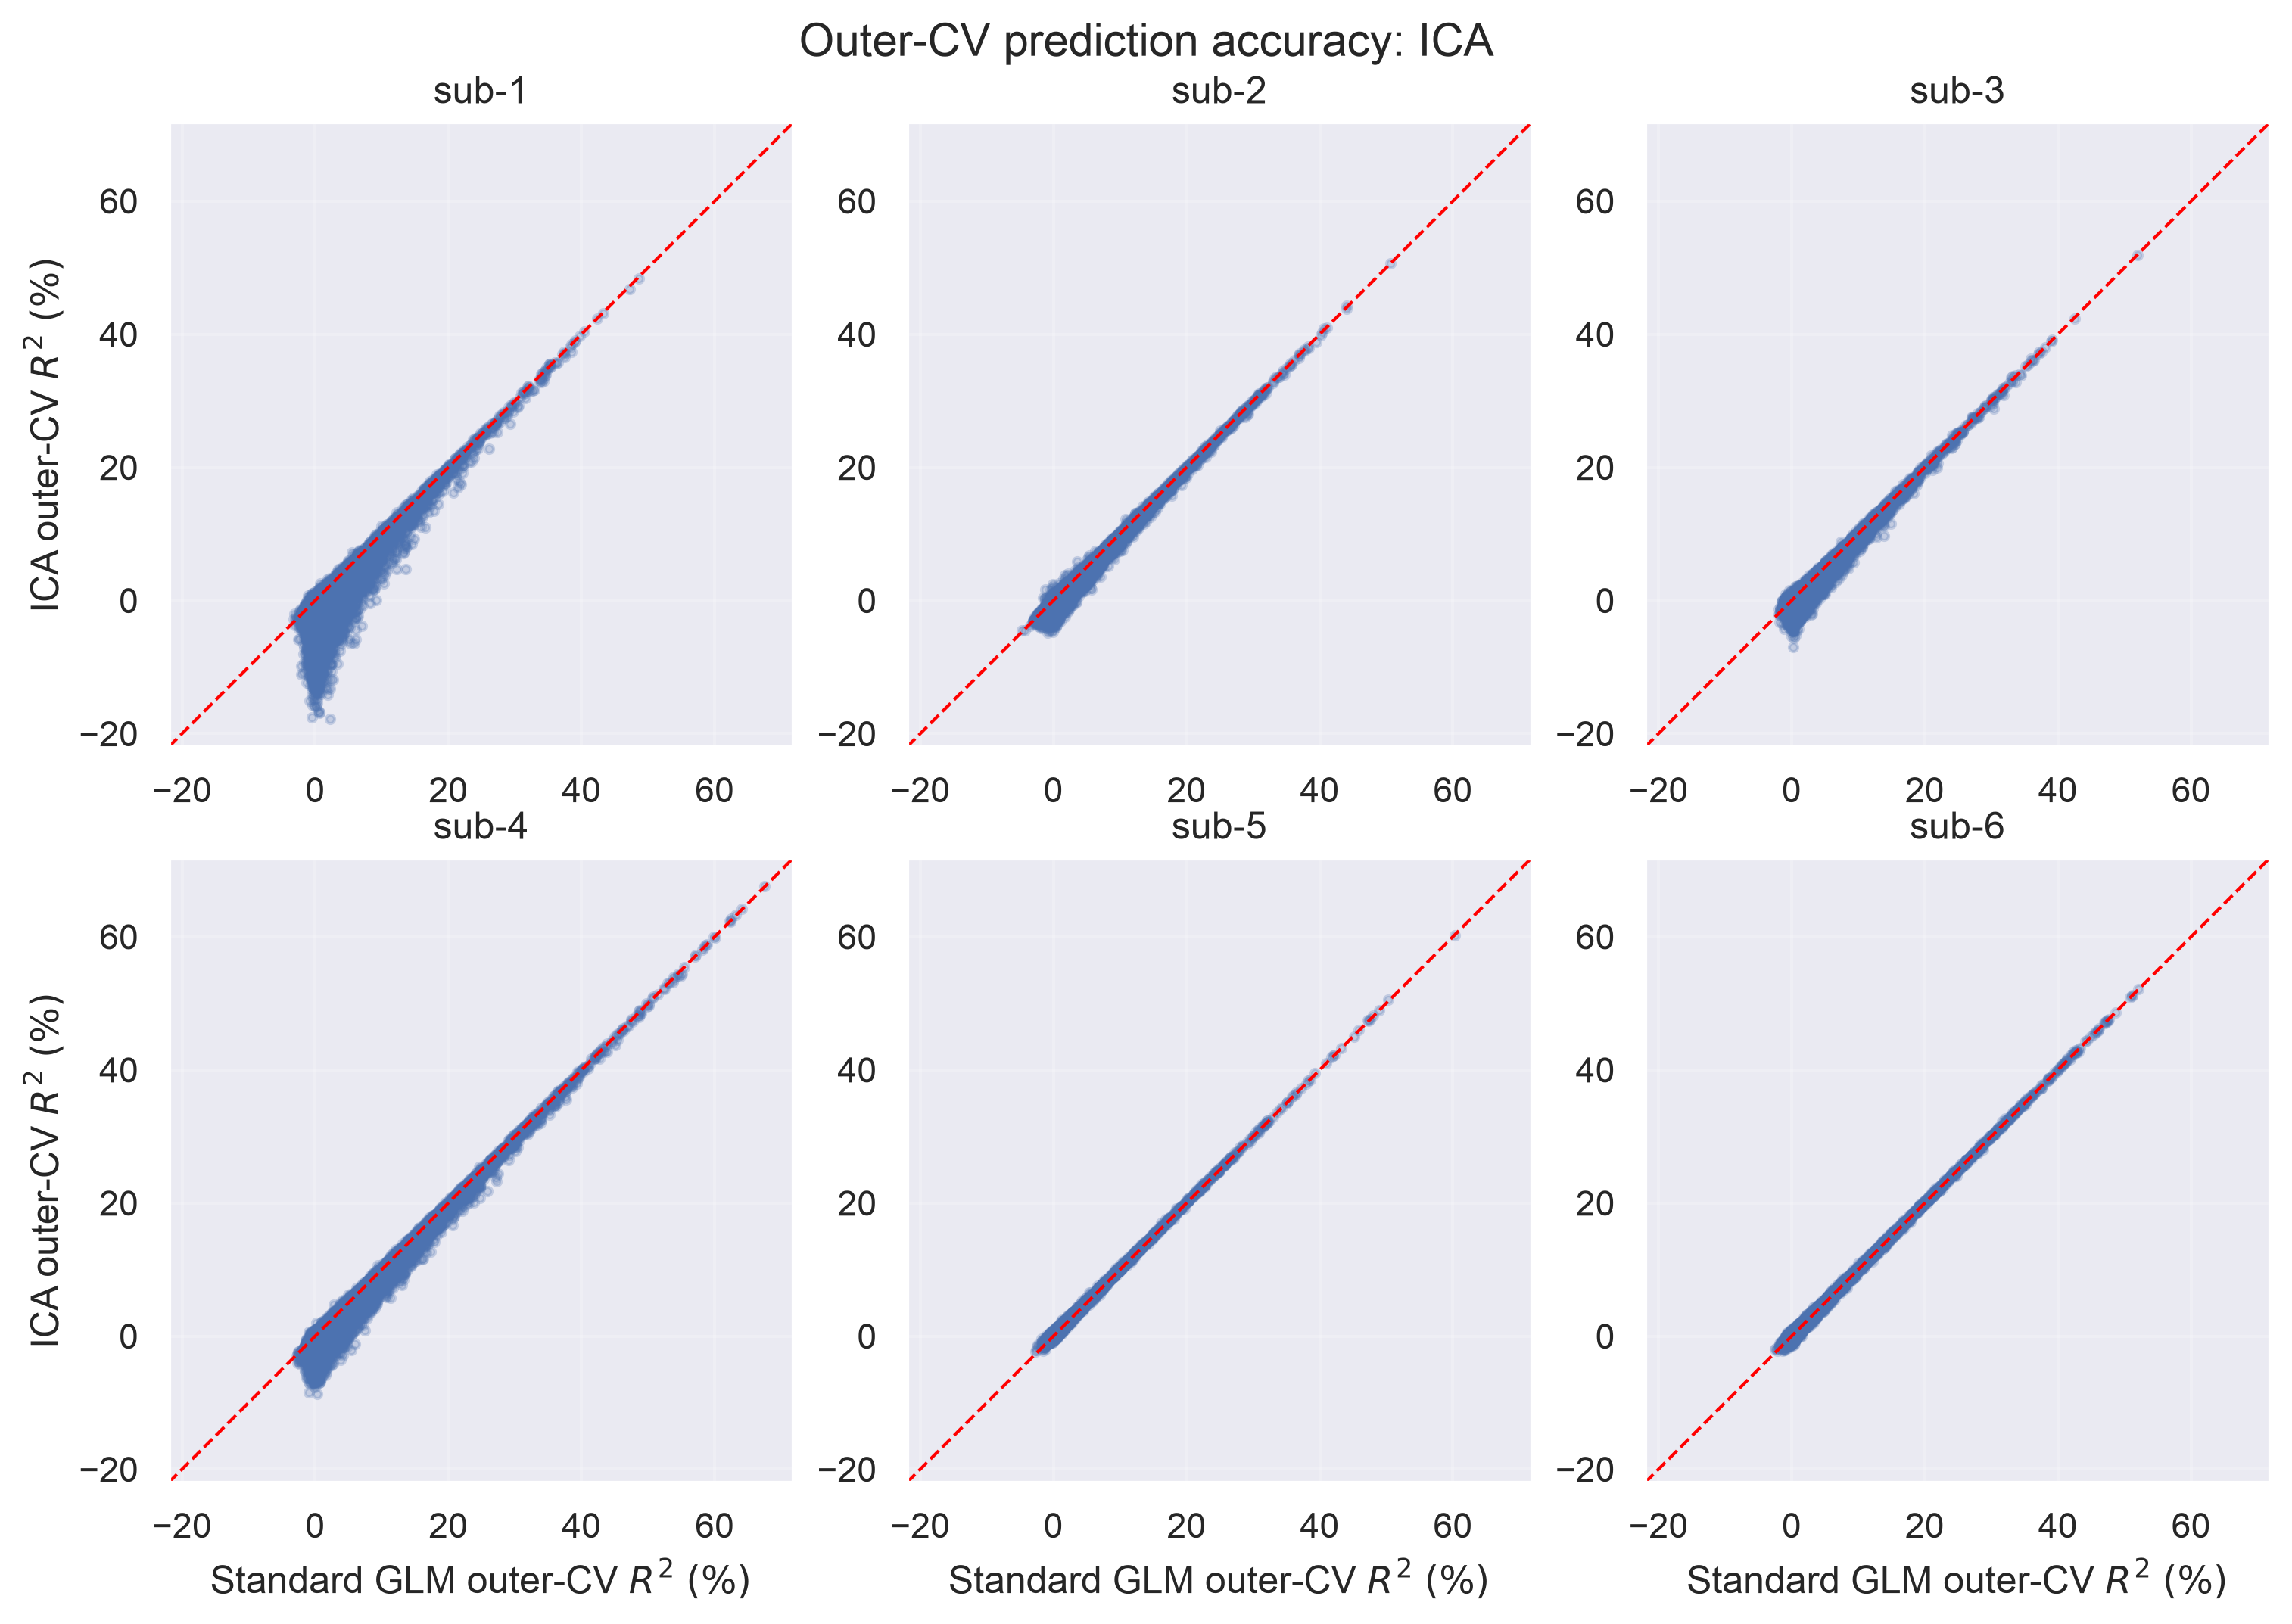
\includegraphics[scale=0.5]{fig/r2_scatter_ica.png}
    \caption{Scatter plots of voxelwise outer-CV prediction accuracy for ICA-based denoising relative to the standard GLM for each subject.}
    \label{fig:r2-voxelwise-ica}
\end{figure}

Figures~\ref{fig:r2-voxelwise-glm-pca}~and~\ref{fig:r2-voxelwise-ica} present voxelwise outer-CV prediction accuracy relative to the standard GLM and are analogous to \cite[Figure 4A]{glm-denoise}. The plots show pairs of $R^2$ values expressed as percentages. For each voxel, the $x$-coordinate corresponds to the prediction accuracy obtained with the standard GLM, while the $y$-coordinate corresponds to the prediction accuracy obtained with PCA-assisted GLM denoising or ICA-based denoising in Figures~\ref{fig:r2-voxelwise-glm-pca}~and~\ref{fig:r2-voxelwise-ica}, respectively. The identity line represents equal prediction accuracy for the two compared methods. Points below the line indicate lower outer-CV $R^2$ relative to the standard GLM, whereas points above the line indicate an improvement. These plots provide a complementary representation of the results shown by the distributions in~Figures~\ref{fig:r2-distribution-glm-pca}~and~\ref{fig:r2-distribution-ica}.

Results comparing the PCA-assisted GLM with the standard GLM are presented in Figure~\ref{fig:r2-voxelwise-glm-pca} and show a consistent pattern across subjects. For most voxels, the points are concentrated close to the identity line, indicating only small differences in outer-CV prediction accuracy between the two methods. The highest density of points occurs at lower baseline $R^2$ values, where the scatter is also somewhat wider, indicating greater variability in the effect of the PCA-derived nuisance regressors. For subject 2, voxels with low baseline $R^2$ values show a slight tendency to lie above the identity line, suggesting a modest improvement under the PCA-assisted GLM. This tendency becomes less pronounced as baseline prediction accuracy increases, with the points becoming increasingly concentrated around the identity line. Across all subjects, voxels with high outer-CV $R^2$ values are less numerous and more sparsely distributed. Overall, the results indicate that the PCA-assisted GLM generally preserves the predictive performance of the standard GLM while providing only small voxelwise improvements, consistent with the distributions presented in Figure~\ref{fig:r2-distribution-glm-pca}.

\newpage
The pattern of poorer predictive performance of ICA-based denoising can again be observed in Figure~\ref{fig:r2-voxelwise-ica}. For subjects 1--4, a substantial proportion of voxels lies below the identity line, indicating lower outer-CV $R^2$ values than those obtained with the standard GLM. This effect is most pronounced for subject 1, where a wide downward deviation from the identity line is visible for voxels with low and moderate baseline prediction accuracy. For these subjects, the discrepancy between ICA and the standard GLM decreases for voxels with higher baseline $R^2$, whose values remain closer to the identity line. In contrast, subjects 5 and 6 exhibit points concentrated almost entirely around the identity line, indicating that ICA-based denoising produces little change in prediction accuracy for these participants.

Therefore, the scatter plots support the conclusions obtained from the voxelwise $\Delta R^2$ distributions: PCA-assisted GLM denoising produces small but relatively consistent changes across subjects, whereas the effect of ICA-based denoising is substantially more subject-dependent and can lead to considerable deterioration in voxelwise prediction accuracy.

\begin{figure}[!htbp]
    \centering
    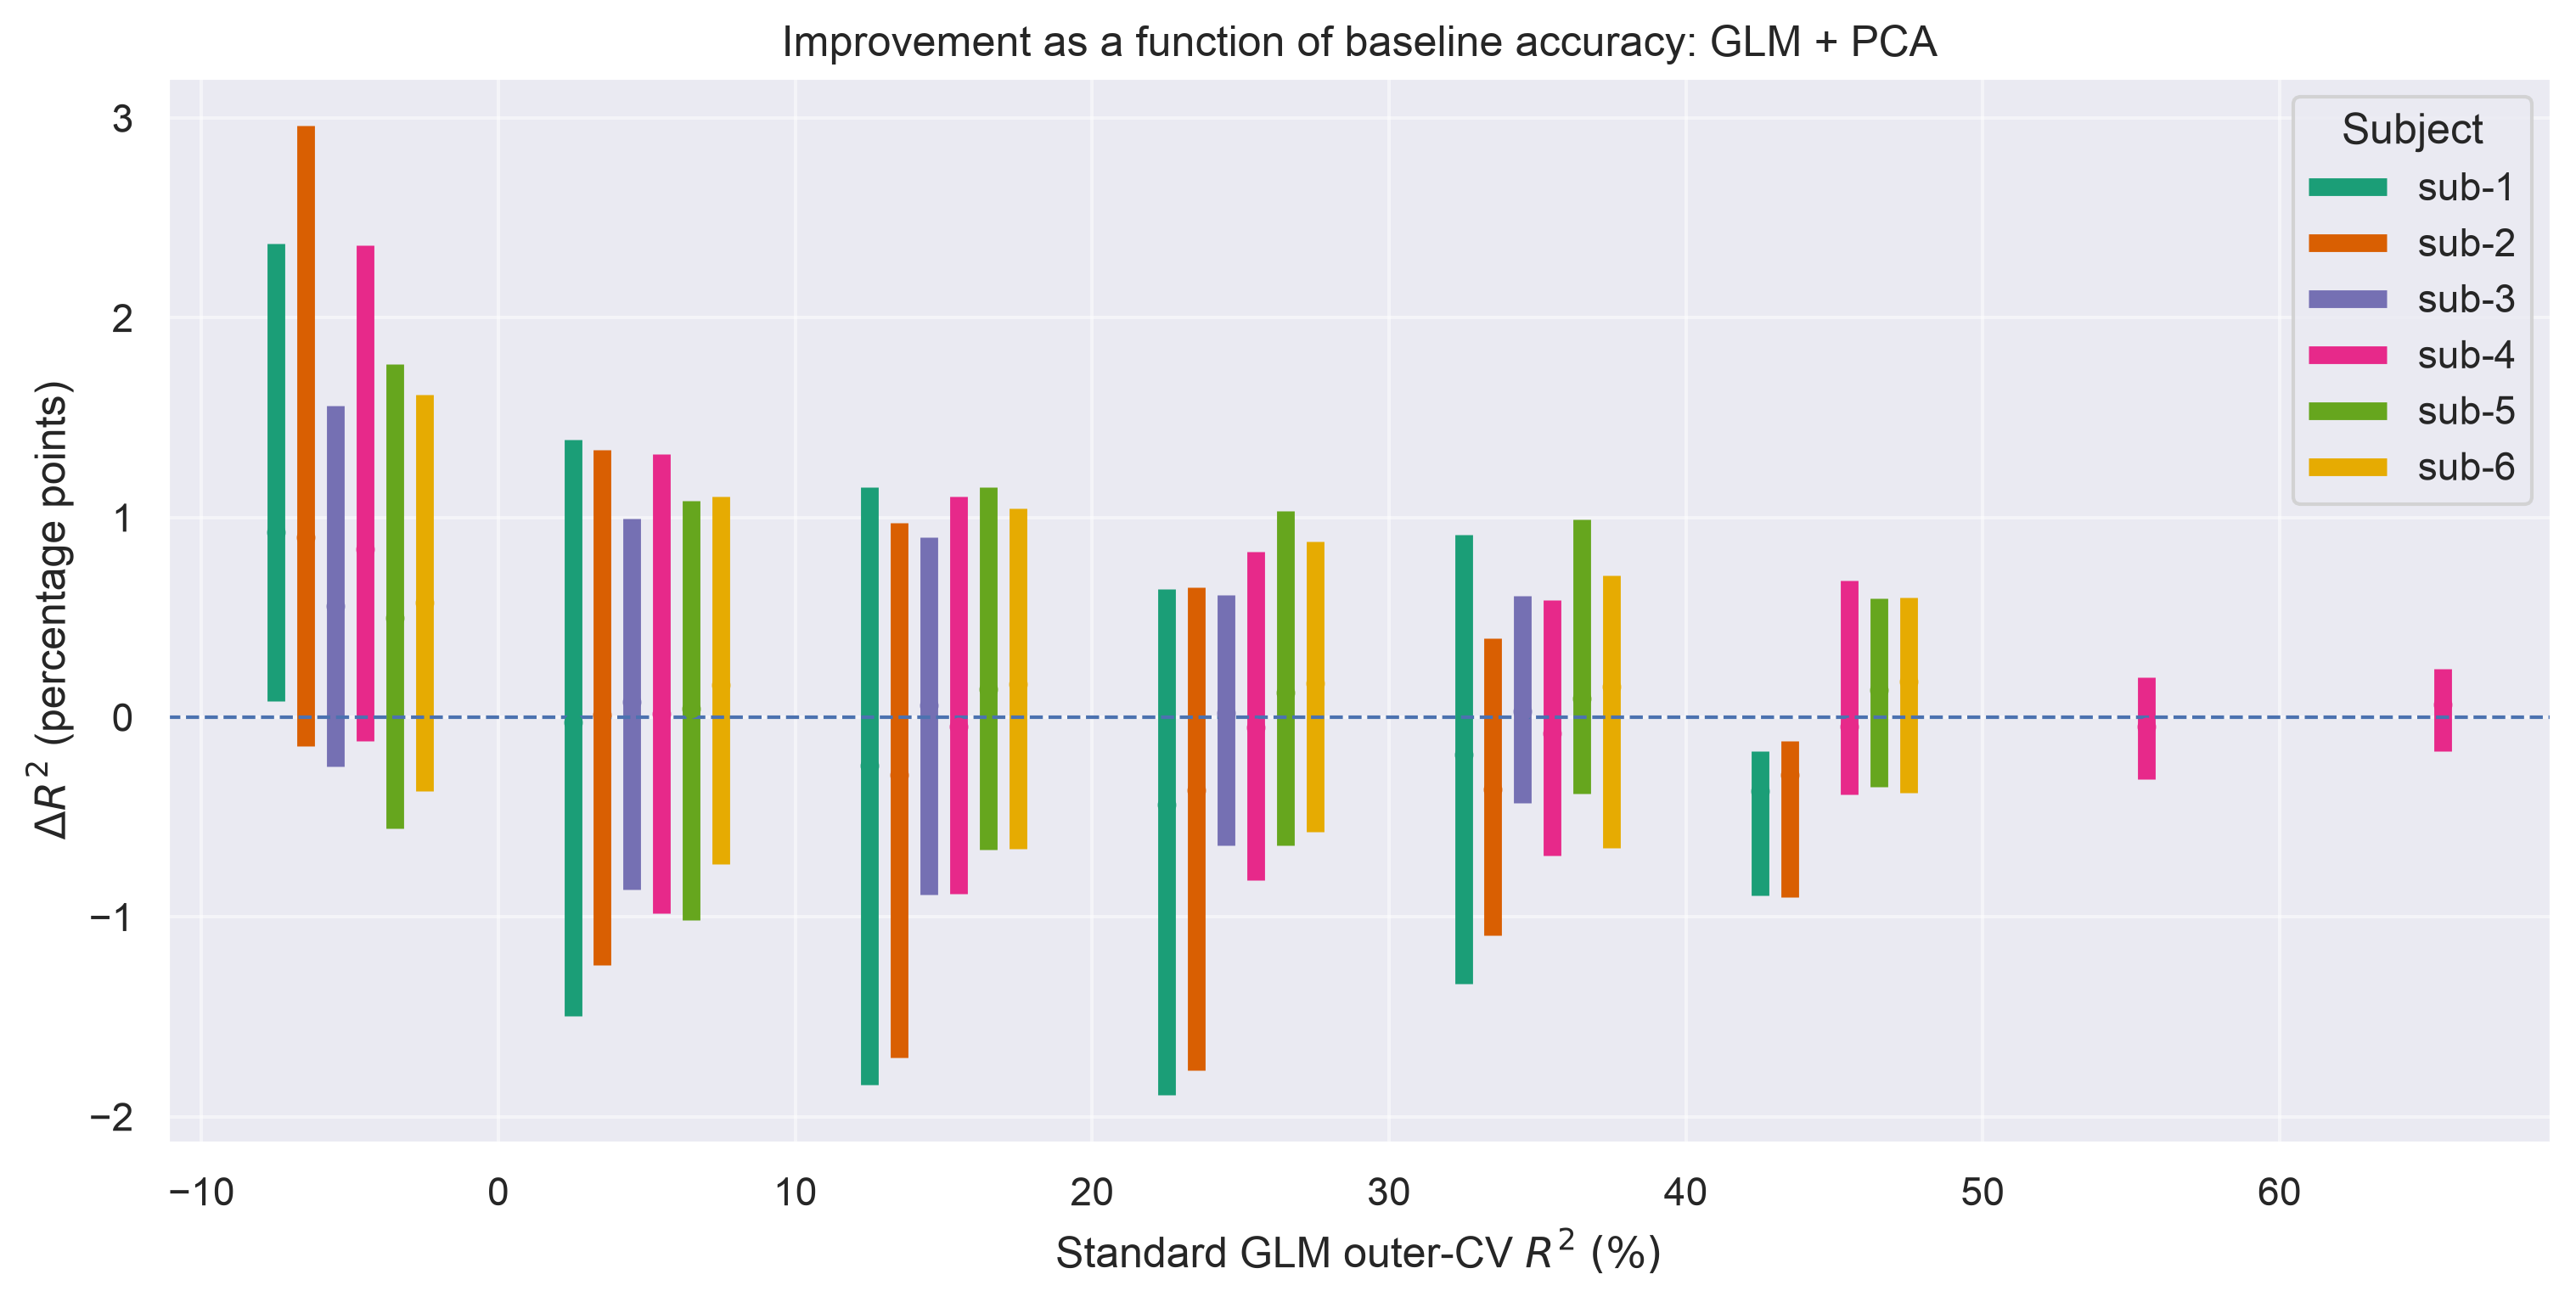
\includegraphics[scale=0.5]{fig/r2_improvement_binned_glm_pca.png}
    \caption{Voxelwise change in outer-CV prediction accuracy for PCA-assisted GLM relative to the standard GLM, summarized within 10-percentage-point baseline $R^2$ bins by the $95\%$ range for each subject.}
    \label{fig:r2-binned-glm-pca}
\end{figure}
\begin{figure}[!htbp]
    \centering
    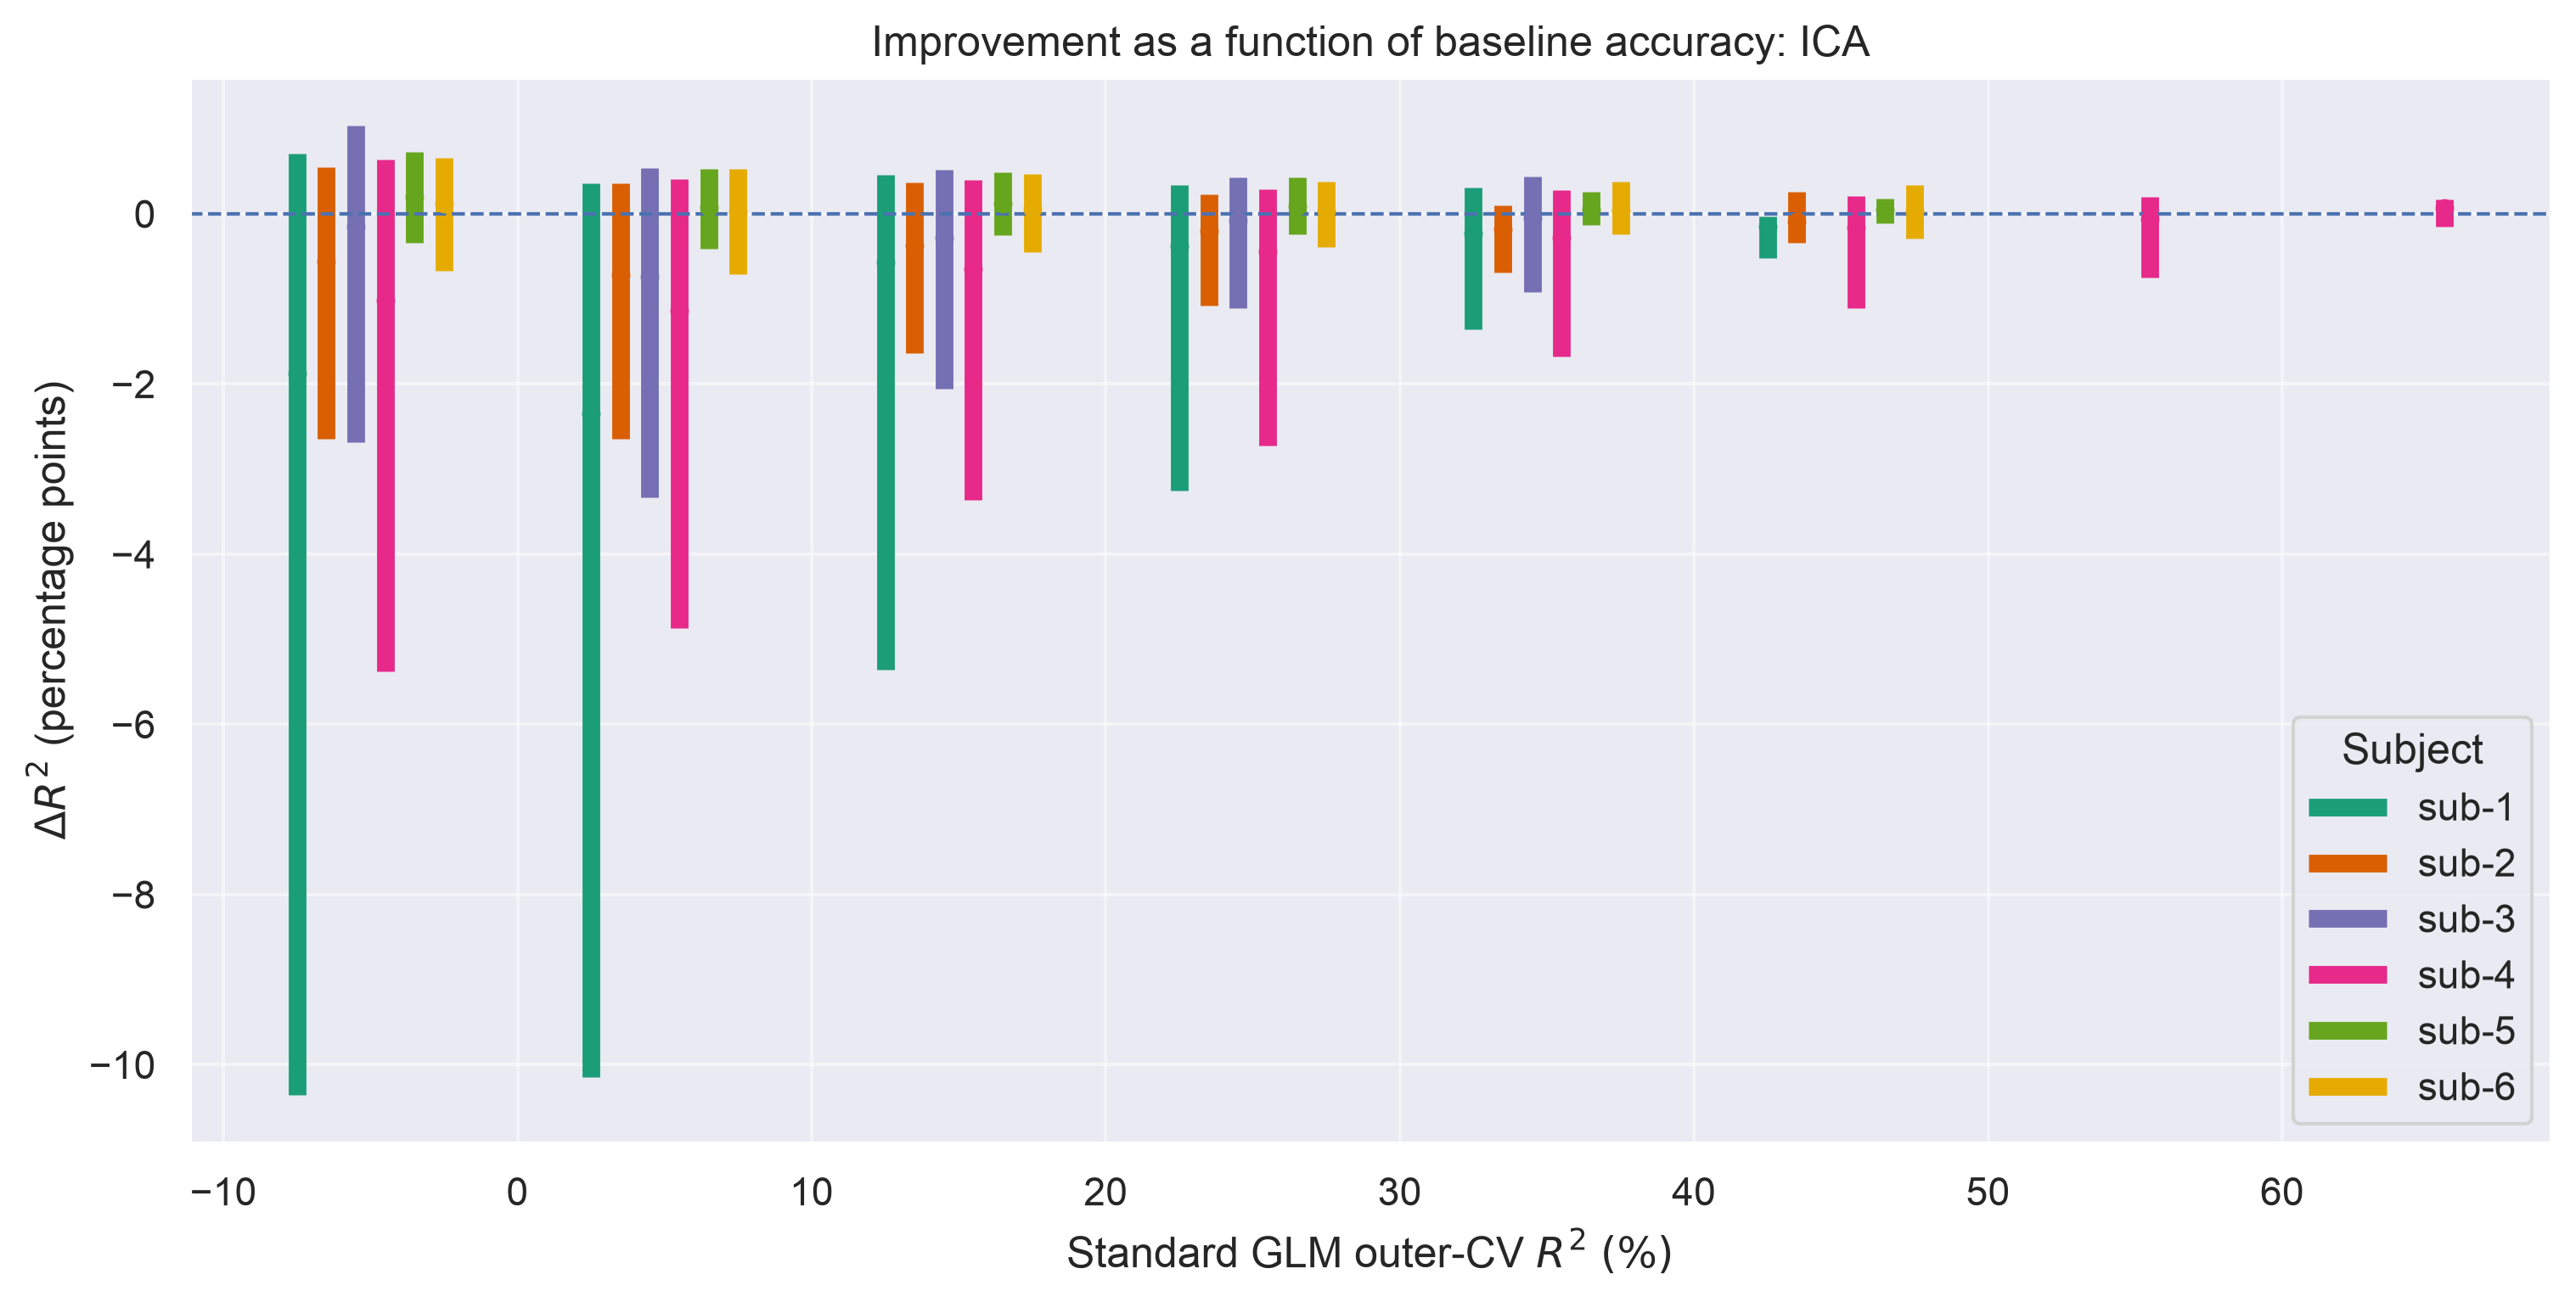
\includegraphics[scale=0.5]{fig/r2_improvement_binned_ica.png}
    \caption{Voxelwise change in outer-CV prediction accuracy for ICA relative to the standard GLM, summarized within 10-percentage-point baseline $R^2$ bins by the $95\%$ range for each subject.}
    \label{fig:r2-binned-ica}
\end{figure}

For further analysis of improvement of prediction accuracy relative to standard GLM denoising, Figures~\ref{fig:r2-binned-glm-pca}~and~\ref{fig:r2-binned-ica} were produced. These figures present voxelwise changes in outer-CV prediction accuracy as a function of the prediction accuracy obtained with the standard GLM. Voxels are grouped into bins of width 10 percentage points according to their standard GLM outer-CV $R^2$. For each subject and each bin, the $95\%$ range of voxelwise $\Delta R^2$ values is presented. These plots are analogous to \cite[Figure 4B]{glm-denoise}. They therefore show how the effect of each denoising method depends on the baseline prediction accuracy of the corresponding voxels.

For PCA-assisted GLM denoising, the largest positive changes can be observed among voxels for which the standard GLM obtains negative or low outer-CV $R^2$ values. Across subjects, the distributions within these bins generally extend further into the positive range. As the standard GLM $R^2$ increases, the ranges of $\Delta R^2$ values become narrower and increasingly concentrated around zero, indicating that PCA-assisted denoising has less influence on voxels that are already predicted relatively well by the standard GLM. This pattern is visible across baseline $R^2$ values in the approximate range $[-10\%,50\%)$. 
\newline
Above this range bins are present only for a subset of subjects, most notably subject 4. Subjects 1 and 2 additionally exhibit wider and more negative lower ranges than the remaining subjects for several bins above $10\%$ baseline $R^2$, and their $[40\%,50\%)$ ranges lie mostly below zero. Overall, however, the changes remain relatively small and centered close to zero for voxels with moderate or high baseline prediction accuracy.

ICA-based denoising again reflects poorer prediction accuracy in comparison with the standard GLM. For subjects 1--4, the $95\%$ ranges within most baseline-$R^2$ bins extend predominantly below zero, indicating that ICA frequently reduces voxelwise prediction accuracy. The strongest deterioration is observed for subject 1, particularly among voxels with negative or low standard GLM $R^2$, where the lower end of the range reaches approximately $-10$ percentage points. As baseline prediction accuracy increases, the magnitude and spread of these negative changes generally decrease, and the ranges approach zero. In contrast, subjects 5 and 6 show much smaller changes, with ranges located close to zero and extending into positive values across most bins. This behavior is consistent with the previous analyses, in which ICA-based denoising substantially degraded prediction accuracy for subjects 1--4 while producing approximately neutral results for subjects 5 and 6.

\begin{figure}[!htbp]
    \centering
    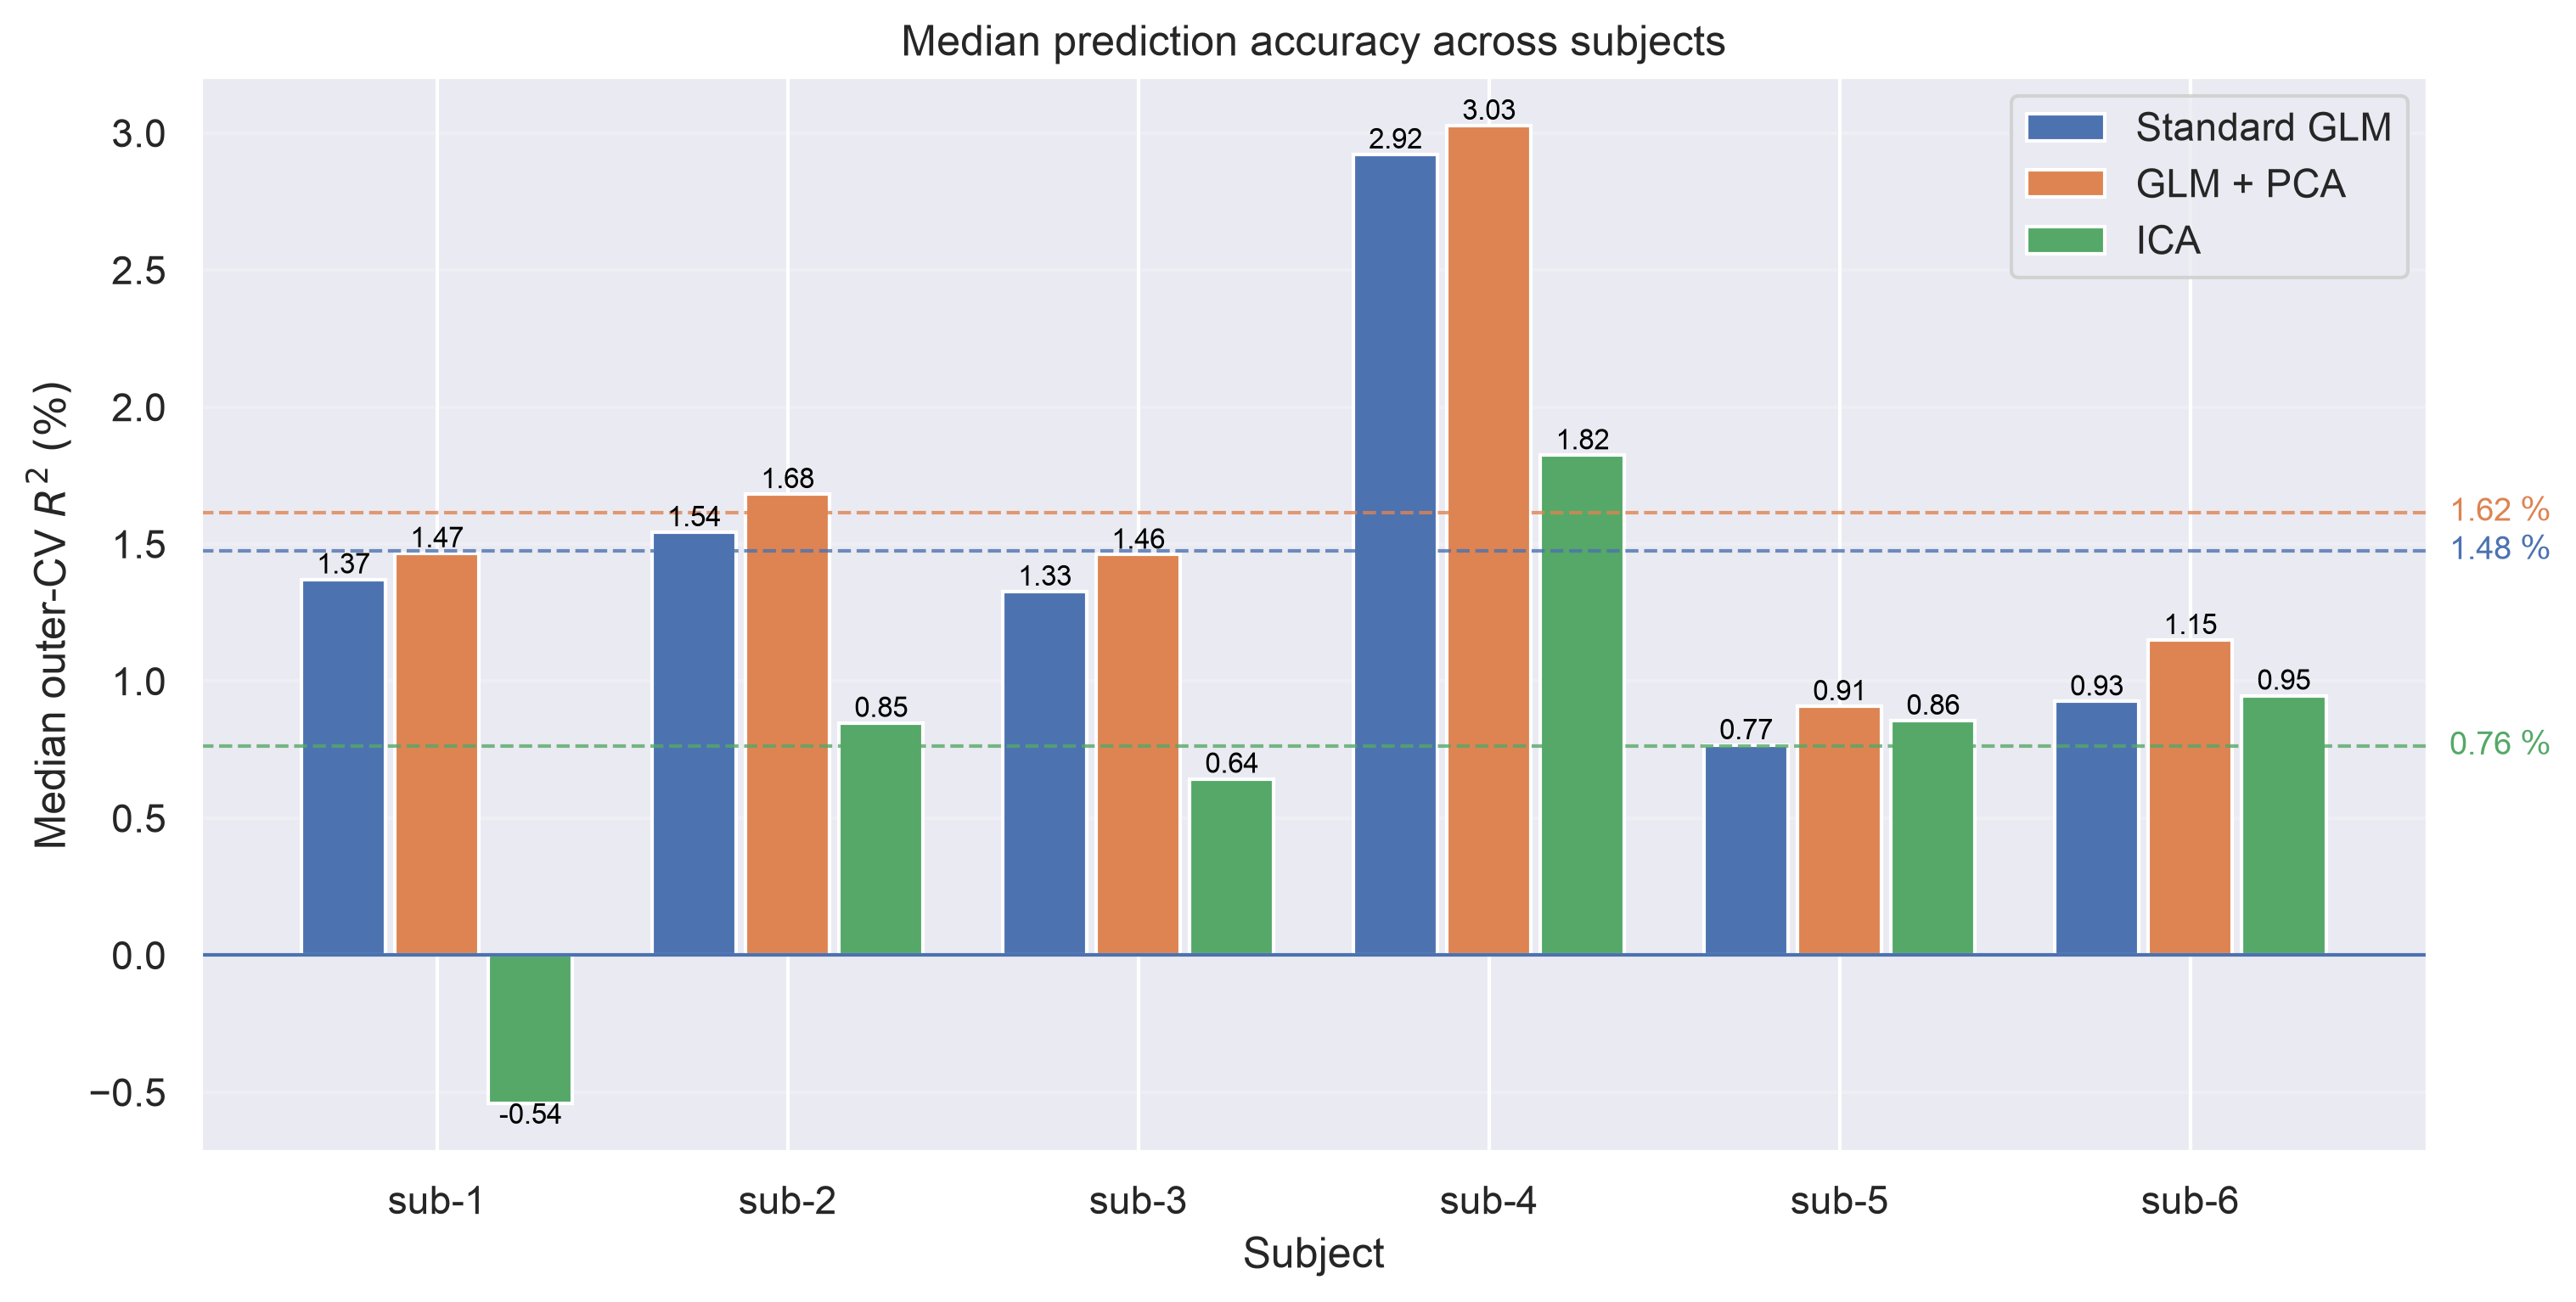
\includegraphics[width=\textwidth]{fig/median_r2.png}
    \caption{Median voxelwise outer-CV prediction accuracy for the standard GLM, PCA-assisted GLM denoising, and ICA-based denoising across subjects with mean median line for each method.}
    \label{fig:median-r2}
\end{figure}

To conclude the prediction accuracy analysis, Figure~\ref{fig:median-r2} focuses on the overall median outer-CV $R^2$ for the analyzed methods across subjects. Each subject is represented by three bars corresponding to the standard GLM, PCA-assisted GLM and ICA-based denoising. The medians are calculated across the candidate voxels included in the prediction accuracy analysis. Additionally, three horizontal lines show the mean of the subject-specific median $R^2$ values for each method.

PCA-assisted GLM denoising achieves the highest median prediction accuracy for all subjects. All median $R^2$ values are positive, with the highest value of $3.03 \%$ obtained for subject 4 and the lowest value of $0.91 \%$ for subject 5. However, improvement relative to the standard GLM remains small for every subject.

\newpage
Averaging the subject-specific median values further summarizes this pattern. The mean of the median outer-CV $R^2$ values is $1.62\%$ for PCA-assisted GLM denoising, compared with $1.48\%$ for the standard GLM, corresponding to an average difference of approximately $0.14$ percentage points.

The lowest values are mostly obtained for ICA-based denoising. For subjects 1--4, ICA has the lowest median $R^2$ among the three methods, with the poorest result of $-0.54\%$ observed for subject 1. In contrast, ICA slightly outperforms the standard GLM for subjects 5 and 6, by approximately $0.09$ and $0.02$ percentage points, respectively.

The mean of the subject-specific median outer-CV $R^2$ values for ICA-based denoising is $0.76\%$, which is approximately $0.72$ percentage points lower than the corresponding standard GLM value of $1.48\%$. This confirms the poorer overall prediction accuracy of ICA-based denoising.

The standard GLM generally provides the second-highest prediction accuracy. It is outperformed by PCA-assisted GLM denoising by a relatively small margin for every subject.

Overall, the median outer-CV $R^2$ values are relatively small, ranging from $-0.54\%$ to $3.03\%$, which is consistent with the low voxelwise prediction accuracy observed throughout the preceding analysis. ICA-based denoising generally performs worse than the standard GLM, particularly for subjects 1--4, whereas PCA-assisted GLM denoising provides a small but consistent improvement in prediction accuracy.

The potential reasons for these results are discussed in detail in Section~\ref{section:results-remarks}.

\newpage
\section{Method-specific component analysis}

Out of the selected methods, PCA-assisted GLM and ICA-based denoising both utilize Principal Component Analysis. The choice of the number of components is crucial, since it controls the amount of information retained or introduced by the respective procedures. However both of the analyzed methods perform the PCA for a different reason and on a different sets. The PCA-assisted GLM method uses PCA to construct additional nuisance regressors for the design matrix, as described in Section~\ref{section:pca-regressors}, while PCA in ICA-based denoising is used to reduce the data to a selected lower-dimensional subspace prior to ICA estimation, as described in Section~\ref{section:pica}. Additionally, the PCA-assisted GLM method uses an inner cross-validation scheme, which chooses the optimal number of components based on the prediction accuracy obtained for each number of components introduced. In ICA-based denoising, the dimensionality is instead determined using a model-order selection information criterion, and therefore cross-validation is not used for selecting the number of retained dimensions.

ICA-based denoising, apart from selecting the number of components, classifies them into two groups: task-related components and nuisance components. The exact procedure used to classify these components was described in Section~\ref{section:ica-denoising}. The analysis will additionally focus on the component-classification criterion adopted from \cite{glm-denoise}.

\subsection{PCA-assisted GLM components}

\begin{figure}[!htbp]
    \centering
    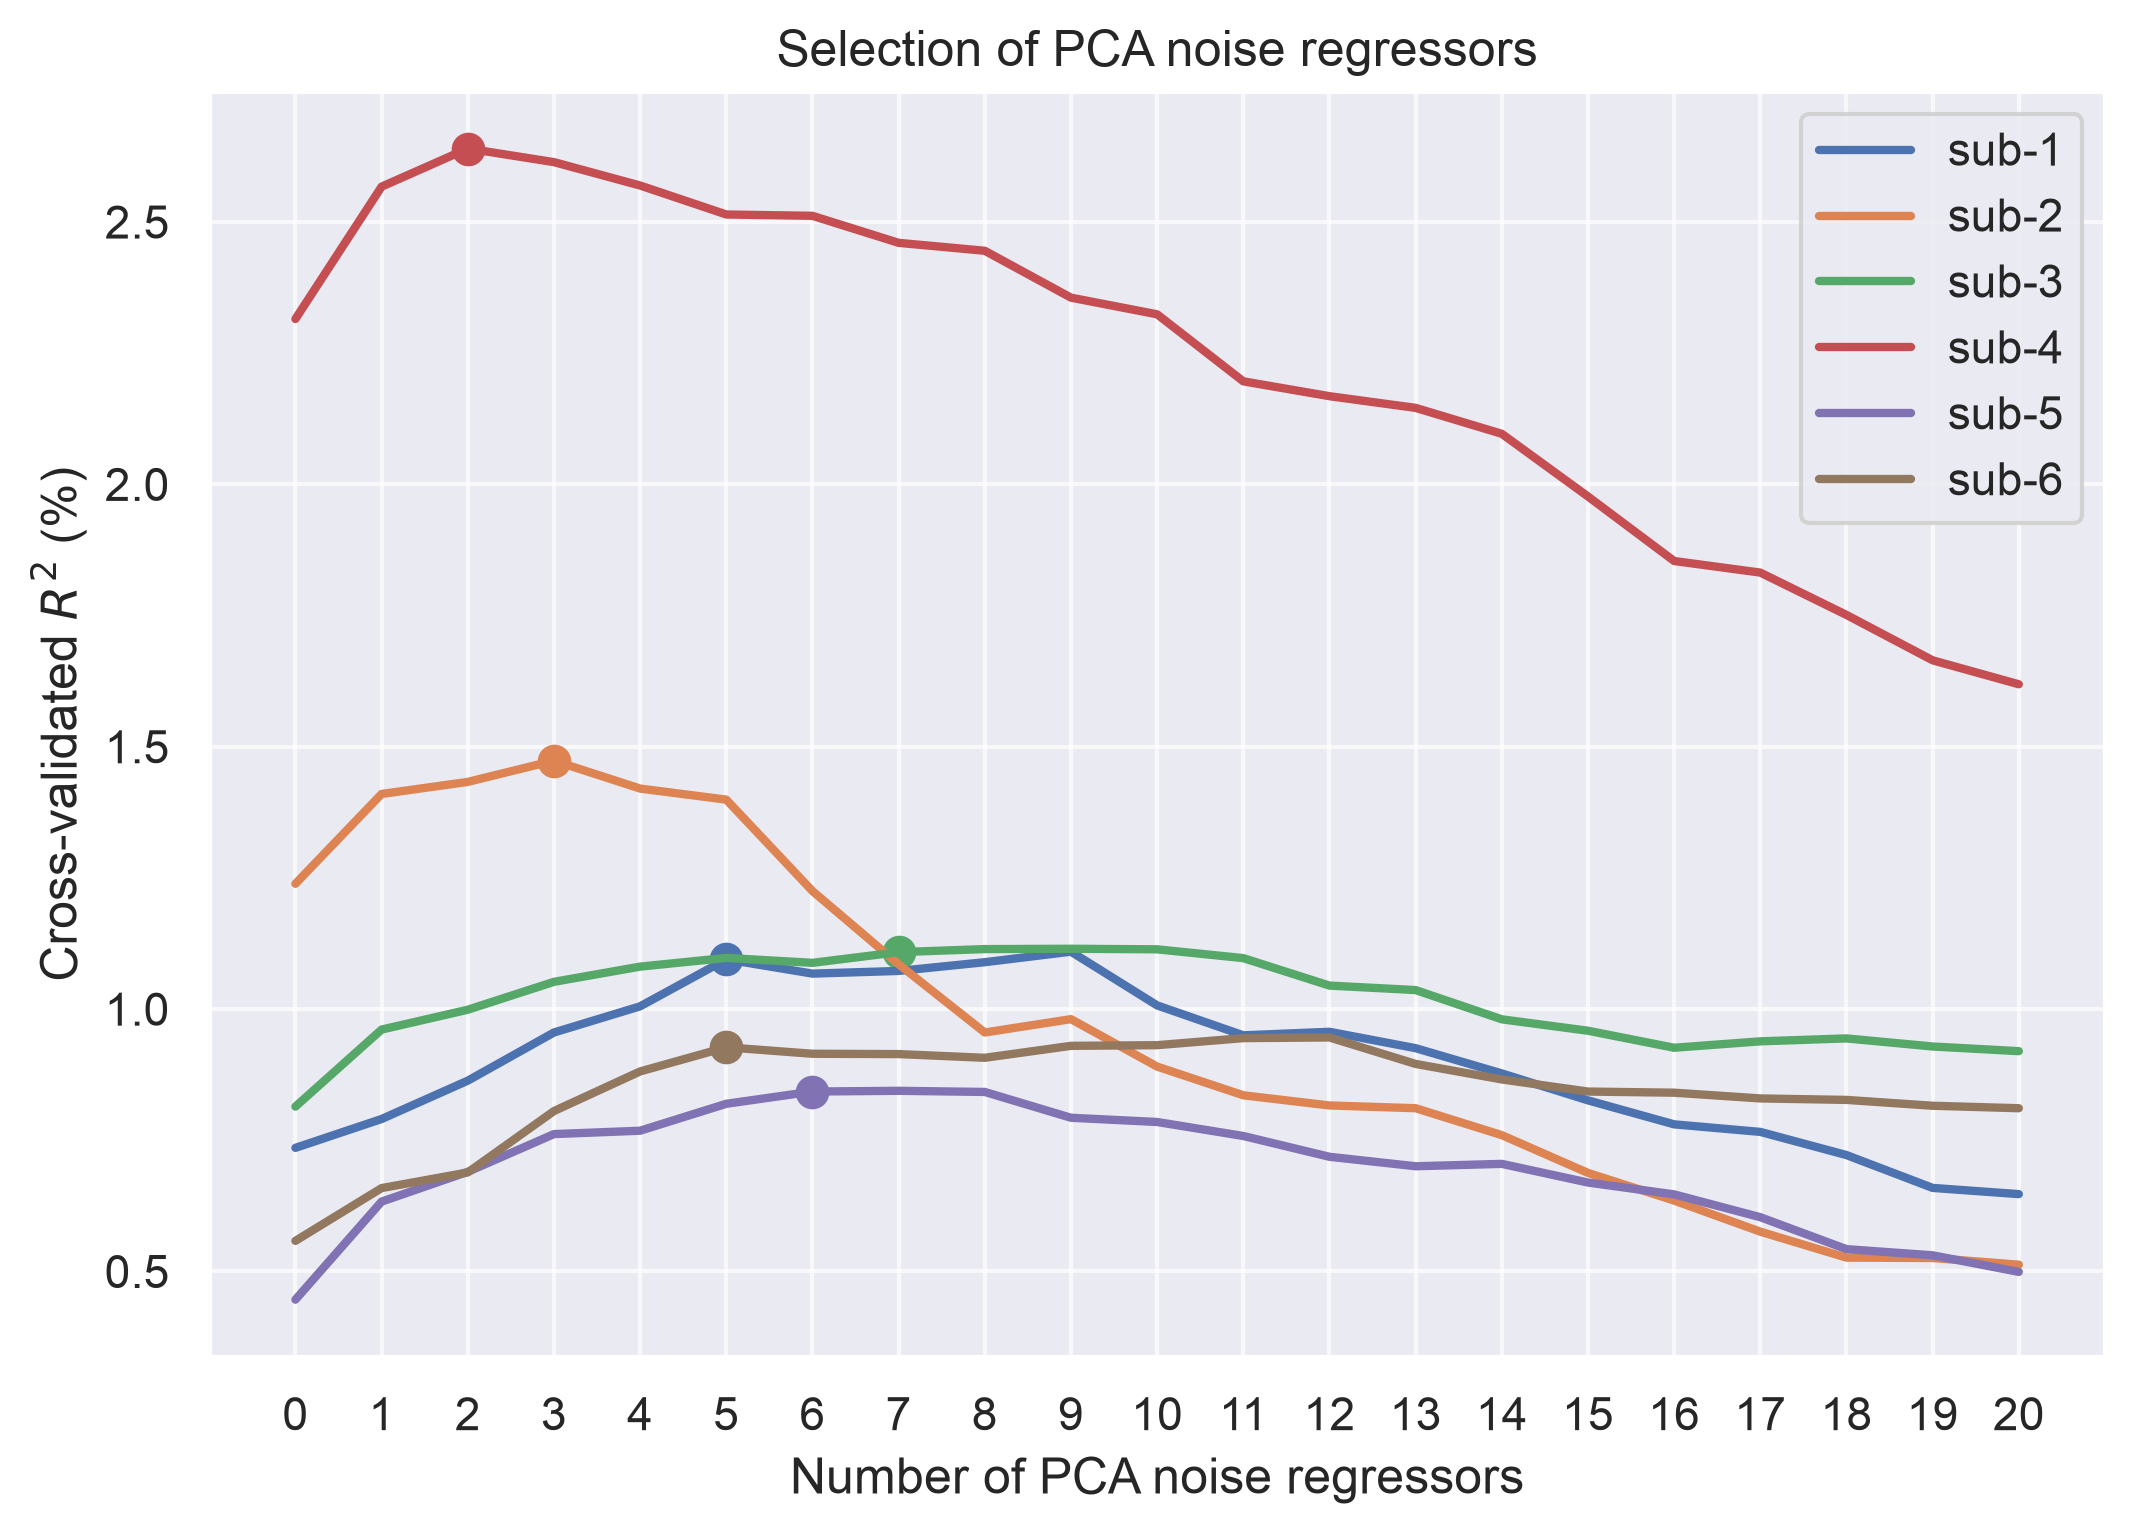
\includegraphics[width=\textwidth]{fig/pca_component_comparison.png}
    \caption{Prediction accuracy as a function of the number of PCA noise regressors with the chosen final number of components for each subject in PCA-assisted GLM denoising.}
    \label{fig:pca-components}
\end{figure}

Figure~\ref{fig:pca-components} shows plots of prediction accuracy values for each of the number of PCA noise regressors for each subject. Additionally, the dots indicate the final number of PCA noise regressors selected using the $95\%$ of maximum improvement criterion described in Section~\ref{section:pca-regressors}. This figure mirrors \cite[Figure 2C]{glm-denoise}.

The performance curves generally increase initially, reach a maximum, and subsequently decrease as additional PCA noise regressors are introduced. A particularly pronounced pattern can be observed for subject 4, which also obtains the highest cross-validated $R^2$ values, and for subject 2, whose prediction accuracy decreases relatively rapidly after approximately three to five components. The curves for the remaining subjects are flatter, although a similar tendency can still be observed. These results also indicate that setting the maximum number of candidate noise regressors to $k_{\max}=20$ was sufficient, since the selected numbers occur well below this boundary and the cross-validated $R^2$ generally decreases for larger numbers of regressors.

The chosen number of components is in the range $[2, 7]$, never reaching a double-digit number. The numbers vary between subjects, supporting the use of data-driven component selection rather than a single fixed number of nuisance regressors for all participants. For every subject, the selected number of PCA noise regressors is greater than zero. Selecting zero PCA noise regressors would reduce the procedure to the standard GLM. As a result, the added noise regressors seem to show an improvement in overall model prediction accuracy, although a relatively small one. These results are discussed further in Section~\ref{section:results-remarks}.

\subsection{ICA-based denoising components}

\begin{figure}[!htbp]
    \centering
    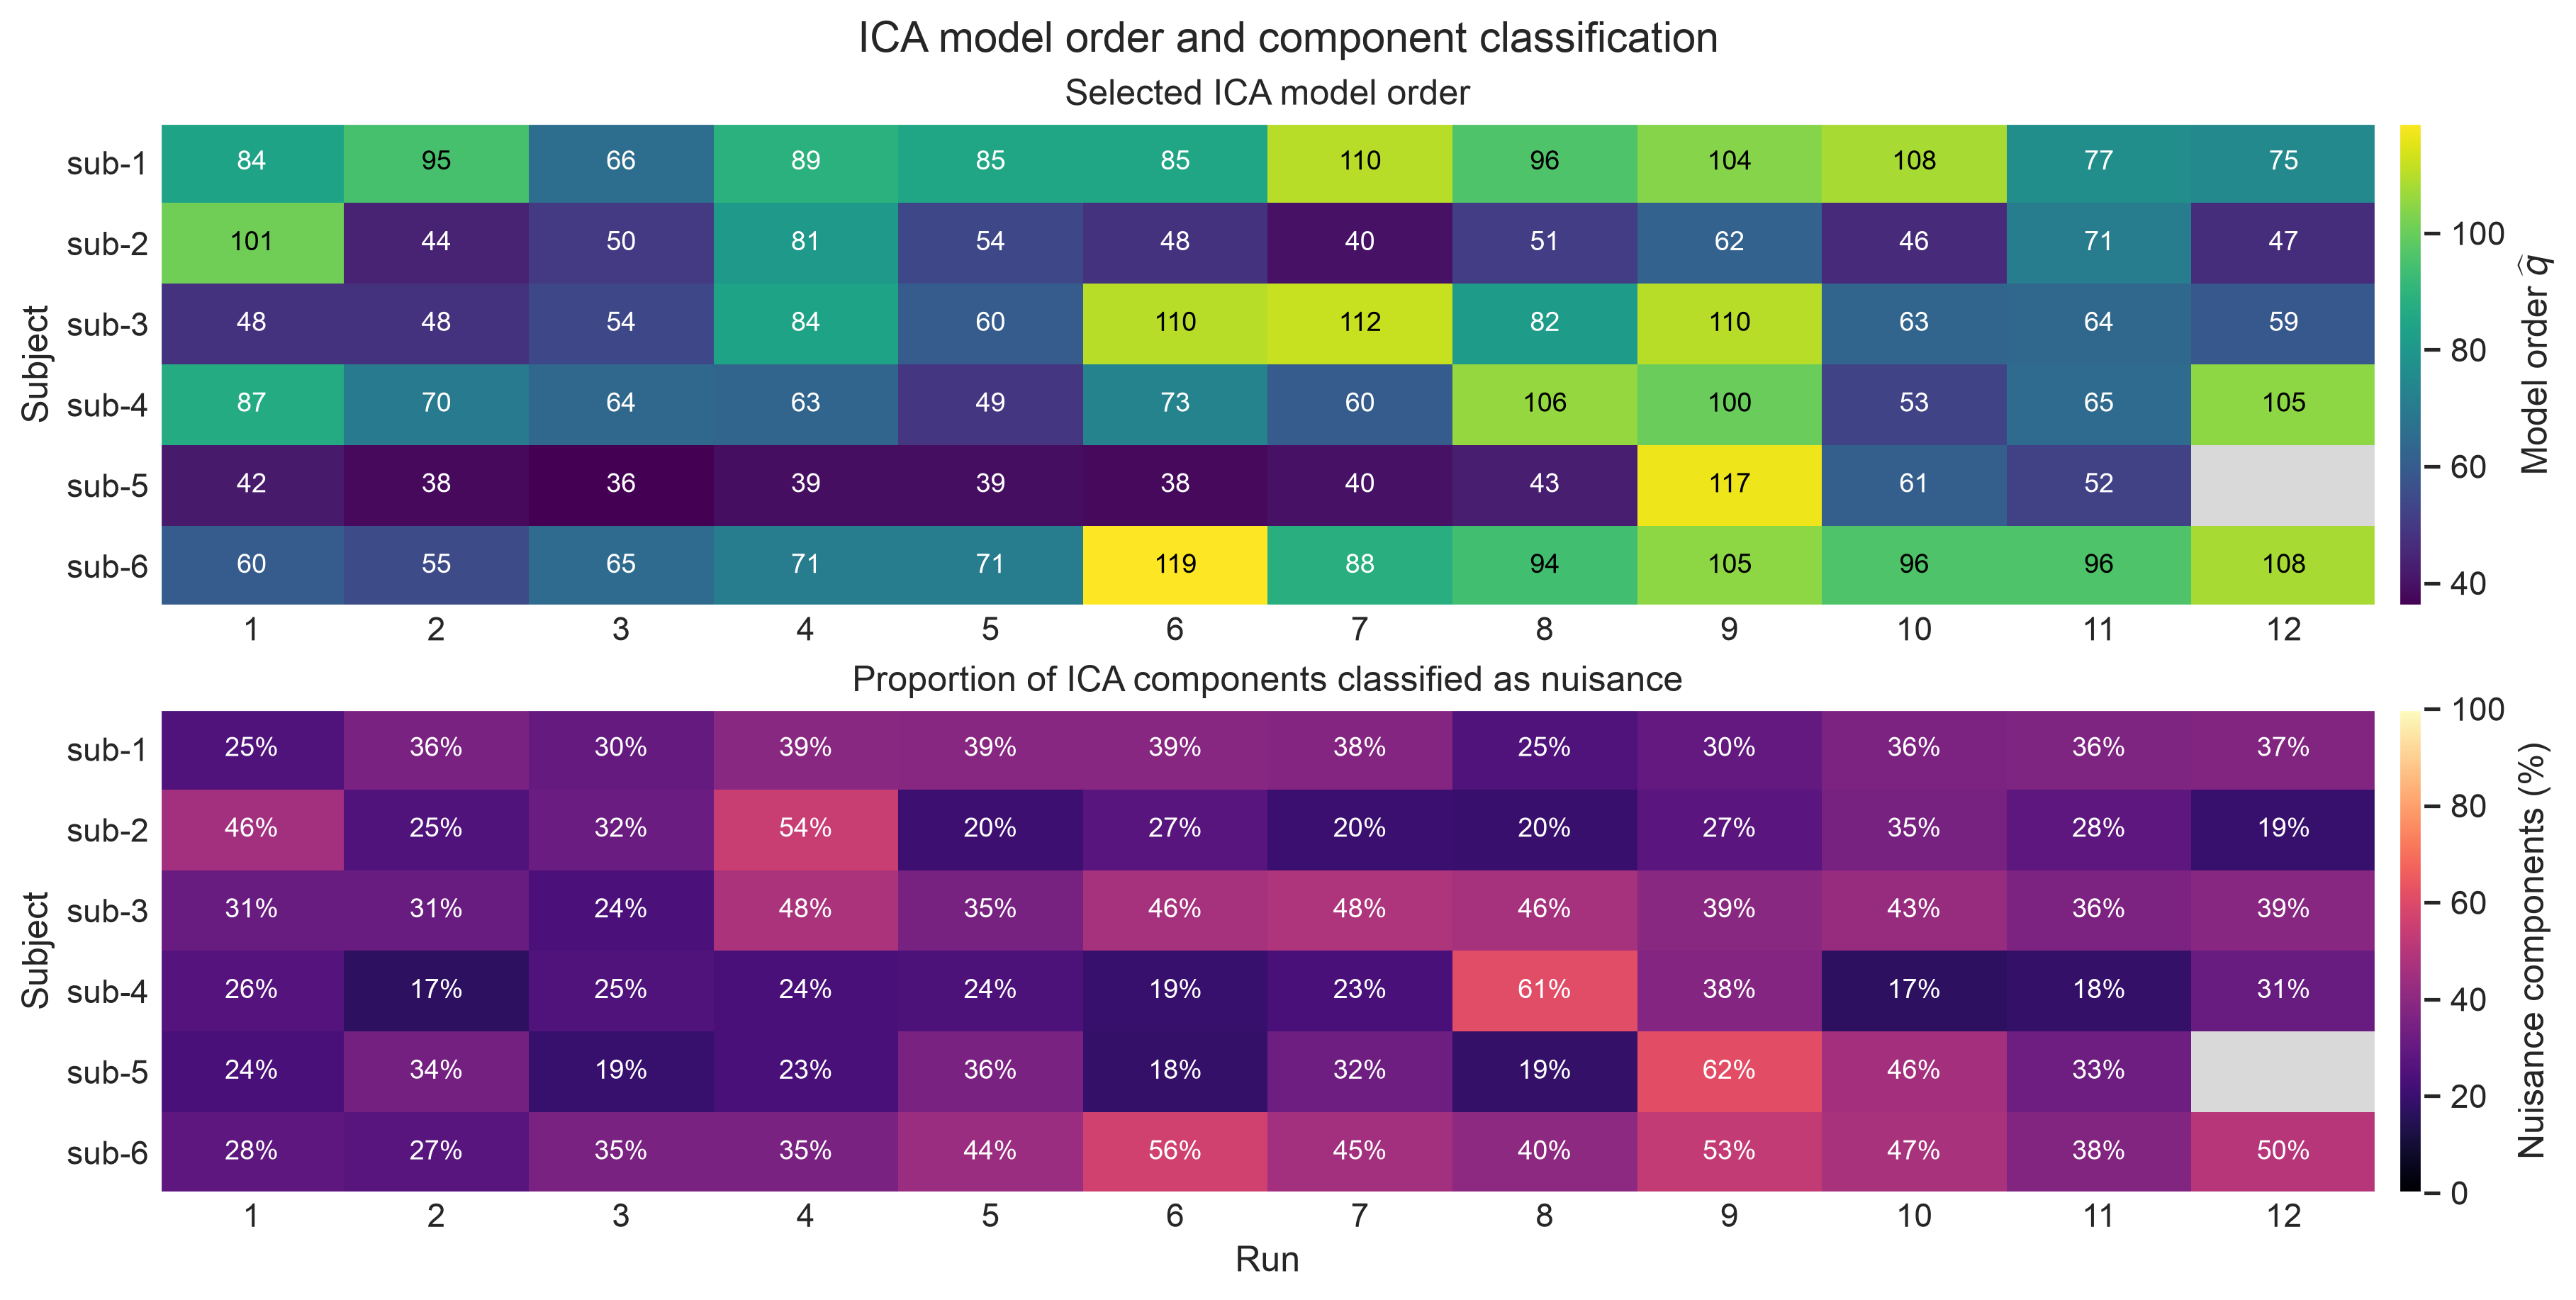
\includegraphics[width=\textwidth]{fig/ica_component_comparison.png}
    \caption{Two heatmaps representing the selected model order $\widehat{q}$ and the proportion of ICA components classified as nuisance, respectively.}
    \label{fig:ica-components}
\end{figure}

After selecting the model order and estimating the independent components, the criterion presented in Equation~\eqref{eq:classification-criterion} classifies each component as either task-related or nuisance. If $z_j > c$, component $j$ is classified as task-related; otherwise, it is classified as nuisance. Figure~\ref{fig:ica-components} presents two heatmaps. The upper heatmap shows the selected model order $\widehat{q}$, i.e., the number of dimensions retained prior to ICA estimation. The lower heatmap presents the proportion of the resulting ICA components classified as nuisance. This proportion and the resulting task-related component classification proportion can be expressed as 

\begin{equation}
    \pi_{\mathrm{nuis}} = \frac{n_{\mathrm{nuis}}}{\widehat{q}}, \qquad 
    \pi_{\mathrm{task}} = \frac{n_{\mathrm{task}}}{\widehat{q}} = 1 - \frac{n_{\mathrm{nuis}}}{\widehat{q}}, \qquad
    \pi_{\mathrm{task}}+\pi_{\mathrm{nuis}}=1.
\end{equation}

The selected model order $\widehat{q}$ varies considerably both between subjects and between runs. The smallest value is $\widehat{q}=36$, obtained for subject 5 in run 3, whereas the largest is $\widehat{q}=119$, obtained for subject 6 in run 6. No clear common pattern across subjects is apparent. Subject 5 is a notable exception, with model orders mostly concentrated in the range $[36,61]$, apart from run 9, for which $\widehat{q}=117$.

The proportion of ICA components classified as nuisance ranges approximately from $17\%$ to $62\%$, with most values remaining below $50\%$. Similarly to the selected model order, the nuisance-component proportion varies considerably across runs and subjects. No clear monotonic relationship between the selected model order and the proportion of components classified as nuisance is apparent from the heatmaps.

The substantial run-to-run variability in both the selected model order and the nuisance-component proportion, together with the poor prediction accuracy of ICA-based denoising presented in Section~\ref{section:prediction-results}, motivates a closer examination of the component-classification criterion.

To examine the classification criterion more closely, Figure~\ref{fig:ica-z-scores} presents the task-association $z$-scores for individual ICA components across runs and subjects. The dashed line indicates the classification threshold $c=0$ adopted from \cite{glm-denoise}, while the shaded region indicates scores classified as nuisance. A substantial concentration of component scores can be observed around the classification boundary. In particular, many components have slightly negative $z$-scores and are therefore classified as nuisance, despite lying close to the threshold. Moreover, the distribution does not exhibit an obvious separation into two distinct groups corresponding to task-related and nuisance components. This suggests that the binary classification may be sensitive to relatively small differences in the task-association score.

These results suggest that the task-association $z$-score and the fixed threshold $c=0$ may not provide a sufficiently discriminative criterion for component classification in the analyzed dataset. Components with scores close to zero are assigned to one of the two groups, although the score distributions do not show a clear boundary between them. Consequently, components containing useful task-related information may potentially be classified as nuisance and removed during denoising. Such removal could reduce prediction accuracy by subtracting signal components that contribute to the task-related response.

Moreover, the characteristics of the analyzed dataset may further affect the performance of ICA-based denoising. These limitations and possible explanations are discussed in Section~\ref{section:results-remarks}.

\begin{figure}[!htbp]
    \centering
    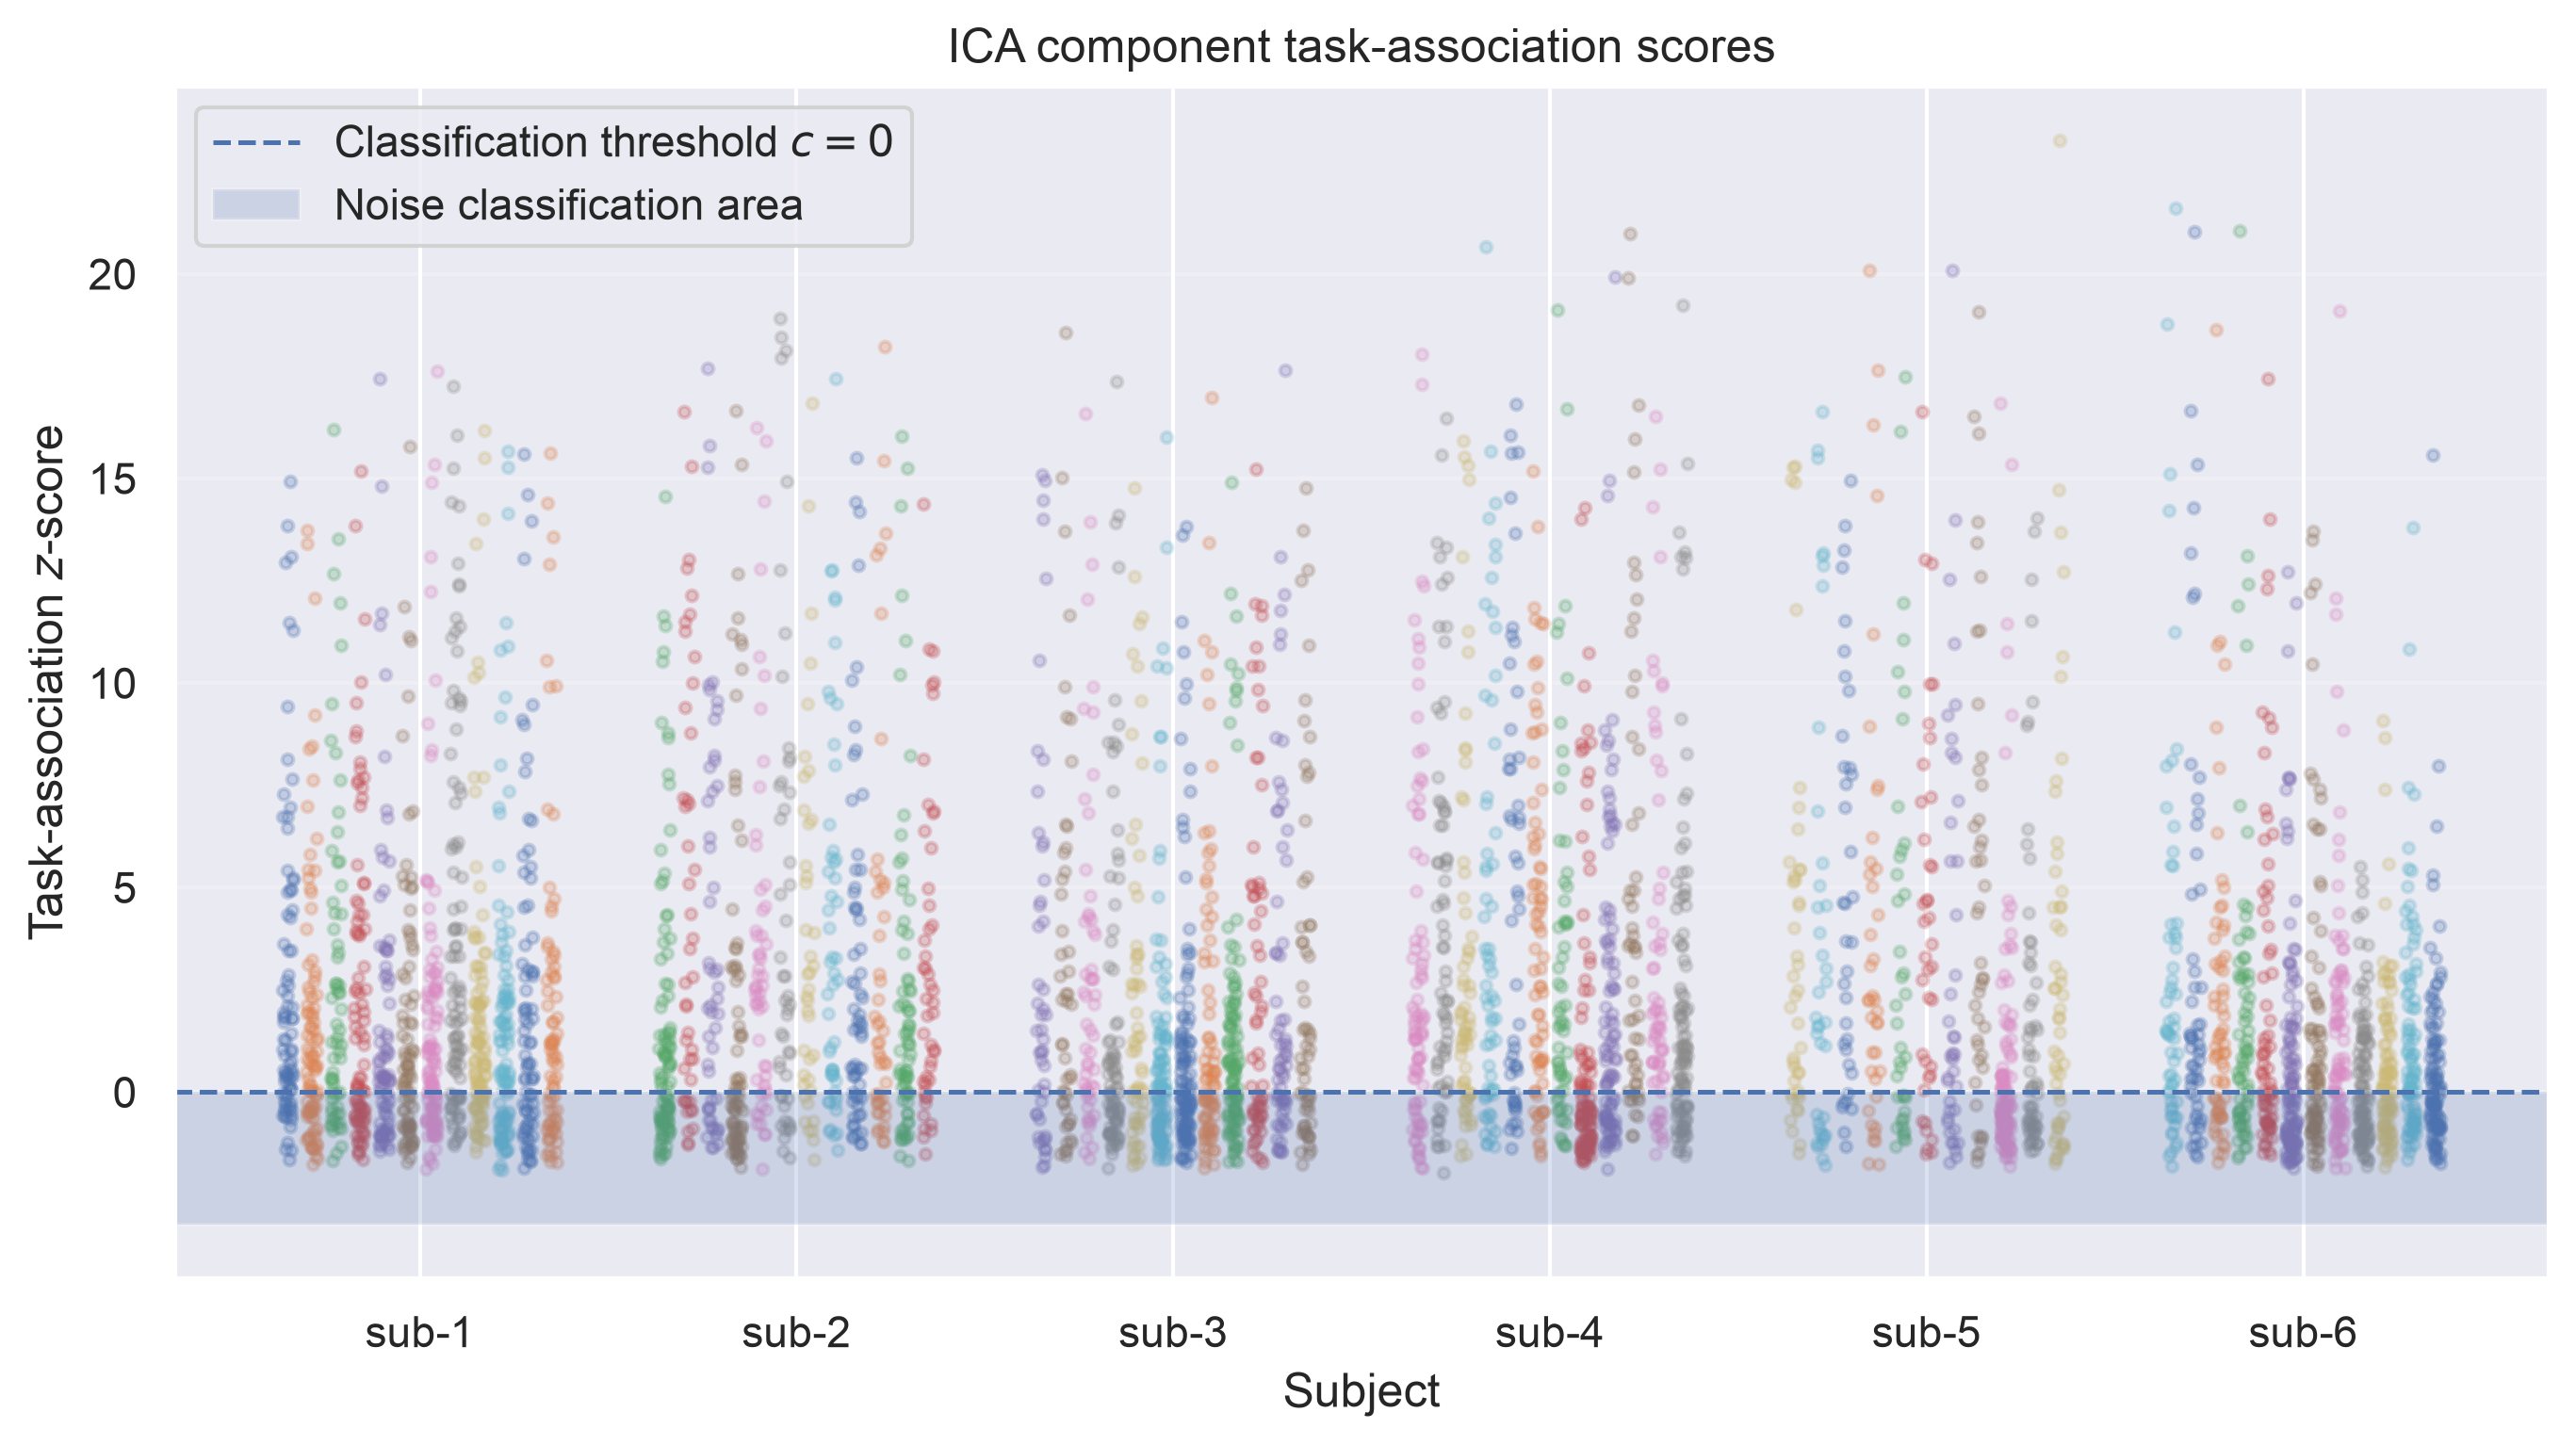
\includegraphics[width=\textwidth]{fig/ica_z_scores_comparison.png}
    \caption{Task-association $z$-scores of ICA components across runs and subjects, with the classification threshold $c=0$ and the region corresponding to nuisance-component classification.}
    \label{fig:ica-z-scores}
\end{figure}

\newpage
\section{Task-related coefficients stability analysis}

\begin{figure}[!htbp]
    \centering
    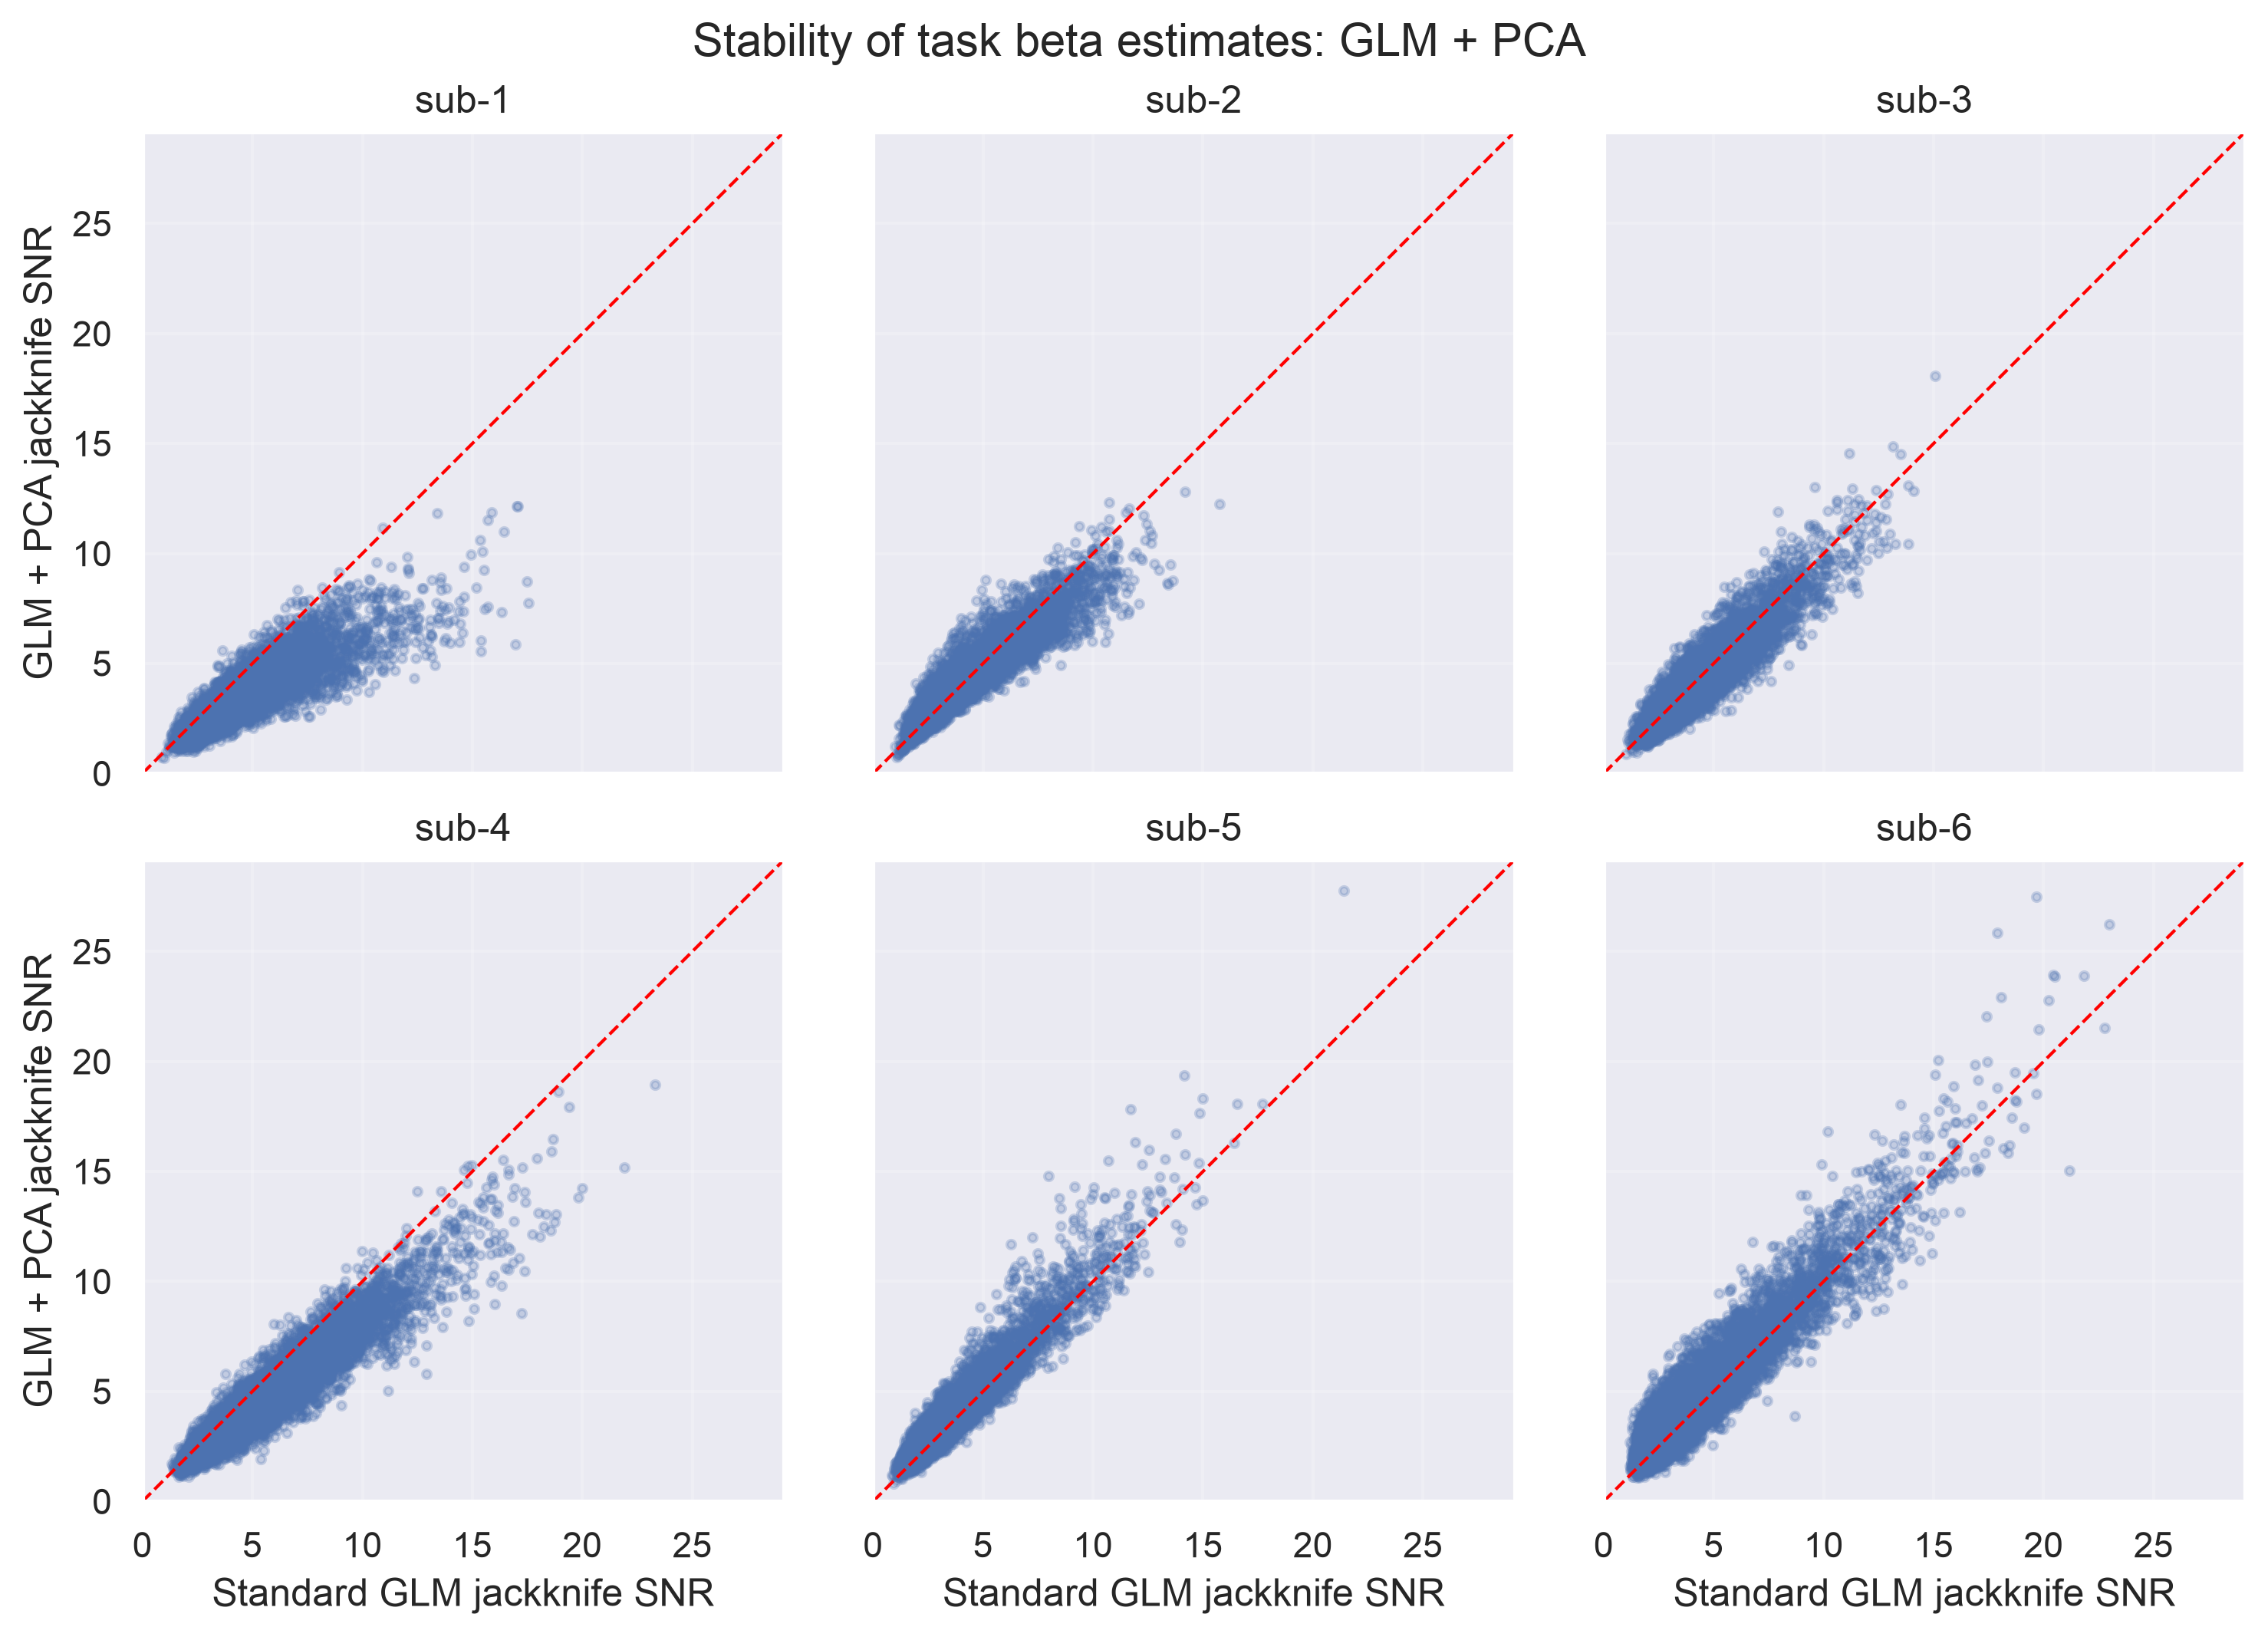
\includegraphics[scale=0.5]{fig/snr_scatter_glm_pca.png}
    \caption{Scatter plots comparing voxelwise jackknife SNR of task-related coefficient estimates obtained with PCA-assisted GLM denoising and the standard GLM for each subject.}
    \label{fig:snr-glm-pca}
\end{figure}
\begin{figure}[!htbp]
    \centering
    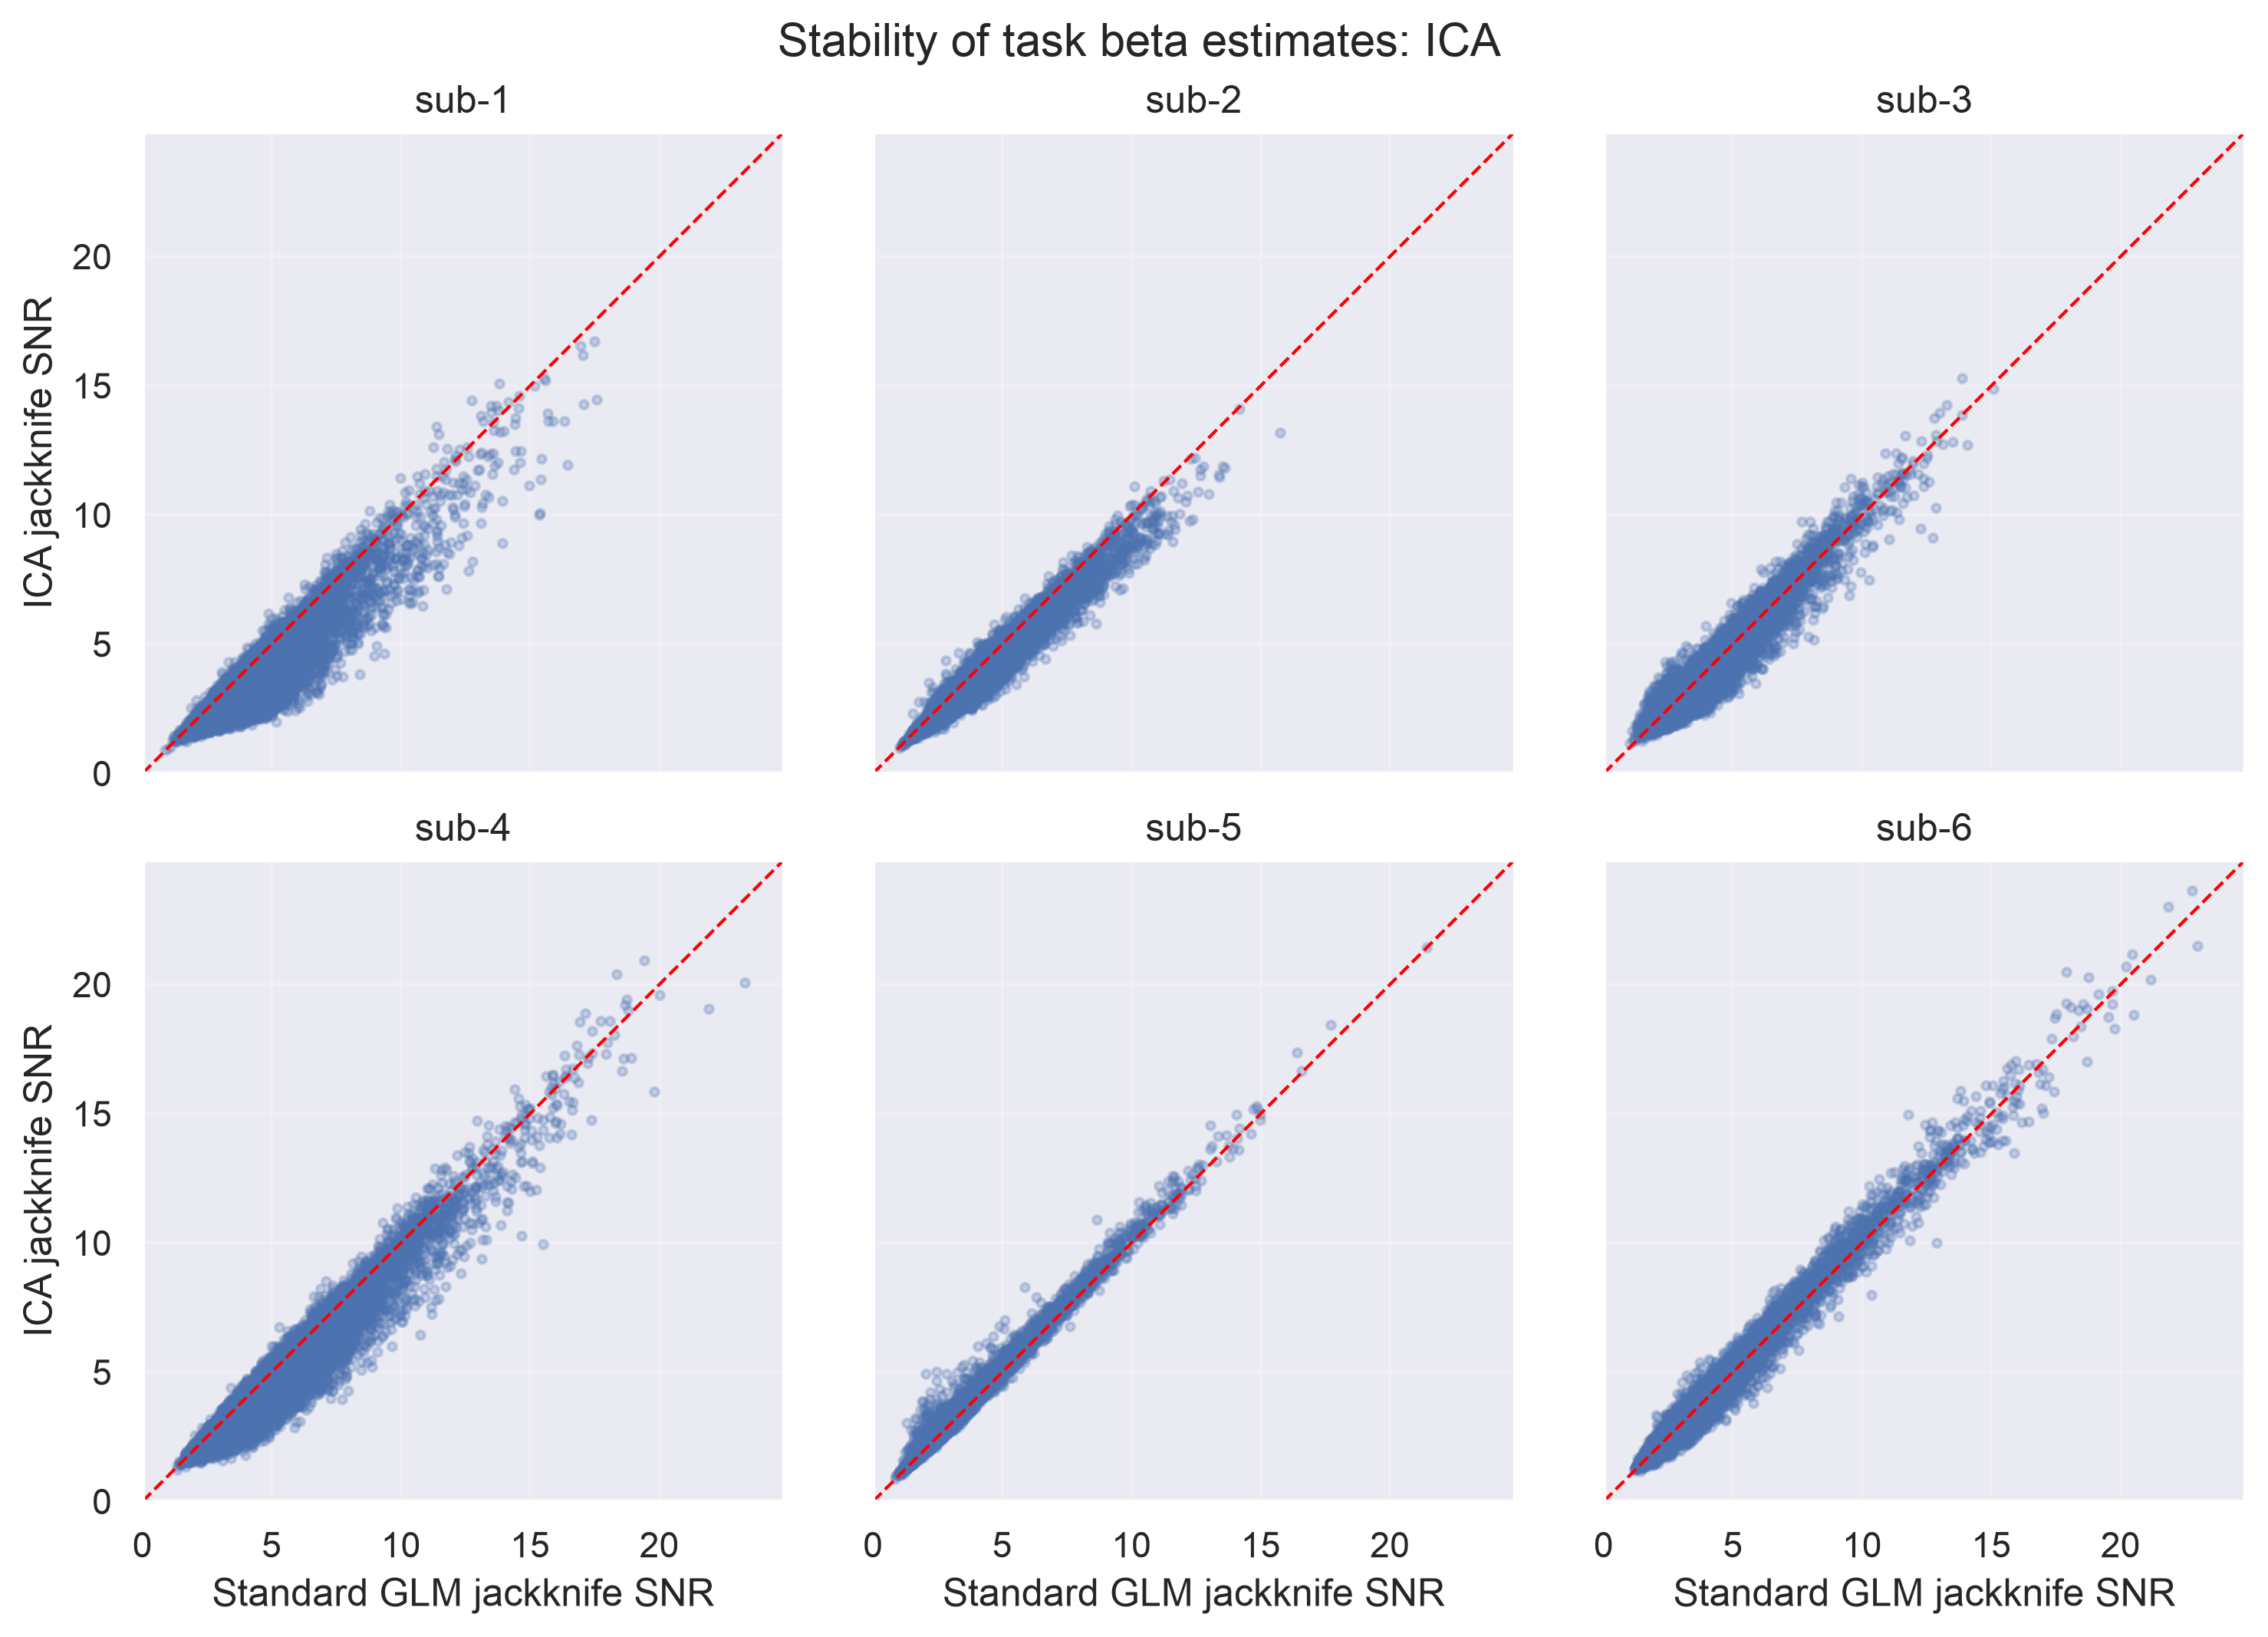
\includegraphics[scale=0.5]{fig/snr_scatter_ica.png}
    \caption{Scatter plots comparing voxelwise jackknife SNR of task-related coefficient estimates obtained with ICA-based denoising and the standard GLM for each subject.}
    \label{fig:snr-ica}
\end{figure}

Figures~\ref{fig:snr-glm-pca}~and~\ref{fig:snr-ica} compare the jackknife signal-to-noise ratio of voxelwise task-related coefficient estimates presented in Equation~\eqref{eq:jackknife-snr}. All values were obtained with PCA-assisted GLM and ICA-based denoising, respectively, against the standard GLM. For each point, corresponding to a voxel from the common evaluation voxel set, the $x$-coordinate represents the SNR obtained with the standard GLM, while the $y$-coordinate represents the SNR obtained with the analyzed denoising method. Because the numerator of the metric described in Equation~\eqref{eq:jackknife-snr} is shared across methods for a given voxel, differences in SNR arise from differences in the jackknife standard error. Therefore, the comparison primarily reflects differences in the stability of the estimated task-related coefficients rather than differences in their magnitude.

The identity line $y=x$ represents equal jackknife SNR for the two compared methods. Since the signal term is shared, a point above this line corresponds to a smaller jackknife standard error and therefore a more stable task-related coefficient estimate for the denoising method. Conversely, a point below the line indicates greater jackknife variability relative to the standard GLM. These figures are analogous to the SNR comparison presented in \mbox{\cite[Figure 4C]{glm-denoise}}.

For PCA-assisted GLM denoising, shown in Figure~\ref{fig:snr-glm-pca}, the voxel clouds for subjects 1, 2, and 4 are predominantly located below the identity line. The difference becomes particularly visible for voxels with moderate and high standard GLM SNR, indicating that the PCA-assisted estimates tend to have greater jackknife variability for these subjects. Subject 3 exhibits a weaker displacement, with the voxel cloud remaining closer to the identity line. For subjects 5 and 6, the points are also distributed more closely around the identity line, with a portion of the voxels lying above it. Subject 6 in particular shows positive deviations for some voxels with larger standard GLM SNR. Overall, however, no consistent upward displacement is observed across all subjects.

\newpage
These results indicate that the small improvement in prediction accuracy obtained with PCA-assisted GLM denoising does not translate directly into improved stability of the task-related coefficient estimates. This contrasts with the results reported for the original GLMdenoise method in \cite{glm-denoise}, where an overall increase in beta-weight SNR relative to the standard GLM was observed.

This result can be compared with the prediction accuracy analysis presented in Section~\ref{section:prediction-results}. PCA-assisted GLM denoising produced a small positive improvement in outer-CV $R^2$, while its task-related coefficient estimates are not consistently more stable than those obtained with the standard GLM. The two results are not contradictory, since outer-CV $R^2$ measures predictive generalization to left-out data, whereas jackknife SNR quantifies the stability of coefficient estimates across training sets. One possible explanation is that the additional data-driven model-selection procedure provides a small predictive benefit while simultaneously making the resulting estimates more sensitive to the particular set of runs used for training.

The ICA-based results in Figure~\ref{fig:snr-ica} are broadly consistent with the previous prediction accuracy analysis. Subjects 1, 2, and 4 exhibit a clear downward displacement relative to the identity line, indicating lower stability of the task-related coefficient estimates than for the standard GLM. The effect is most pronounced for subject 1, particularly for voxels with moderate and high standard GLM SNR. Subject 3 also exhibits a tendency towards lower ICA SNR, although the difference is less pronounced. In contrast, subjects 5 and 6 show voxel clouds located considerably closer to the identity line, indicating smaller differences in coefficient stability between ICA-based denoising and the standard GLM.

The subject-specific pattern is similar to that observed for outer-CV prediction accuracy. Subjects for which ICA-based denoising produced the strongest deterioration in prediction accuracy also tend to exhibit lower jackknife SNR, whereas subjects 5 and 6 show relatively small differences from the standard GLM under both evaluation criteria. This suggests that the poorer ICA results are not restricted to the prediction-accuracy metric, but are also reflected in the stability of the estimated task-related coefficients.

Another visible feature of both figures is that the absolute differences between methods become more apparent for voxels with larger standard GLM SNR. Near the origin, all methods produce low SNR values and the voxel clouds are tightly concentrated. At larger SNR values, deviations from the identity line become easier to distinguish.

From the perspective of denoising, this behavior is generally undesirable. A successful nuisance-removal procedure would ideally preserve or improve the stability of task-related coefficient estimates. Instead, PCA-assisted GLM denoising provides no consistent stability improvement despite its small gain in prediction accuracy, while ICA-based denoising reduces both prediction accuracy and coefficient stability for several subjects. The standard GLM therefore remains a strong reference method also with respect to the reliability of the estimated task-related coefficients.

\section{Beta maps analysis}

Beta maps can be produced separately for each subject and stimulus category. Presenting all possible combinations would result in a large number of figures. Therefore, a single representative subject and a single stimulus category were selected for the spatial analysis.

The subject was selected based on the similarity of its method-specific median outer-CV $R^2$ values to the corresponding across-subject median values. According to the prediction accuracy results presented in Figure~\ref{fig:median-r2}, subject 3 provides a representative performance profile, with the median $R^2$ values obtained for the standard GLM, PCA-assisted GLM denoising, and ICA-based denoising all remaining close to the central tendency observed across subjects.

The stimulus category was selected with reference to the original analysis of the dataset presented in \cite{dataset-cit1}. Although several visual categories are considered, faces and houses constitute one of the principal category comparisons discussed by the authors. Therefore, the face category was selected for the beta-map analysis, while the subsequent contrast analysis considers the face-versus-house contrast.

\begin{figure}[!htbp]
    \centering
    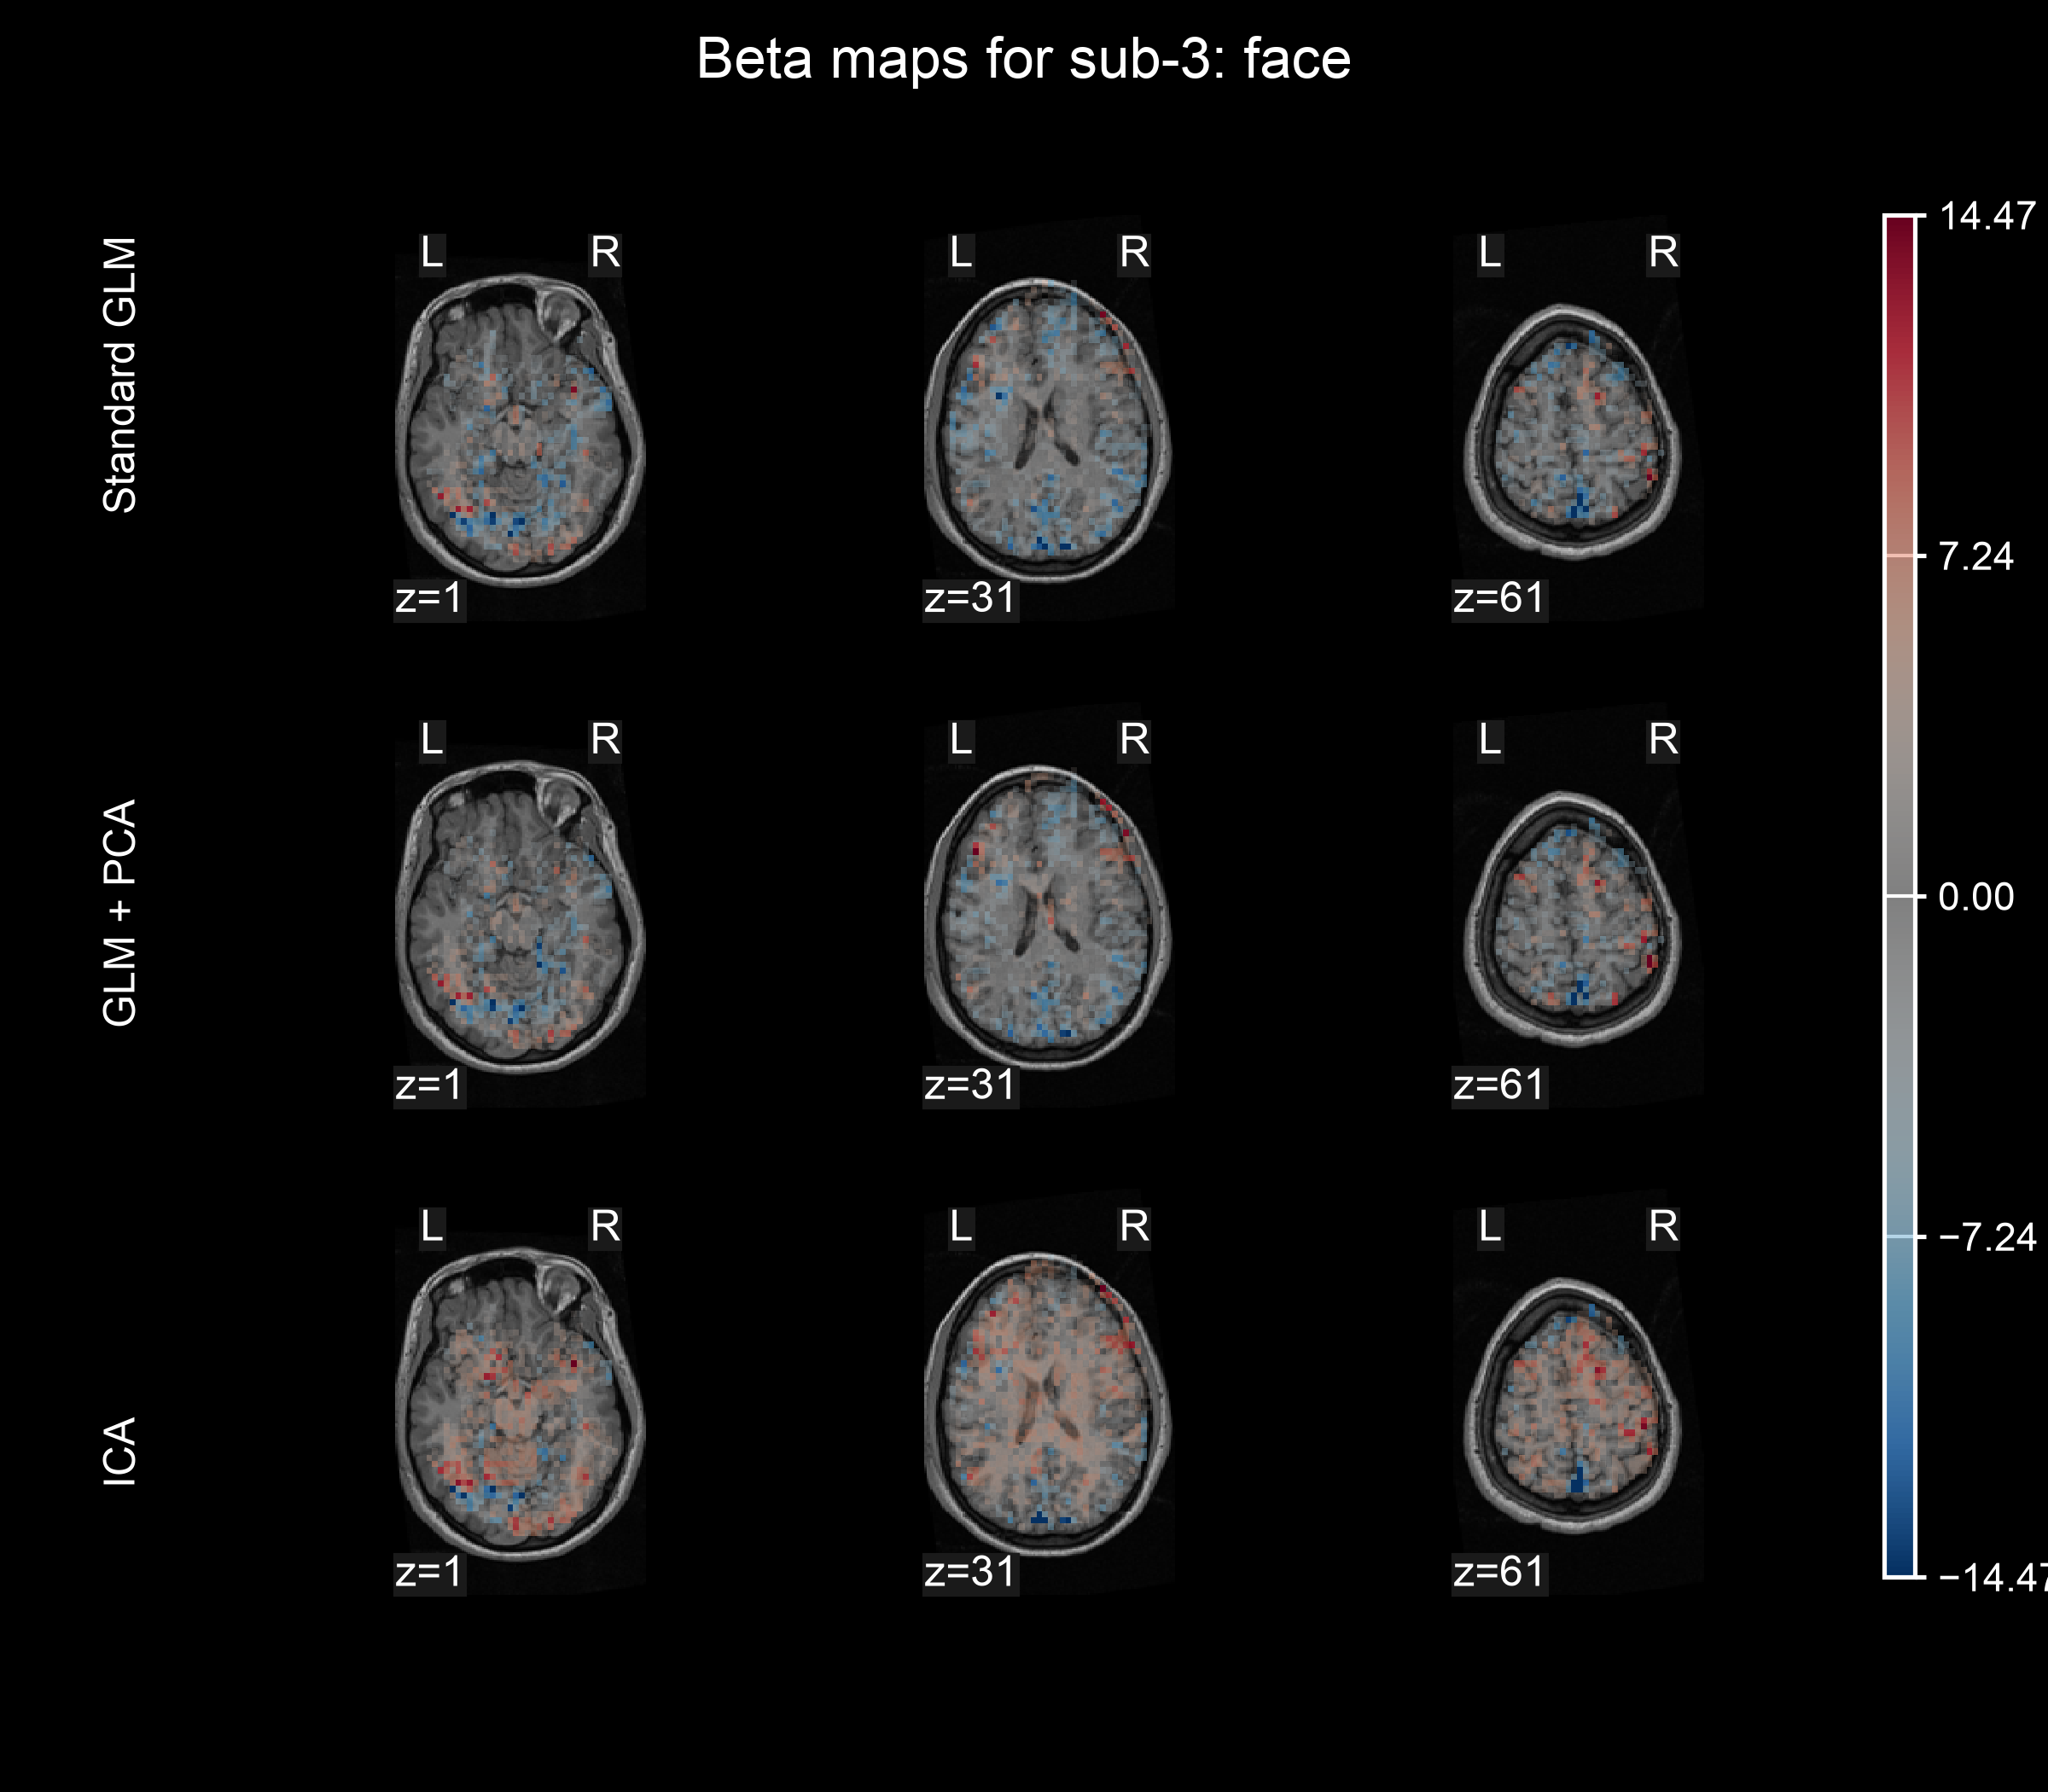
\includegraphics[scale=0.5]{fig/sub-3_beta_face.png}
    \caption{$z$-axis slices of the face-category beta estimates for subject 3 obtained with the standard GLM, PCA-assisted GLM denoising, and ICA-based denoising, shown using a common color scale over the T1-weighted anatomical image.}
    \label{fig:beta-maps}
\end{figure}

Figure~\ref{fig:beta-maps} presents the face-category beta maps for subject 3. Each row corresponds to one of the analyzed methods and contains three slices at the same $z$-coordinates, allowing direct spatial comparison between methods. A symmetric color scale shared across all methods represents the sign and magnitude of the estimated coefficients. Positive and negative colors correspond to positive and negative face-regressor coefficients, respectively. Values close to zero are displayed with reduced opacity, allowing the underlying T1-weighted anatomical image to remain visible. No statistical threshold is applied to the beta estimates.

The standard GLM and PCA-assisted GLM maps are spatially similar. Across the displayed slices, regions with positive and negative coefficients generally occur in similar locations across the presented slices. PCA changes the magnitude of some local coefficient estimates but largely preserves the spatial structure observed for the standard GLM. This is consistent with the preceding prediction-accuracy and task-related coefficient-stability analyses, where PCA-assisted denoising produced only modest changes relative to the standard GLM.

\newpage
ICA-based denoising produces more visible differences. Its maps contain more spatially spread positive estimates across all three slices, particularly at $z=1$. The positive coefficient estimates are also more spatially spread at intermediate magnitudes, visible as broader orange regions in the displayed maps. Simultaneously, regions containing larger-magnitude positive and negative coefficients remain broadly recognizable relative to the GLM-based methods. Nevertheless, the overall spatial pattern departs more strongly from the GLM-based denoising methods. This greater departure from the standard GLM is consistent with the poorer outer-CV prediction accuracy and lower jackknife stability previously observed for subject 3.

Overall, PCA-assisted GLM denoising largely preserves the spatial organization of the standard GLM beta estimates, whereas ICA-based denoising produces larger changes in their magnitude and spatial distribution.

\section{Contrast \texorpdfstring{$t$}{t}-maps analysis}

As mentioned in the preceding section, subject 3 is selected for the spatial analysis. The analyzed contrast is $\text{face} > \text{house}$. The resulting contrast $t$-maps are presented in Figure~\ref{fig:t-maps}. As in the beta-map comparison, each row corresponds to one of the analyzed methods and contains the same axial slices as Figure~\ref{fig:beta-maps}. A symmetric color scale shared across all methods represents the sign and magnitude of the $t$-statistic. For visualization, values with $|t| < 3$ are not displayed, contrasting the thresholding in \cite[Figure 5]{glm-denoise}, which displays only $t > 3$. The statistical maps are overlaid on the corresponding T1-weighted anatomical image.

\begin{figure}[!htbp]
    \centering
    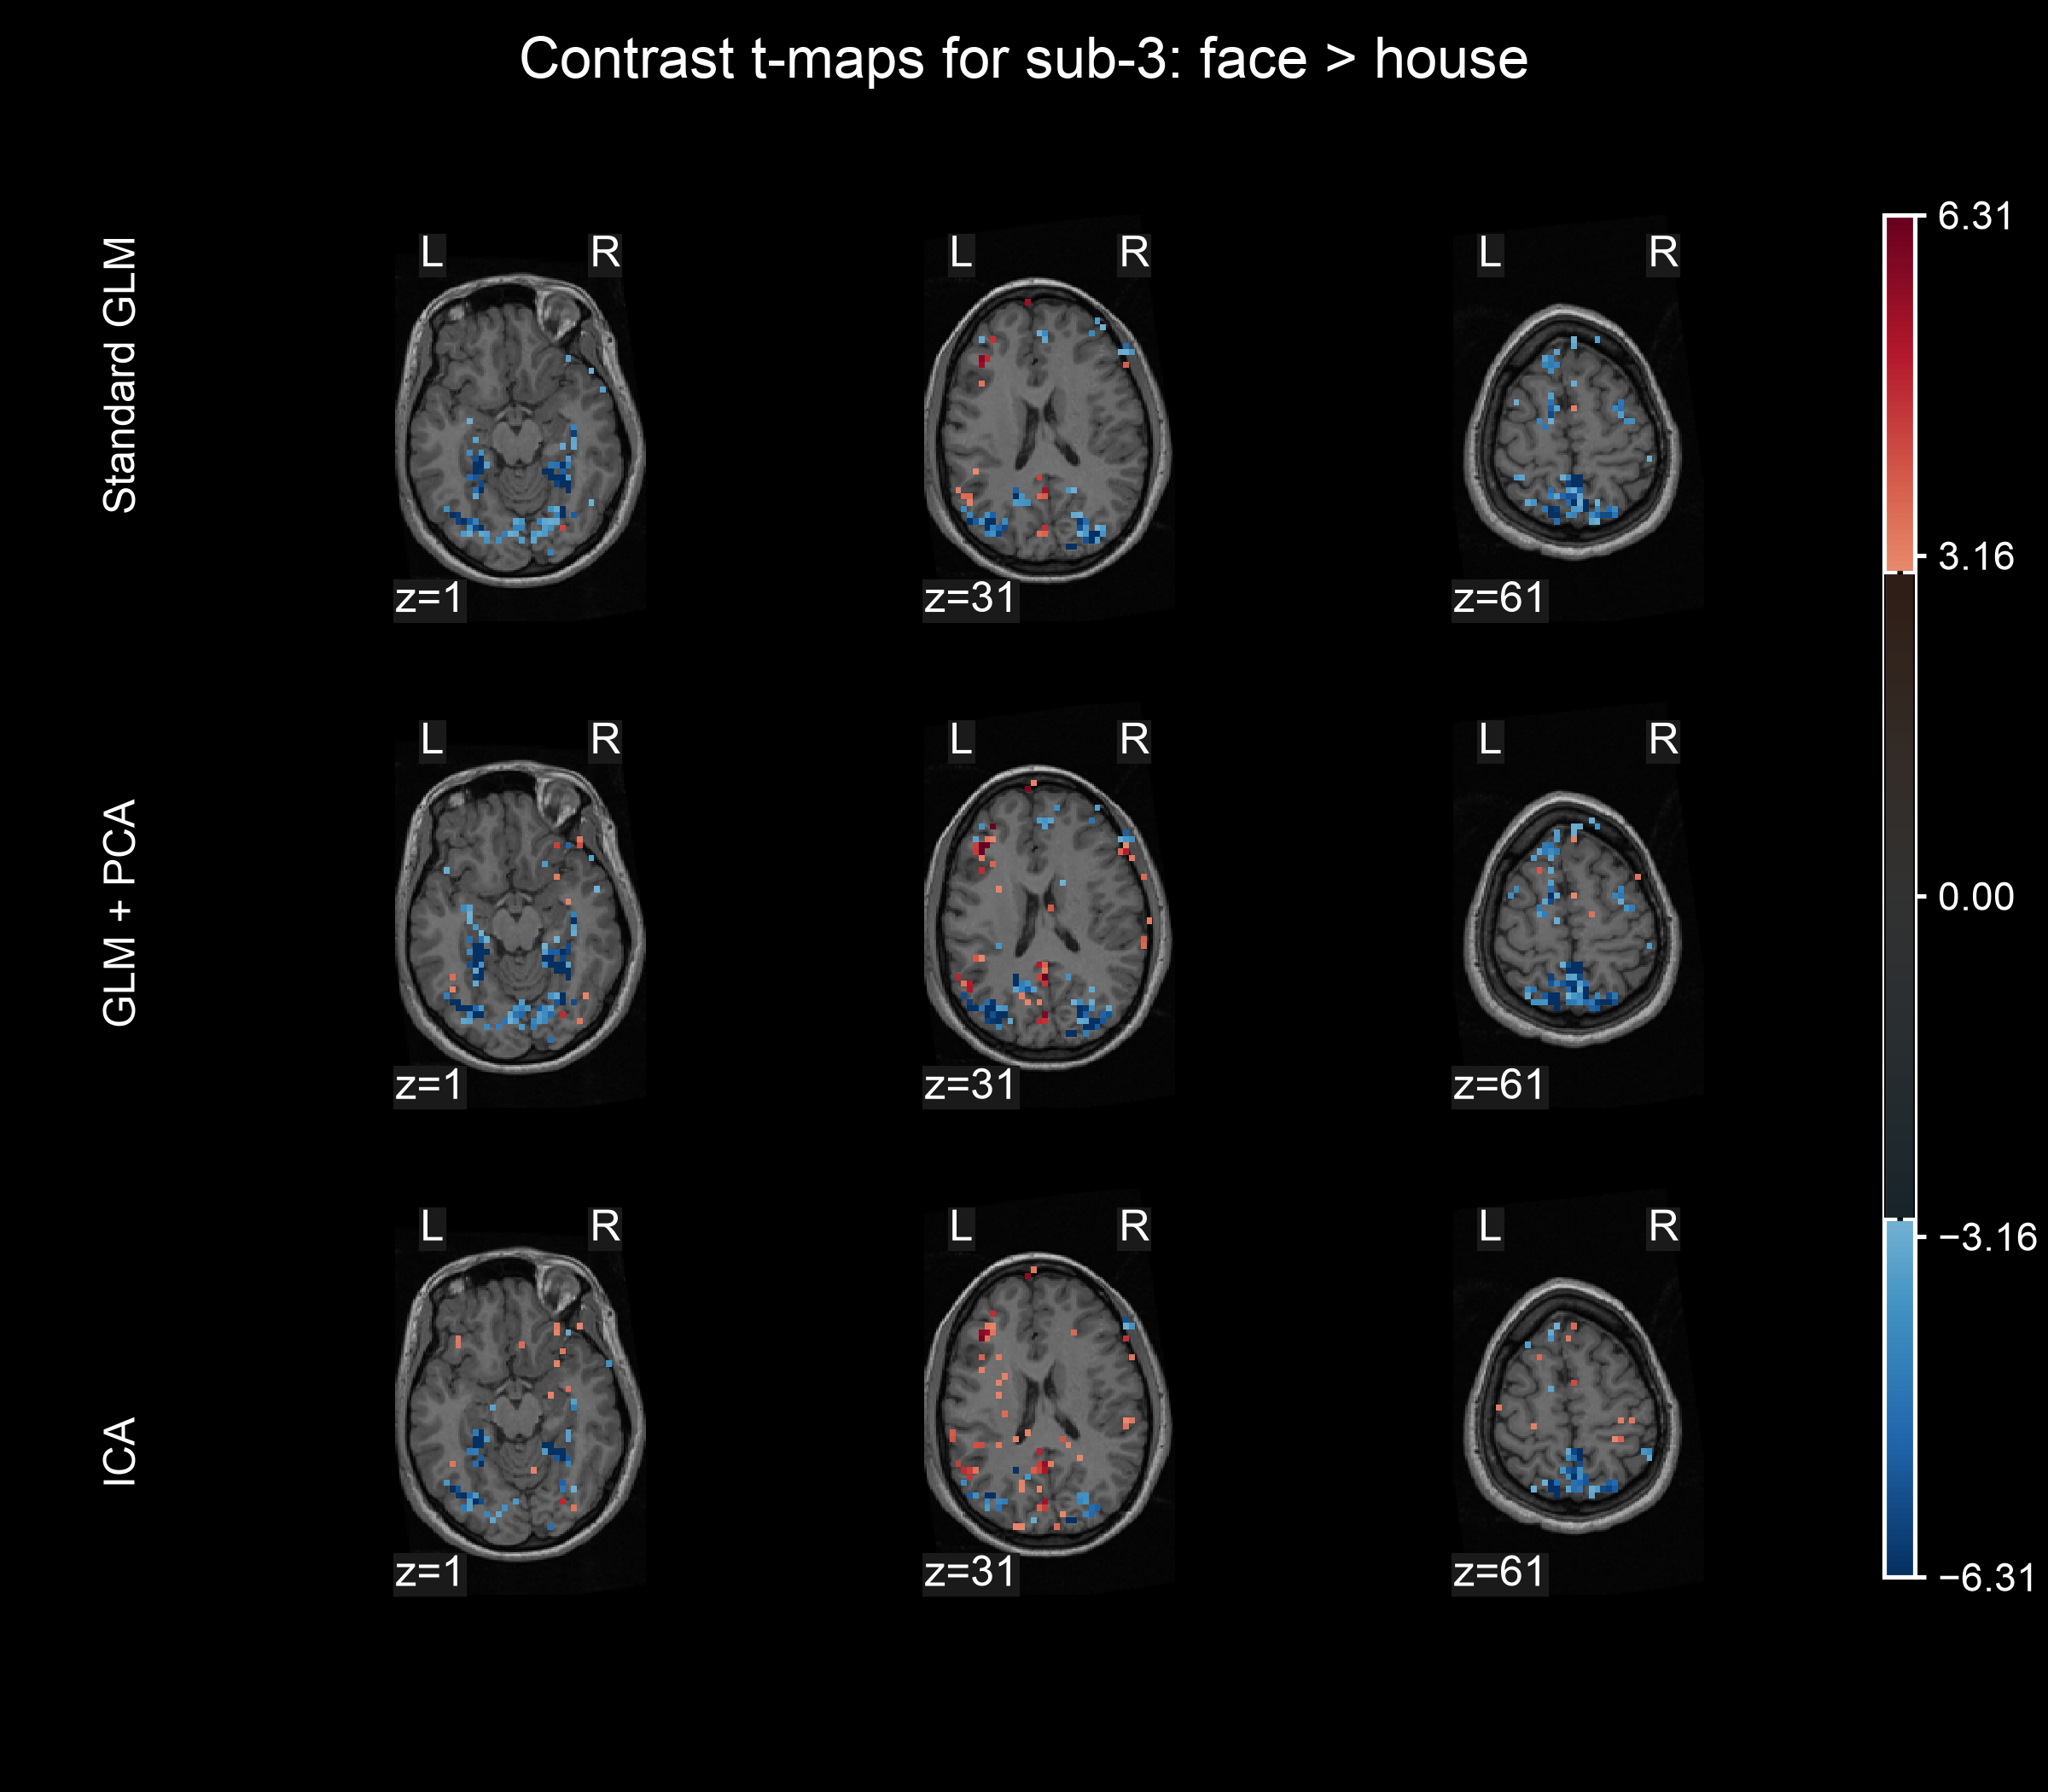
\includegraphics[scale=0.5]{fig/sub-3_t_face_vs_house.png}
    \caption{Slices along the $z$ axis of the $\text{face}-\text{house}$ contrast $t$-maps for subject 3 obtained with the standard GLM, PCA-assisted GLM denoising, and ICA-based denoising, shown using a common symmetric color scale over the T1-weighted anatomical image. Values with $|t|<3$ are not displayed.}
    \label{fig:t-maps}
\end{figure}

\newpage
Positive $t$-values on the contrast maps indicate evidence in the direction of a stronger face response, whereas negative $t$-values indicate evidence in the direction of a stronger house response. Across the displayed slices, negative values appear more spatially common than positive values for the standard GLM and PCA-assisted GLM. An exception can be observed at $z=31$, where both positive and negative regions are present, particularly for PCA-assisted GLM denoising. For ICA-based denoising, the same slice contains a visibly larger extent of positive regions. Overall, a substantial portion of the displayed standardized contrast effects is therefore directed towards a stronger response to houses than to faces.

The standard GLM and PCA-assisted GLM maps are again spatially similar. Across all three slices, many positive and negative regions occur in similar locations, with the dominant negative regions being particularly well preserved. At $z=1$, both methods show pronounced negative face-versus-house contrast values in similar regions, although PCA-assisted GLM denoising introduces some differences in the extent and magnitude of both positive and negative values. At $z=31$, both maps contain a mixture of positive and negative regions, with PCA generally showing a somewhat greater spatial extent. At $z=61$, both methods are dominated by negative regions and closely resemble one another.

Interestingly, the ICA contrast maps do not differ as substantially from the GLM-based methods at $z=1$ and $z=61$, where several of the dominant negative regions remain recognizable. The largest difference is observed at $z=31$, where ICA exhibits fewer spatial negative regions and a substantially greater extent of positive values. Moreover, some spatial correspondence is retained, although local patterns differ, particularly visible at $z=1$. Thus, although ICA preserves parts of the broader contrast pattern, its spatial distribution of standardized contrast effects departs more strongly from the two GLM-based methods. This observation is consistent with the poorer prediction accuracy and lower jackknife SNR previously obtained for ICA-based denoising.

\section{Runtime analysis}

\begin{figure}[!htbp]
    \centering
    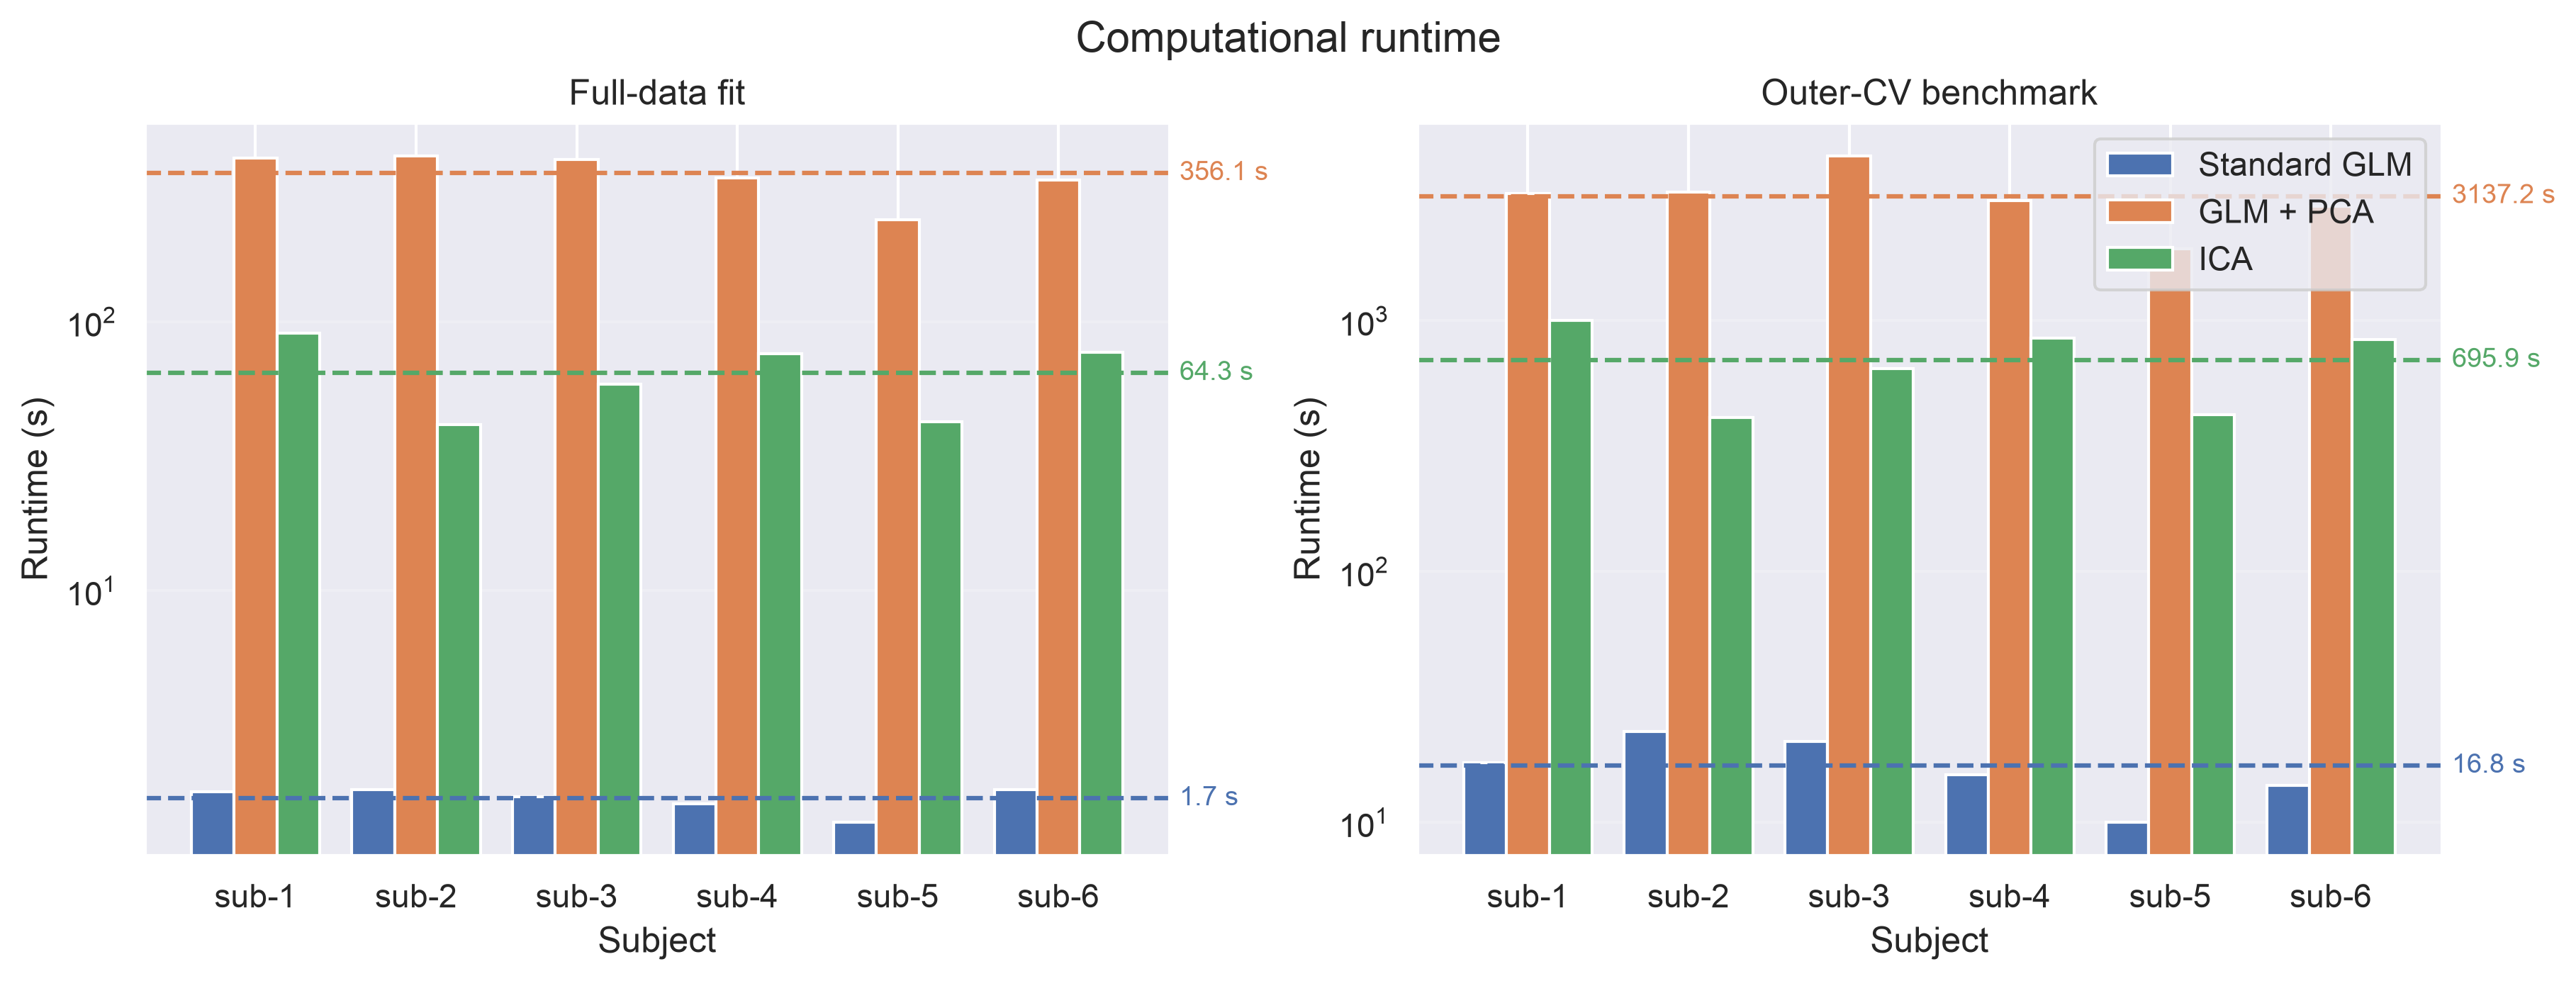
\includegraphics[width=\textwidth]{fig/runtime.png}
    \caption{Runtime of the analyzed methods for the full-data fit (left) and outer-CV benchmark (right) across subjects, shown on a logarithmic scale; dashed horizontal lines indicate mean runtime across subjects.}
    \label{fig:runtime}
\end{figure}

\newpage
Lastly, the computational runtime of the analyzed methods was compared. Figure~\ref{fig:runtime} presents two bar plots showing the runtime in seconds for each method and subject on a base-10 logarithmic scale. The left subplot presents the runtime of the full-data fit, whereas the right subplot presents the total runtime of the outer-CV benchmark. Horizontal dashed lines indicate the average runtime of each method across subjects.

The most computationally expensive method is PCA-assisted GLM denoising, with a mean runtime of $356.1$ seconds for the full-data fit and $3137.2$ seconds for the outer-CV benchmark. ICA-based denoising is the second most time-consuming method, with corresponding mean runtimes of $64.3$ and $695.9$ seconds. The fastest method by a substantial margin is the standard GLM, requiring on average only $1.7$ seconds for the full-data fit and $16.8$ seconds for the outer-CV benchmark.

Runtime is relatively consistent across subjects within each method, although some variability is present. Subject 5 generally requires less computation, particularly during the outer-CV benchmark. This is expected because subject 5 contains only 11 runs rather than the 12 available for the remaining subjects, as described in Section~\ref{section:caveats}.

The substantially lower computational cost of the standard GLM follows from its simpler estimation procedure. Unlike PCA-assisted GLM denoising, it does not require the construction and cross-validation of additional PCA-derived nuisance regressors. The inner cross-validation procedure used to select the number of PCA noise regressors substantially increases the computational cost of PCA-assisted GLM denoising. ICA-based denoising additionally requires model-order selection, iterative ICA estimation, permutation-based component classification, and subsequent reconstruction of the denoised data, resulting in a considerably longer runtime than the standard GLM.

The computational efficiency of the standard GLM is particularly notable in view of its prediction accuracy. As shown in Section~\ref{section:prediction-results}, PCA-assisted GLM denoising generally improves outer-CV prediction accuracy only by a relatively small amount despite its substantially greater computational cost.

The poor prediction accuracy of ICA-based denoising is similarly accompanied by considerably greater computational cost. On average, ICA requires approximately $38$ times the runtime of the standard GLM for the full-data fit and approximately $41$ times the runtime for the outer-CV benchmark, while producing lower prediction accuracy for several subjects.

Overall, the standard GLM provides the most favorable trade-off between computational cost and prediction accuracy among the analyzed methods. PCA-assisted GLM denoising provides small improvements in prediction accuracy at a substantial computational cost, whereas the considered ICA-based denoising procedure is both computationally more expensive and, for several subjects, less accurate than the standard GLM.


\section{Remarks about results}
\label{section:results-remarks}

Considering outer cross-validated prediction accuracy as the primary evaluation criterion, PCA-assisted GLM denoising was the best-performing method in the analyzed dataset. It achieved the highest median prediction accuracy for all participants. However, the improvement relative to the standard GLM was small. In contrast to prediction accuracy, PCA-assisted GLM denoising did not consistently improve the stability of the task-related coefficient estimates. For several subjects, the jackknife SNR was lower than for the standard GLM, while for the remaining subjects the differences were smaller and varied across voxels. 

The PCA-assisted method was also the most computationally expensive method in the present implementation. The standard GLM therefore provided the most favorable trade-off between prediction accuracy, coefficient stability, and computational cost. Its prediction accuracy was only slightly below that of PCA-assisted GLM denoising, while its runtime was substantially lower.

ICA-based denoising produced the weakest overall results. Its prediction accuracy was lower than that of the standard GLM for subjects 1–4, whereas subjects 5 and 6 showed only small positive improvements. The same subject-dependent pattern was visible in the jackknife SNR analysis, where ICA-based estimates were generally less stable for the subjects with the largest deterioration in prediction accuracy. ICA was also considerably more computationally expensive than the standard GLM. Consequently, under the considered implementation and dataset, the additional complexity of ICA-based denoising was not accompanied by an improvement in task-response estimation.

The magnitude of the improvement obtained using PCA-assisted GLM denoising is smaller than that reported for GLMdenoise in \cite{glm-denoise}. Several methodological and experimental differences may explain this result. 

One possible factor is the strength of the standard GLM used in the present analysis. Whereas the original GLMdenoise implementation uses Ordinary Least Squares, the present thesis uses Feasible Generalized Least Squares with an estimated autoregressive temporal covariance structure. The standard GLM additionally contains DCT drift regressors. Consequently, part of the temporally structured variability may already be accounted for before PCA-derived nuisance regressors are introduced. This may reduce the additional benefit obtainable from the PCA regressors. 

A second important difference is the experimental design. The datasets considered in~\cite{glm-denoise} used event-related designs containing between 9 and 156 relatively short conditions. In contrast, the dataset considered in this thesis contains eight visual categories presented in 24-second blocks. Block designs generally produce sustained BOLD responses with relatively high detection sensitivity \cite{glm-denoise}. The repeated and temporally extended responses may therefore already be estimated relatively well by the standard GLM, leaving less room for additional nuisance regressors to improve prediction accuracy. This provides a plausible explanation for the consistently positive but small improvement obtained with PCA-assisted GLM denoising.

The absolute cross-validated $R^2$ values should also not be compared directly with those reported in \cite{glm-denoise}. Apart from the different experimental designs, the analyses differ in preprocessing, HRF estimation, drift modeling, acquisition characteristics, and the definition of the voxel set used for summarizing performance. In particular, the present implementation uses a fixed canonical HRF, whereas the original GLMdenoise procedure estimates a dataset-specific HRF. 

Several additional factors may account for the poorer performance of ICA-based denoising. The component-classification results showed a substantial concentration of task-related component scores around the threshold $c=0$, without a clear separation between task-related and nuisance components. Consequently, the classification is sensitive to relatively small changes in the task-related score. Components containing useful task-related information may therefore occasionally be removed, while nuisance-dominated components may be retained. Because ICA components are removed by reconstruction and subtraction before the subsequent FGLS analysis, faulty classification can appear and influence the signal available for estimation.

\newpage
The estimated ICA model orders provide another possible explanation. For several runs, the selected number of components is large relative to the 121 available time points. Consequently, only limited dimensionality reduction is performed in these cases. Estimating a large number of independent components from a relatively short time series may produce components that are less stable and more difficult to classify reliably. Since the model-order selection and FastICA procedures used here are not identical to those implemented in \cite{glm-denoise}, this represents an additional difference from the ICA-based benchmark in \cite{glm-denoise}.

Finally, the preprocessing of the analyzed data differs from that used in \cite{glm-denoise}. In particular, explicit motion correction was not applied in the present analysis, whereas the datasets used by the authors of \cite{glm-denoise} were preprocessed with motion correction. Subject motion changes the spatial correspondence of voxel measurements over time and may therefore affect both regression-based estimation and the ICA decomposition. Its absence may have contributed to the observed results, especially for ICA, whose estimated spatial components can be strongly influenced by motion-related variability. This limitation should therefore be considered when interpreting comparisons with previously published results.

Overall, the results do not indicate that PCA- or ICA-based denoising is generally ineffective. Rather, they show that the benefit of additional component-based denoising depends strongly on the experimental design, preprocessing procedure, baseline statistical model, and component-selection strategy. For the present dataset and implementation, PCA-assisted GLM denoising provided a small improvement in predictive accuracy at substantial computational cost, while the standard GLM provided a competitive and considerably simpler baseline. ICA-based denoising was more sensitive to methodological choices and produced less reliable results for several subjects.

\chapter{Conclusions}
\label{chapter:conclusions}

Denoising of fMRI data is an important part of obtaining reliable estimates of task-related brain responses. The neuroimaging literature emphasizes both the importance of reducing unwanted variability and the need for careful selection of denoising procedures, since overly aggressive denoising may also remove the part, which is of interest.

This thesis focused on statistical methods for fMRI data denoising. The analyzed dataset and its experimental structure were described together with the necessary neuroimaging nomenclature. Three denoising approaches were then presented and compared: the standard GLM denoising, PCA-assisted GLM denoising, and ICA-based denoising. The mathematical foundations, necessary derivations, and computational procedures for the considered methods were introduced.

A common regression-based framework was developed by extending the ordinary least-squares model with an estimated autoregressive temporal covariance structure. This covariance structure was used to prewhiten the data and the design matrix, resulting in a Feasible Generalized Least Squares procedure. FGLS subsequently formed the common basis for comparison of the considered methods.

The General Linear Model was introduced together with the construction of a design matrix consisting of task-related and nuisance regressors. The task-related regressors were constructed by convolving the experimental stimulus functions with a canonical haemodynamic response function, which models the expected BOLD response to the presented stimuli. The nuisance part of the standard GLM consisted primarily of an intercept and DCT-based drift regressors representing low-frequency signal variation. The PCA-assisted GLM additionally introduced data-derived nuisance regressors. A noise pool was first constructed from voxels with poor inner leave-one-run-out cross-validated task prediction, after which Principal Component Analysis was performed on the corresponding time series. An second inner leave-one-run-out cross-validation procedure selected the number of principal components included as additional nuisance regressors.

The GLM-based approaches were complemented by an ICA-based denoising method. The probabilistic ICA framework was used to motivate dimensionality reduction and the estimation of the latent source-space dimension. Before model-order estimation, the data were temporally prewhitened with respect to the estimated noise covariance. Probabilistic PCA and approximate Bayesian model evidence were then used to select the model order and project the data onto the corresponding lower-dimensional subspace. After a separate ICA whitening step, the independent components were estimated using the symmetric FastICA algorithm. A permutation-based procedure was subsequently used to classify the estimated components as task-related or nuisance. The contribution of the components classified as nuisance was reconstructed and subtracted from the original data. Finally, the ICA-denoised data were analyzed using the same FGLS framework as the remaining methods.

Outer cross-validation using a leave-one-run-out procedure was performed separately for each of the analyzed methods. In each fold, one run was left out as the test set, while the remaining runs were used for model fitting. The fitted task-related coefficients were then used to predict the left-out run. Repeating this procedure across all runs provided predictions for the complete dataset and allowed prediction accuracy and coefficient stability to be evaluated under a common framework. Additional full-data analyses, including spatial maps and runtime measurements, complemented the cross-validation-based evaluation.

The prediction-accuracy results indicated a small but consistent improvement after introducing PCA-derived nuisance regressors. PCA-assisted GLM denoising achieved the highest median outer-CV $R^2$ for every analyzed subject. The mean of the median prediction accuracies was $1.62\%$ for PCA-assisted GLM denoising and $1.48\%$ for the standard GLM, corresponding to an average difference of approximately $0.14$ percentage points. The improvement was therefore positive, but small. Moreover, this improvement did not translate into consistently greater stability of the task-related coefficient estimates. For several subjects, PCA-assisted GLM denoising produced a jackknife signal-to-noise ratio values, which were lower than, or similar to the standard GLM. The beta and contrast maps obtained with the two GLM-based methods were also spatially similar, indicating that the additional PCA regressors generally modified rather than fundamentally changed the estimated task-response patterns.

The standard GLM performed only marginally worse than PCA-assisted GLM denoising in terms of prediction accuracy while being substantially less computationally expensive. The average full-data fitting time was approximately $1.7$ seconds for the standard GLM, compared with $356.1$ seconds for PCA-assisted GLM denoising. For the complete outer cross-validation benchmark, the corresponding average runtimes were $16.8$ and $3137.2$ seconds. Therefore, for the considered dataset and implementation, the standard GLM provided a favorable trade-off between prediction accuracy, stability, model complexity, and computational cost.

ICA-based denoising generally produced the weakest results among the three considered approaches. Its mean median outer-CV $R^2$ was $0.76\%$, compared with $1.48\%$ for the standard GLM. Prediction accuracy deteriorated particularly for subjects 1--4, whereas only small improvements relative to the standard GLM were observed for subjects 5 and 6. The ICA-derived estimates also showed lower stability for several subjects, and their spatial beta and contrast maps departed more strongly from the two GLM-based methods. The component analysis and final remarks about results suggested several possible explanations for these results. The selected ICA model orders varied substantially between runs, and many component task-association scores were located close to the classification threshold. Consequently, the component-classification procedure may not have provided sufficiently robust separation between task-related and nuisance components. Additional factors include differences in the experimental design and preprocessing of the analyzed dataset, including the absence of explicit motion correction.

The computational cost of the component-based methods further limits the practical benefit observed in this analysis. PCA-assisted GLM denoising was the most computationally expensive method, while ICA-based denoising required an average of $64.3$ seconds for the full-data fit and $695.9$ seconds for the complete outer-CV benchmark. Thus, the increased computational complexity of the component-based approaches was not accompanied by a proportional increase in predictive performance. PCA-assisted GLM denoising produced only a modest improvement over the standard GLM, whereas ICA-based denoising generally reduced prediction accuracy.

Nonetheless, the analysis illustrates several important properties of statistical fMRI denoising. In particular, increasing model complexity does not necessarily lead to proportionally better task-response estimates. The effectiveness of a denoising procedure depends on the experimental design, noise structure, preprocessing, selection of nuisance components, and statistical model used for subsequent estimation. For the dataset considered in this thesis, PCA-assisted GLM denoising achieved the highest predictive performance, whereas the substantially simpler standard GLM remained highly competitive. ICA-based denoising proved more sensitive to methodological choices and produced strongly subject-dependent results.

% styl bibliografii, tutaj unsrt
\bibliographystyle{plain}
% w nawiasie klamrowym wpisujemy nazwę pliku z bibliografią w formacie .bib
\bibliography{bibliografia} 
\end{document} 